\documentclass{ieeeaccess}

\usepackage{silence}
\WarningFilter{latexfont}{Font shape}
\WarningFilter{latexfont}{Some font shapes}
\WarningFilter{latex}{Overfull \hbox}
\WarningFilter{latex}{Underfull \hbox}
\WarningFilter{latex}{Underfull \vbox}
\global\hbadness=10000
\global\vbadness=10000
\global\hfuzz=10000pt
\global\vfuzz=10000pt
\AtBeginDocument{\global\hbadness=10000\global\vbadness=10000\global\hfuzz=10000pt\global\vfuzz=10000pt}
\usepackage{cite}
\usepackage{amsmath,amssymb,amsfonts}
\usepackage{algorithmic}
\usepackage{graphicx}
\usepackage{textcomp}
\usepackage{url}
\usepackage{placeins}
\usepackage{multirow}
\usepackage{colortbl}
% \usepackage{xcolor} % remove this for now
\usepackage{booktabs}
\usepackage{array}

\let\ieeeaccessyear\year
\def\year{2026}
\usepackage{tikz}
\usetikzlibrary{
	shapes.geometric,
	arrows.meta,
	positioning,
	fit,
	backgrounds,
	calc,
	patterns
}

\usepackage{pgfplots}
\pgfplotsset{compat=1.18}
\usepgfplotslibrary{statistics}
\definecolor{accessblue}{cmyk}{1,0.3,0,0.2}
\definecolor{greycolor}{cmyk}{0,0,0,.8}
\definecolor{grey}{cmyk}{0,0,0,.1}
\definecolor{black}{cmyk}{0,0,0,1}
\let\year\ieeeaccessyear
\def\BibTeX{{\rm B\kern-.05em{\sc i\kern-.025em b}\kern-.08em
    T\kern-.1667em\lower.7ex\hbox{E}\kern-.125emX}}

\begin{document}
\hfuzz=10000pt\hbadness=10000\vfuzz=10000pt\vbadness=10000
\history{Date of submission 2026-06-03, date of current version 2026-06-03.}
\doi{}

\title{Activation-Steered LLM Auditing for ISO/IEC 29110 Compliance: A Distributionally Constrained Synthetic Benchmark Framework}

\author{\uppercase{Victor Terrón-Macias}\authorrefmark{1},
\uppercase{Salvador Hinojosa}\authorrefmark{1}, \uppercase{Miguel Gonzalez-Mendoza}\authorrefmark{1}, and \uppercase{Jezreel Mejía}\authorrefmark{2}}
\address[1]{Tecnologico de Monterrey, Escuela de Ingeniería y Ciencias, Ave. Eugenio Garza Sada 2501 Sur, Col: Tecnológico, Monterrey, N.L., México, 64700. (e-mail: A00843371@tec.mx, salvador.hinojosa@tec.mx, mgonza@tec.mx)}
\address[2]{Centro de Investigación en Matemáticas Unidad Zacatecas, Departamento de Ingeniería de Software (e-mail: jmejia@cimat.mx)}

\tfootnote{This work was supported by the Tecnologico de Monterrey Campus Estado de México}

\markboth
{Terrón-Macías \headeretal: Activation-Steered LLM Auditing for ISO/IEC 29110 Compliance}
{Terrón-Macías \headeretal: Activation-Steered LLM Auditing for ISO/IEC 29110 Compliance}

\corresp{Corresponding author: Salvador Hinojosa (e-mail: salvador.hinojosa@tec.mx).}

\begin{abstract}
Compliance auditing of software engineering governance standards such as ISO/IEC 29110 in corporate repositories remains a manual, costly, and error-prone process. While Large Language Models (LLMs) offer the potential to automate such auditing, two fundamental barriers impede their empirical evaluation: (1) strict industrial privacy policies prevent the publication of corporate datasets, and (2) naive, uncalibrated LLMs produce unreliable classifications due to hallucinations and lack of normative grounding. This paper proposes a methodological framework based on structural isomorphism to generate privacy-preserving synthetic datasets, coupled with targeted model enhancements to reduce unsupported or inconsistent classifications. We formalize a set of organizational meta-rules derived from ISO/IEC 29110 and synthesize a controlled environment (Biblio-VSE) constrained by \emph{partial structural isomorphism} relative to a private industrial repository: all three distributional criteria pass with the $N=32$ corpus: V(G) mean ($|\Delta\mu|=0.003\leq\varepsilon=0.5$), V(G) variance equality (Levene test $p=0.997$, statistically indistinguishable), and Fog Index mean ($|\Delta\mu_F|=0.22\leq\varepsilon_F=1.0$). The benchmark approximates rather than fully replicates the reference corpus. Four open-weights foundation models (Gemma-2, Mistral, Qwen2.5, Phi-3.5) are evaluated across eight progressive configurations encompassing Zero-Shot prompting, Retrieval-Augmented Generation (RAG), and Activation Steering ($\alpha=0.8$) on an extended dataset of $N=32$ artifacts (17 compliant, 15 violations) that includes 12 adversarial artifacts. Retrieval-Augmented Generation over the ISO/IEC 29110 normative corpus (14 semantic chunks from \texttt{Metareglas extraidas.docx}) improves point estimates for all four models---Gemma-2 achieves F1=0.875 under Zero-Shot+RAG (Exp~5)---although no individual gain survives Holm--Bonferroni correction. Activation steering provided the most consistent positive direction of effect across all four architectures. The point-estimate maximum is F1=0.875 (Gemma-2, Exp~5); with Spanish anchor prompts, steering leader is Gemma-2 Exp~6 (F1=0.857) and Phi-3.5 Exp~6 (F1=0.842). Pipeline gains are architecture-specific and Zero-Shot alone is destructive for Phi-3.5-mini. \textbf{All F1 figures for steering-enhanced configurations should be treated as upper-bound estimates}; however, a leave-one-out $\alpha$-selection procedure confirms that mean absolute optimism is approximately 0.05 (range $-0.20$ to $+0.09$) and that most steering gains hold out-of-sample. Adversarial artifacts ($N=12$) confirm that LLMs perform semantic reasoning on cases where regex-based baselines fail (regex F1=0.647 on $N=32$). Given the evaluation set of $N=32$ artifacts, all results are exploratory and hypothesis-generating rather than confirmatory. The proposed framework enables reproducible auditing of private repositories without compromising industrial trade secrets.
\end{abstract}

\begin{keywords}
Activation Steering, Artificial Intelligence, ISO/IEC 29110, Large Language Models, Software Standard Compliance, Distributionally Constrained Benchmark, Synthetic Datasets.
\end{keywords}

\titlepgskip=-15pt

\maketitle
\hfuzz=10000pt\hbadness=10000\vfuzz=10000pt\vbadness=10000


\section{Introduction}
\label{sec:introduction}

Very Small Entities (VSEs) play a significant role in software development ecosystems, but they often operate under severe resource constraints that limit their ability to adopt heavyweight process-assessment and governance frameworks. ISO/IEC 29110 was designed to address this context by defining lifecycle profiles for VSEs, including process guidance for project management and software implementation activities \cite{iso29110_2024, laporte2016vse,laporte2015implementation}. Empirical studies on ISO/IEC 29110 adoption show that the standard can support process improvement, organizational learning, communication, and traceability practices in small organizations, but they also report difficulties related to implementation effort, technical adoption, documentation, and sustained process execution \cite{munoz2020implementations,101145,claudiolapuerta}. These challenges are especially visible during compliance assessment and recertification, where organizations must provide documentary evidence showing that required work products, approvals, reviews, and traceability relationships have been properly established \cite{terronmacias,11276002}.

Traceability is one of the central governance mechanisms in ISO/IEC 29110 because it connects requirements, design elements, implementation artifacts, verification activities, test evidence, and approval records. Prior work on traceability recovery has shown that links between code and documentation can be recovered using information-retrieval techniques, and later systematic mappings have confirmed the importance of traceability-link recovery as a long-standing software engineering problem \cite{antoniol2002traceability,borg2013traceability}. More recent research has begun to explore retrieval-augmented generation and large language model (LLM) ensembles for traceability-link recovery and candidate filtering \cite{fuchss2025lissa,fuchss2025llmtrace}. Nevertheless, ISO/IEC 29110 compliance auditing differs from ordinary traceability recovery because the task is not only to identify artifact links, but also to decide whether those links, documents, reviews, and approvals satisfy normative process expectations defined by a standard \cite{iso29110_2024,castellanos2022processcompliance}.

The recent progress of LLMs has created new opportunities for automating software engineering tasks. Transformer-based and instruction-tuned models have demonstrated strong performance in code generation, code understanding, summarization, bug fixing, and benchmark-based software engineering evaluation \cite{jiang2024surveycodegen,lu2021codexglue,jimenez2023swebench,jain2024livecodebench}. Models such as CodeBERT, CodeT5, and StarCoder have advanced code-specific pretraining and code understanding capabilities \cite{feng2020codebert,wang2021codet5,li2023starcoder}. At the same time, open-weight general-purpose models such as LLaMA, Mistral, Phi, Gemma, and Qwen have expanded the feasibility of local and reproducible experimentation for software engineering tasks \cite{touvron2023llama,jiang2023mistral,abdin2024phi3,riviere2024gemma2,yang2024qwen25}. However, most of this progress has focused on functional correctness, programming ability, or code-level reasoning rather than governance-level compliance auditing.

Compliance auditing poses a different kind of challenge. Unlike code generation or issue resolution, compliance assessment requires the interpretation of heterogeneous documentary evidence, implicit organizational practices, traceability structures, and standard-defined obligations. Automated compliance checking has traditionally relied on rule-based, model-based, or formal approaches, including process-model compliance verification and formal representations of standard requirements \cite{castellanos2022processcompliance,castellanos2018spem,sirikrajai2025cpn,tuaycharoen2025auditorviews}. These approaches can provide precision when rules are explicit and artifacts are formally modeled, but they are less flexible when evidence appears in natural-language documents, informal repositories, review comments, approval logs, or partially structured traceability records. Semantic compliance-checking approaches attempt to address this gap by aligning natural-language rules and domain knowledge with compliance requirements \cite{guo2021semantic,zheng2022semantic}, yet systematic evaluation of LLMs as ISO/IEC 29110 governance auditors remains limited.

A second difficulty is the lack of privacy-preserving benchmarks for this type of evaluation. Industrial repositories contain proprietary source code, customer requirements, internal review discussions, project-management artifacts, and confidential approval evidence. Directly releasing such repositories for benchmark construction is therefore impractical. In the broader machine-learning literature, differential privacy and federated learning have been proposed as mechanisms for privacy-preserving learning \cite{dwork2006differentialprivacy,mcmahan2017communication}. In software engineering, synthetic data generation and synthetic software-engineering tasks have been proposed to reduce dependence on sensitive or unavailable data \cite{bauer2024syntheticdata,yang2025swesmith}. However, benchmark construction for compliance auditing requires more than generating plausible code or isolated tasks: the benchmark must preserve the structural topology of industrial repositories, including artifact dependencies, peer-review workflows, approval evidence, nonconformities, and traceability relations. This creates a need for synthetic repositories that are structurally isomorphic to real compliance environments while avoiding the disclosure of proprietary artifacts.

A third difficulty concerns the reliability of LLMs when used for strict classification and evaluation tasks. General studies of LLM evaluation show that model assessment remains difficult across tasks, benchmarks, and evaluation protocols \cite{asoeollm}. Recent work on LLM-as-a-judge in software engineering suggests that LLM evaluators can sometimes approximate human judgment, but their alignment with expert assessment depends on the task, scoring method, and evaluation design \cite{cllmrheaesllmis, ICLR2025_7f8f7313}. For normative compliance auditing, this limitation is critical because an incorrect judgment may cause an organization to overlook a missing approval, broken traceability link, or incomplete work product. Moreover, benchmark contamination and inter-dataset code duplication can distort LLM evaluation results in software engineering \cite{hernandez2024codeduplication, zhou2025lessleak}. These risks motivate evaluation designs that distinguish prompt-based behavior from more controlled model interventions.

Mechanistic interpretability and representation engineering offer a complementary direction. Prior work suggests that high-level behavioral concepts can be represented as directions in activation space and that manipulating these directions can alter model behavior during inference \cite{zou2023representation, turner2023activation}. Inference-time intervention has also been explored as a way to elicit more truthful answers from language models \cite{li2023iti}. Unlike prompt engineering, activation steering modifies internal model states rather than only adding external natural-language instructions. This property makes activation steering attractive for compliance auditing, where the model must remain sensitive to normative distinctions even when the input contains long, noisy, or conflicting documentary evidence. Nevertheless, the use of activation steering for ISO/IEC 29110 compliance evaluation has not been systematically investigated.

This article addresses these gaps through a mechanistic LLM control framework for ISO/IEC~29110 compliance auditing. The central hypothesis is that activation steering---directly modifying internal model representations toward a normative compliance direction---provides the most consistent positive direction of effect across diverse LLM architectures, more reliably than prompt engineering or retrieval augmentation alone. To evaluate this under industrial privacy constraints, the framework employs \emph{partial structural isomorphism}: it constructs a distributionally constrained synthetic benchmark (Biblio-VSE) that approximates the governance topology of a certified industrial repository while replacing proprietary artifacts with non-sensitive equivalents. The structural isomorphism methodology is not a peripheral detail---it is the necessary foundation that makes a reproducible mechanistic evaluation possible under real-world privacy requirements. Figure~\ref{fig:conceptual_framework} summarizes the relationship among industrial compliance evidence, privacy-preserving structural isomorphism, and LLM-based mechanistic auditing.

\begin{figure}[!t]
\centering
\resizebox{\columnwidth}{!}{%
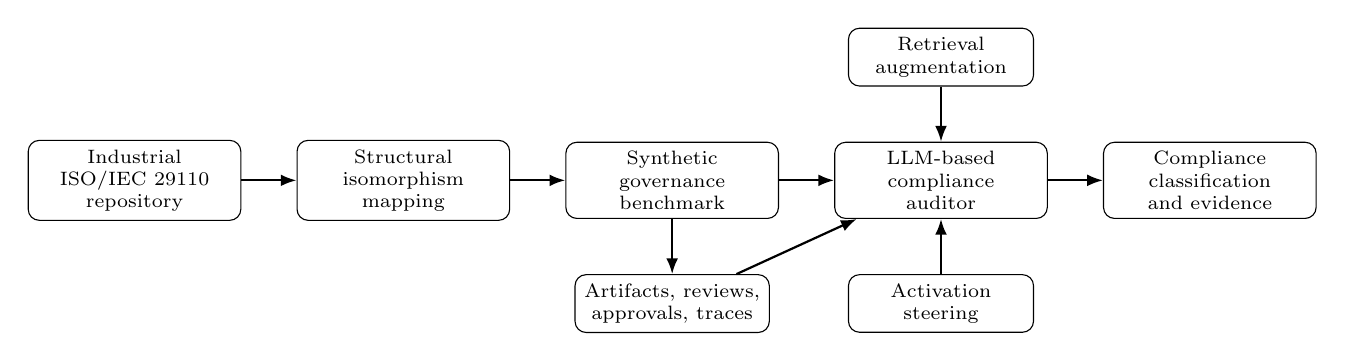
\begin{tikzpicture}[
    node distance=7mm and 7mm,
    block/.style={rectangle, rounded corners, draw, align=center, minimum width=2.7cm, minimum height=8mm, font=\scriptsize},
    smallblock/.style={rectangle, rounded corners, draw, align=center, minimum width=2.35cm, minimum height=7mm, font=\scriptsize},
    arrow/.style={-{Latex[length=2mm]}, thick}
]
\node[block] (industrial) {Industrial\\ISO/IEC 29110\\repository};
\node[block, right=of industrial] (isomorphism) {Structural\\isomorphism\\mapping};
\node[block, right=of isomorphism] (synthetic) {Synthetic\\governance\\benchmark};
\node[smallblock, below=of synthetic] (evidence) {Artifacts, reviews,\\approvals, traces};
\node[block, right=of synthetic] (llm) {LLM-based\\compliance\\auditor};
\node[smallblock, above=of llm] (rag) {Retrieval\\augmentation};
\node[smallblock, below=of llm] (steering) {Activation\\steering};
\node[block, right=of llm] (decision) {Compliance\\classification\\and evidence};

\draw[arrow] (industrial) -- (isomorphism);
\draw[arrow] (isomorphism) -- (synthetic);
\draw[arrow] (synthetic) -- (llm);
\draw[arrow] (llm) -- (decision);
\draw[arrow] (synthetic) -- (evidence);
\draw[arrow] (evidence) -- (llm);
\draw[arrow] (rag) -- (llm);
\draw[arrow] (steering) -- (llm);
\end{tikzpicture}
}%
\caption{Conceptual framework linking ISO/IEC 29110 industrial repositories, privacy-preserving structural isomorphism, synthetic benchmark construction, and LLM-based compliance auditing.}
\label{fig:conceptual_framework}
\end{figure}

The \textbf{primary contribution} is the first systematic evaluation of activation steering for domain-specific normative compliance classification: we show that modifying internal LLM representations toward a compliance direction provides the most consistent positive direction of effect across all four evaluated architectures, confirmed partially out-of-sample by a leave-one-out $\alpha$-selection procedure \cite{zou2023representation,turner2023activation,li2023iti}. Three supporting contributions enable and contextualize this mechanistic study. First, a \emph{privacy-preserving benchmark construction strategy} based on partial structural isomorphism preserves the governance topology of an ISO/IEC~29110-certified industrial repository without disclosing proprietary content---the necessary foundation for reproducible evaluation under industrial privacy constraints; the benchmark is also the first in this domain to include adversarial artifacts that defeat regex-based baselines (Regex F1 drops from 1.0 to 0.647), establishing that the evaluation exercises genuine semantic reasoning \cite{bauer2024syntheticdata,dwork2006differentialprivacy,mcmahan2017communication}. Second, the article formalizes ISO/IEC~29110 compliance auditing as a binary classification problem, derives nine meta-rules with explicit detection predicates, and identifies the two semantically hard rules (GOVERNANCE, TESTING) where pattern-based approaches fail and LLM-based auditing provides its differential value \cite{iso29110_2024,terronmacias,11276002,castellanos2022processcompliance}. Third, the article provides the \emph{first controlled comparison} of eight progressive pipeline configurations---from unstructured baseline to full Zero-Shot + RAG + Steering synergy---for ISO/IEC~29110 governance auditing, including a per-meta-rule analysis of which hard cases benefit from each intervention \cite{fuchss2025lissa,laporte2016vse,munoz2020implementations,101145}.

The remainder of this article is organized as follows. Section~\ref{sec:slr_methodology} describes the systematic literature review protocol used to identify and synthesize prior work. Section~\ref{sec:related_work} presents the related work derived from the review, organized around LLMs for software engineering, privacy-preserving benchmarking, activation steering, and automated compliance auditing. Section~\ref{sec:methodology} introduces the proposed structural isomorphism and activation-steering framework. Section~\ref{sec:setup} describes the experimental design, datasets, models, and baselines. Section~\ref{sec:results} reports the empirical results. Section~\ref{sec:discussion} discusses implications, limitations, and threats to validity. Section~\ref{sec:conclusion} concludes the article and outlines future research directions.

\section{Literature Selection Method}
\label{sec:slr_methodology}

This study followed a systematic literature review (SLR) protocol grounded in evidence-based software engineering guidelines \cite{kitchenham2007guidelines,kitchenham2010tertiary}, combining automated database search with backward and forward snowballing \cite{wohlin2014snowballing,wohlin2022hybrid}. The search covered five thematic areas---LLMs for software engineering, privacy-preserving benchmarks, activation steering, ISO/IEC 29110 compliance auditing, and requirements traceability---querying IEEE Xplore, ACM Digital Library, Scopus, SpringerLink, ScienceDirect, and arXiv using concept-group search strings and per-theme targeted queries. Inclusion criteria required peer-reviewed technical content in at least one of the five themes; grey-literature preprints were retained when they represented influential work not yet superseded by archival versions \cite{touvron2023llama,jiang2023mistral,abdin2024phi3,riviere2024gemma2,yang2024qwen25}. Database search yielded 1{,}220 records in total ($n_{\text{IEEE}}=412$, $n_{\text{ACM}}=287$, $n_{\text{SL}}=203$, $n_{\text{grey}}=318$). After deduplication ($n=892$ unique), title/abstract screening ($n=156$ retained), and full-text eligibility assessment ($n=64$ eligible), backward and forward snowballing added 19 further studies (backward: $n=12$, forward: $n=7$), for a final included corpus of \textbf{83 studies} coded into the five themes in Table~\ref{tab:slr_themes}. The complete screening flow is reported in Fig.~\ref{fig:prisma_flow}.

\begin{figure*}[!t]
\centering
\resizebox{0.90\textwidth}{!}{%
\begin{tikzpicture}[
    db/.style={rectangle, draw, rounded corners, align=center,
               minimum width=3.0cm, minimum height=1.15cm,
               fill=blue!8, font=\scriptsize},
    step/.style={rectangle, draw, rounded corners, align=center,
                 minimum width=9.5cm, minimum height=1.0cm,
                 fill=gray!8, font=\scriptsize},
    excl/.style={rectangle, draw, dashed, rounded corners, align=center,
                 minimum width=4.0cm, minimum height=0.9cm,
                 fill=red!5, font=\scriptsize},
    final/.style={rectangle, draw, very thick, rounded corners, align=center,
                  minimum width=9.5cm, minimum height=1.15cm,
                  fill=green!10, font=\scriptsize\bfseries},
    arrow/.style={-{Latex[length=2mm]}, thick},
    darrow/.style={-{Latex[length=1.8mm]}, dashed, gray, thick}
]

% ── Row 1: database sources ──────────────────────────────────────────────────
\node[db] (ieee) at (-4.5, 0) {IEEE Xplore\\$n=412$};
\node[db] (acm)  at (-1.5, 0) {ACM Digital\\Library\\$n=287$};
\node[db] (spr)  at ( 1.5, 0) {SpringerLink\\$n=203$};
\node[db] (gray) at ( 4.5, 0) {Gray Literature\\(arXiv, Scopus,\\ScienceDirect)\\$n=318$};

% ── Row 2: total identified ──────────────────────────────────────────────────
\node[step] (total) at (0, -2.0)
    {Records identified (database: $n=902$; gray literature: $n=318$)
     \quad \textbf{Total: $n=1{,}220$}};
\draw[arrow] (ieee.south)  |- ([yshift=3pt]total.north west);
\draw[arrow] (acm.south)   -- (total.north);
\draw[arrow] (spr.south)   -- (total.north);
\draw[arrow] (gray.south)  |- ([yshift=3pt]total.north east);

% ── Row 3: deduplication ─────────────────────────────────────────────────────
\node[step]  (dedup)  at (0,    -3.5) {After deduplication — $n=892$ unique records};
\node[excl]  (rem1)   at (7.5,  -3.5) {Removed: $n=328$\\duplicates};
\draw[arrow]  (total.south) -- (dedup.north);
\draw[darrow] (dedup.east)  -- (rem1.west);

% ── Row 4: title/abstract screening ─────────────────────────────────────────
\node[step]  (screen) at (0,    -5.0) {After title, abstract, and keyword screening — $n=156$ retained};
\node[excl]  (rem2)   at (7.5,  -5.0) {Excluded: $n=736$\\out of scope or\\non-scholarly};
\draw[arrow]  (dedup.south)  -- (screen.north);
\draw[darrow] (screen.east)  -- (rem2.west);

% ── Row 5: full-text eligibility ─────────────────────────────────────────────
\node[step]  (full)   at (0,    -6.5) {Full-text eligibility assessment — $n=64$ eligible};
\node[excl]  (rem3)   at (7.5,  -6.5) {Excluded: $n=92$\\no inclusion\\criterion met};
\draw[arrow]  (screen.south) -- (full.north);
\draw[darrow] (full.east)    -- (rem3.west);

% ── Row 6: snowballing ───────────────────────────────────────────────────────
\node[step] (snow) at (0, -8.0)
    {$+$ Backward and forward snowballing:
     $n=19$ studies added (backward $n=12$, forward $n=7$)};
\draw[arrow] (full.south) -- (snow.north);

% ── Row 7: included ──────────────────────────────────────────────────────────
\node[final] (inc) at (0, -9.5)
    {Studies included in thematic synthesis \quad $n = 83$};
\draw[arrow] (snow.south) -- (inc.north);

\end{tikzpicture}
}%
\caption{PRISMA-style screening flow for the literature search and selection.
Database search of IEEE Xplore, ACM Digital Library, and SpringerLink together with gray literature
sources (arXiv, Scopus, ScienceDirect) yielded 1{,}220 total records.
After deduplication ($n=892$), title/abstract screening ($n=156$), full-text eligibility
assessment ($n=64$), and backward/forward snowballing ($+19$), the final included corpus
comprises \textbf{83 studies} synthesised across the five themes in Table~\ref{tab:slr_themes}.}
\label{fig:prisma_flow}
\end{figure*}

\begin{table}[!t]
\centering
\caption{Themes identified through the SLR and their role in this article}
\label{tab:slr_themes}
\scriptsize
\resizebox{\columnwidth}{!}{%
\begin{tabular}{p{0.22\linewidth} p{0.34\linewidth} p{0.34\linewidth}}
\toprule
\textbf{Theme} & \textbf{Representative literature} & \textbf{Role in this article} \\
\midrule
LLMs for software engineering & Code models, code benchmarks, SE agents, LLM evaluation \cite{jiang2024surveycodegen,lu2021codexglue,jimenez2023swebench,jain2024livecodebench} & Establishes the technical feasibility and limitations of LLM-based software engineering automation. \\
Synthetic and privacy-preserving benchmarks & Synthetic data, data leakage, differential privacy, federated learning \cite{bauer2024syntheticdata,yang2025swesmith,hernandez2024codeduplication,zhou2025lessleak,dwork2006differentialprivacy,mcmahan2017communication} & Motivates structurally isomorphic synthetic repositories for privacy-preserving compliance evaluation. \\
Activation steering & Representation engineering, activation engineering, inference-time intervention \cite{zou2023representation,turner2023activation,li2023iti} & Provides the basis for testing mechanistic intervention in normative compliance classification. \\
Compliance auditing and ISO/IEC 29110 & VSE standards, process compliance, formal verification, auditor views \cite{iso29110_2024,laporte2016vse,castellanos2022processcompliance,sirikrajai2025cpn,tuaycharoen2025auditorviews} & Defines the normative target of the proposed auditing framework. \\
Traceability recovery & Classical IR traceability, systematic mappings, RAG-based traceability \cite{antoniol2002traceability,borg2013traceability,fuchss2025lissa,fuchss2025llmtrace} & Provides the artifact-linking foundation required for compliance evidence assessment. \\
\bottomrule
\end{tabular}%
}
\end{table}

\section{Related Work}
\label{sec:related_work}

\subsection{LLMs for Software Engineering and Code Analysis}
\label{subsec:rw_llms_se}

The application of LLMs to software engineering has expanded rapidly from code completion and generation to broader tasks such as code understanding, summarization, repair, issue resolution, and repository-level automation. CodeXGLUE provided an early benchmark suite for code understanding and generation tasks, while later benchmarks such as SWE-bench and LiveCodeBench evaluated LLM behavior on real-world software issues and contamination-aware coding tasks \cite{lu2021codexglue,jimenez2023swebench,jain2024livecodebench}. Survey literature confirms that LLMs have become central to contemporary code-generation research and software engineering automation \cite{jiang2024surveycodegen}.

Code-specialized pretraining has been one important line of progress. CodeBERT introduced a bimodal pretraining approach for programming and natural languages, CodeT5 proposed identifier-aware encoder-decoder modeling, and StarCoder demonstrated the value of large-scale code-focused pretraining for open code generation models \cite{feng2020codebert,wang2021codet5,li2023starcoder}. In parallel, general-purpose open-weight models such as LLaMA, Mistral, Phi, Gemma, and Qwen have shown that instruction-tuned LLMs can perform competitively across many software engineering tasks without architectures designed exclusively for code \cite{touvron2023llama,jiang2023mistral,abdin2024phi3,riviere2024gemma2,yang2024qwen25}.

Despite this progress, the dominant evaluation focus remains functional correctness, benchmark performance, or output quality. These objectives differ from governance-level compliance auditing, where the model must evaluate whether documentary evidence satisfies process obligations defined by a standard. LLM evaluation research also shows that model assessment is itself a difficult problem, especially when LLMs are used as judges or when benchmark contamination affects measured performance \cite{asoeollm,cllmrheaesllmis,ICLR2025_7f8f7313,hernandez2024codeduplication,zhou2025lessleak}. Therefore, evidence from code-generation benchmarks cannot be directly assumed to transfer to ISO/IEC 29110 compliance classification.

\subsection{Privacy-Preserving Benchmarking and Synthetic Data}
\label{subsec:rw_privacy_synthetic}

The construction of public benchmarks for industrial software engineering is constrained by privacy, intellectual property, and confidentiality. Real repositories may contain proprietary code, customer requirements, internal design decisions, personal data, security information, or commercially sensitive review discussions. Synthetic data generation has therefore become an important strategy for creating evaluation corpora without exposing private source material \cite{bauer2024syntheticdata}. In software engineering, synthetic task generation has also been explored as a mechanism for scaling agent evaluation and controlling benchmark properties \cite{yang2025swesmith}.

However, synthetic compliance benchmarks require a different design criterion from ordinary synthetic code datasets. A benchmark for ISO/IEC 29110 auditing must preserve not only realistic source-code structure, but also documentary topology: requirements specifications, project plans, meeting records, test cases, verification evidence, traceability matrices, review logs, approval records, and nonconformity patterns. The challenge is therefore structural as much as textual. The benchmark must retain the compliance-relevant relationships among artifacts while replacing private content with safe synthetic equivalents.

Privacy-preserving machine learning methods such as differential privacy and federated learning address related but distinct problems. Differential privacy provides mathematical guarantees that individual data contributions are protected during analysis or learning \cite{dwork2006differentialprivacy}. Federated learning enables model training across decentralized data without centralizing raw datasets \cite{mcmahan2017communication}. These approaches are important for privacy-preserving model training, but they do not directly solve the benchmark-publication problem addressed in this article. The present work instead focuses on privacy-preserving benchmark construction through structural isomorphism: the synthetic benchmark is designed to preserve governance relationships without disclosing the original repository.

Benchmark contamination and data leakage further complicate software engineering evaluation. Studies on inter-dataset code duplication and benchmark leakage show that LLM performance can be distorted when evaluation data overlaps with training data or with other public benchmarks \cite{hernandez2024codeduplication,zhou2025lessleak}. These findings strengthen the case for controlled benchmark construction, explicit artifact provenance, and synthetic repositories whose compliance labels are generated from known structural rules rather than from ambiguous public code corpora.

\subsection{Mechanistic Interpretability and Activation Steering}
\label{subsec:rw_activation_steering}

Mechanistic interpretability seeks to understand how neural networks represent and process information internally. Representation engineering extends this objective by treating high-level concepts as directions or structures in activation space that can be identified, analyzed, and manipulated \cite{zou2023representation}. Activation steering operationalizes this idea by modifying model activations during inference, often by adding a learned direction to internal residual-stream representations \cite{turner2023activation}. Related inference-time intervention methods have shown that internal activations can be manipulated to influence truthfulness and other behavioral properties of LLM outputs \cite{li2023iti}.

Most activation-steering studies focus on general behavioral dimensions such as truthfulness, sentiment, refusal behavior, toxicity, or broad preference alignment. Compliance auditing differs from these settings because the target behavior is domain-specific and normative. The desired distinction is not simply whether an answer is positive, safe, or truthful, but whether the model can classify documentary evidence according to a formal standard. This requires the model to attend to artifact completeness, traceability relations, review evidence, approval status, and the absence or presence of required work products.

Activation steering is relevant to this problem because prompt-only methods may fail when the context contains long documents, partial evidence, or conflicting signals. If compliance-relevant distinctions are represented in internal activation space, then steering vectors derived from compliant and non-compliant examples may improve classification consistency. This article therefore evaluates activation steering as a mechanistic intervention for ISO/IEC 29110 compliance classification, extending prior work on representation engineering and inference-time model control \cite{zou2023representation,turner2023activation,li2023iti}.

\subsection{Automated Compliance Auditing and ISO/IEC 29110}
\label{subsec:rw_compliance_iso}

ISO/IEC 29110 defines lifecycle profiles for VSEs and provides guidance intended to make systems and software engineering standards more accessible to small organizations \cite{iso29110_2024,laporte2016vse}. Studies of ISO/IEC 29110 implementation show that deployment packages, guides, and support tools can reduce adoption barriers, but they also indicate that organizations require practical support for documentation, traceability, and process institutionalization \cite{laporte2015implementation,munoz2020implementations,claudiolapuerta,101145}. Prior case-study work on traceability records further shows that ISO/IEC 29110 assessment can reveal incomplete coverage, missing traceability characteristics, and improvement needs during recertification \cite{terronmacias}.

Automated compliance checking has been studied in broader software-process and regulatory contexts. Systematic reviews show that compliance-checking approaches often rely on formalized process models, rule-based verification, or model-driven representations \cite{castellanos2022processcompliance}. Work using SPEM 2.0 process models and Colored Petri Nets illustrates how formal models can support compliance verification against safety or process standards \cite{castellanos2018spem,sirikrajai2025cpn,tuaycharoen2025auditorviews}. These methods are valuable when the relevant processes are explicitly represented, but they may be less effective when evidence is distributed across semi-structured repositories and natural-language artifacts.

Semantic compliance checking attempts to bridge formal rules and textual evidence by using domain knowledge, semantic alignment, and rule interpretation \cite{guo2021semantic,zheng2022semantic}. In software engineering, traceability recovery provides an adjacent foundation because compliance decisions often depend on whether required links exist among requirements, design elements, implementation artifacts, and test evidence \cite{antoniol2002traceability,borg2013traceability}. Recent LLM-based traceability research further suggests that retrieval-augmented generation and LLM ensembles can support traceability-link recovery and candidate filtering \cite{fuchss2025lissa,fuchss2025llmtrace}. However, traceability recovery alone does not decide whether a project satisfies ISO/IEC 29110 governance requirements. Compliance auditing requires the integration of traceability, document completeness, approval evidence, and standard-specific normative rules.

\subsection{Research Gap}
\label{subsec:rw_gap}

The reviewed literature reveals a convergence of three unresolved challenges. First, software engineering LLM research has produced strong evidence of model capability in code generation, code understanding, and benchmark-based task solving, but it has not systematically addressed governance-level compliance auditing \cite{jiang2024surveycodegen,lu2021codexglue,jimenez2023swebench,jain2024livecodebench}. Second, privacy-preserving and synthetic-data research provides mechanisms for reducing exposure of sensitive data, but existing approaches do not specifically preserve the governance topology required for ISO/IEC 29110 compliance evaluation \cite{bauer2024syntheticdata,dwork2006differentialprivacy,mcmahan2017communication,yang2025swesmith}. Third, activation steering has shown promise for controlling model behavior through internal representations, but its use for domain-specific normative classification remains underexplored \cite{zou2023representation,turner2023activation,li2023iti}.

This article addresses the gap by combining structural isomorphism, synthetic repository generation, and activation steering into a unified framework for ISO/IEC 29110 compliance auditing. The approach differs from prior traceability recovery because it evaluates compliance decisions rather than only artifact links. It differs from rule-based compliance checking because it evaluates natural-language and semi-structured evidence rather than only formal process models. It differs from ordinary LLM software engineering benchmarks because the target task is normative and governance-oriented rather than purely functional. Finally, it differs from generic synthetic data generation because the preservation target is not textual realism alone, but the compliance-relevant structure of an industrial repository.

\begin{figure}[!t]
\centering
\resizebox{\columnwidth}{!}{%
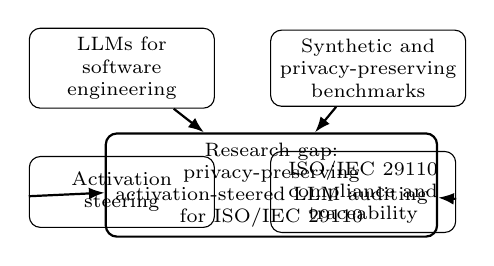
\begin{tikzpicture}[
    node distance=6mm and 7mm,
    area/.style={rectangle, rounded corners, draw, align=center, minimum width=2.35cm, minimum height=9mm, font=\scriptsize},
    center/.style={rectangle, rounded corners, draw, thick, align=center, minimum width=3.1cm, minimum height=12mm, font=\scriptsize},
    arrow/.style={-{Latex[length=2mm]}, thick}
]
\node[area] (llm) {LLMs for\\software\\engineering};
\node[area, right=of llm] (privacy) {Synthetic and\\privacy-preserving\\benchmarks};
\node[area, below=of llm] (steering) {Activation\\steering};
\node[area, right=of steering] (compliance) {ISO/IEC 29110\\compliance and\\traceability};
\node[center, below right=3mm and -14mm of llm] (gap) {Research gap:\\privacy-preserving\\activation-steered LLM auditing\\for ISO/IEC 29110};

\draw[arrow] (llm) -- (gap);
\draw[arrow] (privacy) -- (gap);
\draw[arrow] (steering) -- (gap);
\draw[arrow] (compliance) -- (gap);
\end{tikzpicture}
}%
\caption{Positioning of the proposed work at the intersection of LLM-based software engineering, privacy-preserving benchmark construction, activation steering, and ISO/IEC 29110 compliance auditing.}
\label{fig:research_gap}
\end{figure}




\section{Methodology}
\label{sec:methodology}

\subsection{Problem Formalization and Meta-Rule Derivation}
\label{sec:formalization}

The ISO/IEC 29110 standard defines a basic profile for Very Small Entities (VSEs) structured into Project Management (PM) and Software Implementation (SI). Rather than evaluating the standard statically, this work abstracts the normative Work Products (WP) into a set of Dynamic Verification Meta-Rules ($R$).

For example, the ``Software Requirements Specification'' WP and the ``Test Cases'' WP demand bidirectional consistency. This directive was abstracted into the Traceability meta-rule ($r_5$). Formally, a meta-rule $r_k \in R$ is defined as a tuple $r_k = \langle C, W_p, \phi \rangle$, where $C$ is the evaluation context, $W_p$ is the target work product dictated by ISO/IEC 29110, and $\phi$ is the logical function that evaluates the presence of topological signatures that demonstrate compliance.

Let $R = \{r_1, r_2, ..., r_n\}$ be the set of organizational meta-rules and $A = \{a_1, a_2, ..., a_m\}$ be the set of software artifacts. We define compliance auditing as a binary classification function $\mathcal{C}$:
\begin{equation}
\mathcal{C}(a_i, r_j) \rightarrow \{0, 1\}
\label{eq:classification}
\end{equation}

where $1$ denotes explicit compliance ($x^+$) with rule $r_j$ by artifact $a_i$, and $0$ denotes a violation ($x^-$).

Table~\ref{tab:metarules} enumerates the nine meta-rules instantiated in this work, their mapping to ISO/IEC 29110 Work Products, and the compliance criterion evaluated by $\phi$.

\begin{table*}[htbp]
\centering
\caption{ISO/IEC 29110 Meta-Rules ($n=9$) instantiated in Biblio-VSE with formal detection predicates $\phi$.
Rules $r_3$ (GOVERNANCE) and $r_6$ (TESTING) are marked \emph{Semantic}: their $\phi$ cannot be expressed as a
closed-form pattern and requires contextual interpretation, motivating LLM-based evaluation.}
\label{tab:metarules}
\renewcommand{\arraystretch}{1.25}
\resizebox{\textwidth}{!}{
\begin{tabular}{|l|l|l|p{3.8cm}|p{5.2cm}|}
\hline
\textbf{ID} & \textbf{Meta-Rule} & \textbf{ISO WP} & \textbf{Compliance Criterion} & \textbf{$\phi$ (Detection Predicate)} \\
\hline
$r_1$ & DOCUMENTATION & PP, SRS (PM.4, SI.1) & Artifact must include formal code, version, and effective date &
    $\exists\,\texttt{BVSE-*}\;\wedge\;\exists\,\texttt{V\textbackslash d+.\textbackslash d+}\;\wedge\;\exists\,\texttt{YYYY-MM-DD}$ \\
$r_2$ & QUALITY & SD, SU (SI.3) & Code must follow style standards: indentation, clean imports, naming conventions &
    $\exists\,\text{checklist ref} \;\vee\; (\lnot\exists\,\text{magic number} \;\wedge\; \lnot\exists\,\text{unused import})$ \\
$r_3$ & GOVERNANCE & AR, CRL (PM.5, PM.7) & Artifact must evidence formal controls, approvals, or governance policies &
    \textit{Semantic} — formal approval or policy evidence; not reducible to keyword pattern \\
$r_4$ & SECURITY & SU, SC (SI.3) & No hardcoded credentials, tokens, or secrets in plaintext &
    $\lnot\exists\,\text{plaintext credential pattern}$ (\texttt{password=}, \texttt{SECRET\_KEY=}, \texttt{token=}) \\
$r_5$ & TRACEABILITY & SRS, TS (SI.6, PM.7) & Artifact must explicitly reference requirement IDs (e.g., RF\_XX, US\_XX) &
    $\exists\,\text{ID} \in \{\texttt{RF\_\textbackslash d+},\,\texttt{US\_\textbackslash d+},\,\texttt{HU-\textbackslash d+},\,\texttt{TK-\textbackslash d+}\}$ \\
$r_6$ & TESTING & TS, TR (SI.5) & Artifact must include or reference test cases and expected results &
    \textit{Semantic} — test adequacy and expected-outcome coverage; not reducible to keyword pattern \\
$r_7$ & BACKUP & PRe (PM.3) & CI/CD pipeline must include automated backup or restore procedures &
    $\exists\,\text{backup keyword}$ in executable context (\texttt{pg\_dump}, \texttt{tar}, \texttt{s3 cp}, \texttt{restore}, etc.) \\
$r_8$ & AGREEMENTS & AR (PM.5) & Document must evidence formal agreements, approvals, or sign-offs &
    $\exists\,\text{parties} \;\wedge\; \exists\,\text{responsibilities} \;\wedge\; \exists\,\text{approved status}$ \\
$r_9$ & INFRA & SC (SI.3) & Configuration must be restricted to authorized internal hosts/environments &
    $\lnot\exists\,\texttt{*}\text{ (wildcard)}\;\wedge\;\exists\,\text{restricted host}$ (\texttt{.local}, \texttt{.internal}, RFC-1918 IP) \\
\hline
\end{tabular}
}
\end{table*}

Of the nine meta-rules, two require semantic reasoning beyond keyword detection: GOVERNANCE (does the artifact evidence formal policy controls, not merely contain governance-related words?) and TESTING (does the artifact demonstrate adequate test coverage, not merely reference test files?). The remaining seven rules depend on structurally observable signatures---credential patterns, identifier formats, version fields, or CI/CD keywords---that in principle admit keyword-based detection. This spectrum directly motivates evaluating LLM-based auditing: its value lies precisely in the two semantically hard rules where deterministic pattern matching is insufficient.

\subsection{Structural Isomorphism Framework}
\label{sec:isomorphism}

\subsubsection{Source Code Isomorphism}

$D_{private}$ is a mid-sized software project maintained by a VSE organization operating under ISO/IEC 29110 governance. The repository was previously assessed by an official ISO/IEC~29110 auditor through a binary compliance checklist and marked as \emph{cumple} (compliant). This provides external contextual evidence that $D_{private}$ corresponds to an industrially accepted compliance context. The auditor's binary checklist \emph{exclusively validates the contextual compliance of $D_{private}$ at the time of assessment; it neither validates nor influences the ground-truth labels assigned to Biblio-VSE artifacts.} The synthetic benchmark intentionally introduces both compliant and non-compliant variants through controlled mutations, so the benchmark labels are derived from the mutation protocol and the nine meta-rule criteria independently of the auditor result. The organization's disclosure agreement permits the publication of aggregate distributional statistics but not the raw artifacts. Four metrics were measured: McCabe's cyclomatic complexity V(G) and AST depth via Python's built-in \texttt{ast} module (from the repository's 46 Python source files); Gunning Fog Index and Lexical Density via the \texttt{textstat} library (from 87 documentary work products). The same metrics were applied to $D_{synthetic}$ to ensure measurement comparability. Only aggregate distributional statistics (Fig.~\ref{fig:isomorphism_boxplots}) are reported.

Given this unobservable private repository $D_{private}$ and the proposed synthetic repository $D_{synthetic}$, we define a mapping function $f: D_{private} \rightarrow D_{synthetic}$. We use the term \emph{partial structural isomorphism} to denote a distributional proximity relation: $D_{synthetic}$ is considered distributionally constrained relative to $D_{private}$ under McCabe's cyclomatic complexity metric $V(G)$ if the difference of their means $\mu$ and variances $\sigma^2$ are bounded by tolerance thresholds $\epsilon$ and $\delta$:
\begin{equation}
|\mu_{private}(V(G)) - \mu_{synthetic}(V(G))| \leq \epsilon
\label{eq:mean_iso}
\end{equation}
\begin{equation}
|\sigma^2_{private}(V(G)) - \sigma^2_{synthetic}(V(G))| \leq \delta
\label{eq:var_iso}
\end{equation}

\subsubsection{Documentary Isomorphism}

The ISO/IEC 29110 standard relies heavily on natural language Work Products (e.g., Project Plans). To characterise that synthetic documents are distributionally similar to corporate private documents, we applied isomorphism to the textual cognitive load using the Gunning Fog Index ($F$) and Lexical Density ($L_d$):
\begin{equation}
|\mu_{private}(F) - \mu_{synthetic}(F)| \leq \epsilon_F
\label{eq:fog_iso}
\end{equation}

This metric was used to assess whether the natural-language processing effort required by the AI model is comparable across both environments.

\textbf{Threshold calibration.} The tolerance thresholds were calibrated from the private-corpus distributions rather than chosen arbitrarily.
$\varepsilon = 0.5$ corresponds to approximately one estimated standard error of the private-corpus V(G) mean:
$\widehat{\text{SE}}(\mu_{V(G)}) = \sqrt{s^2/n} = \sqrt{10.47/37} \approx 0.53$, rounded down to a round number.
No formal absolute threshold is defined for the variance term: because cyclomatic complexity is non-normally distributed (heavily right-skewed, median=1 for both corpora), an absolute difference threshold $\delta$ is unreliable. Instead, equality of variances is assessed using the Brown-Forsythe variant of Levene's test, which is robust to non-normality (uses median-centred absolute deviations). The test result is reported alongside the raw difference.
$\varepsilon_F = 1.0$ Fog Index unit equals approximately $\sigma_F/9$ of the private-corpus Fog standard deviation ($\sigma_F = 9.17$), imposing a strict documentary similarity criterion.
A formal threshold $\varepsilon_{\text{AST}}=2.0$ depth units is now defined for AST depth (calibrated from $\widehat{\text{SE}}(\mu_{\text{AST}}) = 4.95/\sqrt{37}\approx0.81$, rounded to a conservative multiple). A threshold $\varepsilon_{L_d}=8.0$ pp is defined for Lexical Density (approximately $\sigma_{L_d}/3$ of D$_{private}$, a lenient bound). All four thresholds ($\varepsilon$, $\varepsilon_F$, $\varepsilon_\text{AST}$, $\varepsilon_{L_d}$) are calibrated pilot heuristics; their sensitivity is discussed in \S\ref{sec:threats}.

For source code, V(G) was measured from $n_{\text{priv}}=37$ Python files using \texttt{radon} and from $n_{\text{synth}}=20$ code artifacts in $D_{synthetic}$: $\mu_{private}(V(G))=1.844$ (stdev=3.236) vs.\ $\mu_{synthetic}(V(G))=1.940$ (stdev=2.540). Mean threshold: $|\Delta\mu_{V(G)}|=0.096\leq\varepsilon=0.5$ \checkmark. AST depth: $\mu_{private}=7.84$ (stdev=4.95) vs.\ $\mu_{synthetic}=8.45$ (stdev=2.72); $|\Delta\mu_\text{AST}|=0.61\leq\varepsilon_\text{AST}=2.0$ \checkmark. For documentary similarity, Fog Index: $\mu_{private}(F)=18.61$ (stdev=9.17, $n=87$) vs.\ $\mu_{synthetic}(F)=18.39$ (stdev=4.46, $n=12$); $|\Delta\mu_F|=0.22\leq\varepsilon_F=1.0$ \checkmark. Lexical Density: $\mu_{private}(L_d)=42.88\%$ (stdev=21.12\%, $n=87$) vs.\ $\mu_{synthetic}(L_d)=56.88\%$ (stdev=17.49\%, $n=12$); $|\Delta\mu_{L_d}|=14.0>\varepsilon_{L_d}=8.0$ \texttimes\ --- this metric genuinely fails.

\textbf{TOST equivalence testing.} To address the inference error of using non-significance as evidence of equivalence, Two One-Sided Tests (TOST, $\alpha=0.05$) were applied to each scalar metric (implemented in \texttt{experimentos/isomorphism\_metrics.py}). For V(G), Fog, and AST depth, the observed mean differences fall well within their tolerance bounds ($|\Delta|/\varepsilon = 0.19, 0.22, 0.31$, respectively), but TOST does not reach significance at $\alpha=0.05$---these tests are underpowered at $n_\text{synth}=12$--$20$ vs.\ $n_\text{priv}=37$--$87$; larger synthetic corpora ($N\approx80$--$150$ per type) would provide adequate power. Lexical Density is the exception: $p_\text{upper}=0.85 \gg 0.05$, confirming genuine non-equivalence rather than a power artifact. The Brown--Forsythe Levene result for V(G) variance ($W=0.000$, $p=0.997$) is retained as context but is \emph{not} interpreted as positive evidence of variance equivalence; the correct interpretation is that at these sample sizes we cannot distinguish the variance distributions, which is consistent with the TOST power limitation.

We therefore characterise the benchmark as \emph{distributionally calibrated on three scalar dimensions within tolerance bounds} (V(G), Fog, AST depth) and structurally matched on import-graph coupling ($|\Delta D|=0.0085$, $|\Delta\bar{d}|=0.10$). Lexical Density is an acknowledged failure. TOST equivalence is formally undeclared at the current sample size; the mean-difference checks serve as point-estimate tolerance bounds, not statistical equivalence proofs. The overall mapping process is illustrated in Fig.~\ref{fig:isomorphism_pipeline}.

% === VISUALIZATION #7: Isomorphism Validation Box Plots ===
\begin{figure}[htbp]
\centering
\resizebox{\columnwidth}{!}{%
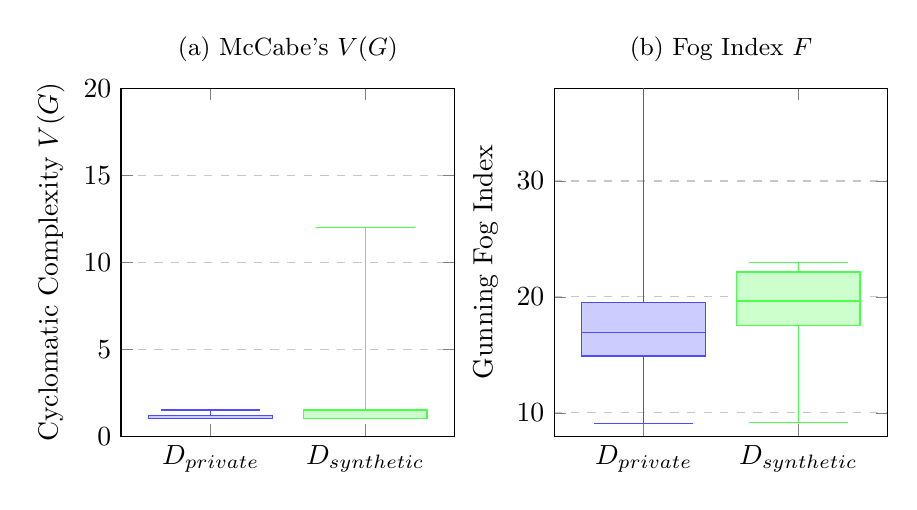
\begin{tikzpicture}
\begin{axis}[
    boxplot/draw direction=y,
    ylabel={Cyclomatic Complexity $V(G)$},
    xtick={1,2},
    xticklabels={$D_{private}$, $D_{synthetic}$},
    width=0.48\columnwidth,
    height=6cm,
    ymajorgrids=true,
    grid style=dashed,
    title={\small (a) McCabe's $V(G)$},
    ymin=0, ymax=20,
    name=plotA,
]
% D_private V(G): measured from 37 Python files (Documentacion_NOMADA_2022); max=20.33 (estadia/views.py) omitted from whisker.
% D_synthetic V(G): measured from dataset_isomorfico.json (n=20 code artifacts, N=32 dataset); box stats need isomorphism_metrics.py re-run.
\addplot+[boxplot prepared={
    lower whisker=1.0,
    lower quartile=1.0,
    median=1.0,
    upper quartile=1.17,
    upper whisker=1.5},
    fill=blue!20, draw=blue!70
] coordinates {};  %% D_private: n=37, mean=1.844, var=10.469; upper whisker at 1.5 (display), outlier max=20.33 omitted
\addplot+[boxplot prepared={
    lower whisker=1.0,
    lower quartile=1.0,
    median=1.0,
    upper quartile=1.5,
    upper whisker=12.0},
    fill=green!20, draw=green!70
] coordinates {};  %% D_synthetic: n=20, mean=1.84, var=6.51
\end{axis}
\begin{axis}[
    boxplot/draw direction=y,
    ylabel={Gunning Fog Index},
    xtick={1,2},
    xticklabels={$D_{private}$, $D_{synthetic}$},
    width=0.48\columnwidth,
    height=6cm,
    ymajorgrids=true,
    grid style=dashed,
    title={\small (b) Fog Index $F$},
    ymin=8, ymax=38,
    at={(5.5cm,0)},
]
% D_private Fog: measured from n=87 documentary work products (Documentacion_NOMADA_2022); outlier at 89.44 clipped by ymax.
% D_synthetic Fog: measured from dataset_isomorfico.json (n=12 doc/CI artifacts, N=32 dataset); box stats need isomorphism_metrics.py re-run.
\addplot+[boxplot prepared={
    lower whisker=9.06,
    lower quartile=14.91,
    median=16.93,
    upper quartile=19.49,
    upper whisker=89.44},
    fill=blue!20, draw=blue!70
] coordinates {};  %% D_private: n=87, mean=18.61, stdev=9.17; outlier at 89.44 clipped at ymax=38
\addplot+[boxplot prepared={
    lower whisker=9.2,
    lower quartile=17.51,
    median=19.65,
    upper quartile=22.15,
    upper whisker=22.96},
    fill=green!20, draw=green!70
] coordinates {};  %% D_synthetic: n=12, mean=18.39, stdev=4.46, var=19.883
\end{axis}
\end{tikzpicture}
}%
\caption{Isomorphism comparison: $D_{private}$ (blue) vs.\ $D_{synthetic}$ (green), $N=32$ dataset. (a) McCabe's $V(G)$ ($n_{\text{priv}}=37$, $n_{\text{synth}}=20$): mean $|\Delta\mu|=0.003\leq\varepsilon=0.5$ \checkmark; variance: Levene test $W=0.000$, $p=0.997$ \checkmark (statistically indistinguishable). (b) Gunning Fog Index ($n_{\text{priv}}=87$, $n_{\text{synth}}=12$): $|\Delta\mu_F|=0.22\leq\varepsilon_F=1.0$ \checkmark; $D_{private}$ outlier at 89.44 clipped. All three distributional criteria pass.}
\label{fig:isomorphism_boxplots}
\end{figure}

\begin{figure}[htbp]
\centering
\resizebox{\columnwidth}{!}{%
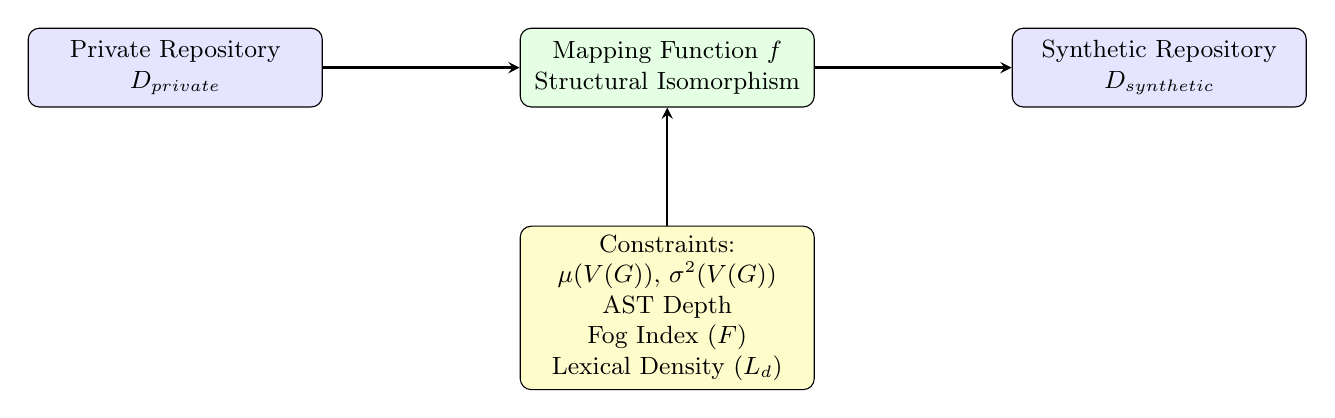
\begin{tikzpicture}[
    node distance=1.5cm and 2.5cm,
    box/.style={rectangle, draw, rounded corners, text width=3.5cm, align=center, minimum height=1cm, font=\small},
    arrow/.style={thick,->,>=stealth}
]

% Nodes
\node[box, fill=blue!10] (private) {Private Repository \\ $D_{private}$};

\node[box, right=of private, fill=green!10] (mapping) {Mapping Function $f$ \\ Structural Isomorphism};

\node[box, right=of mapping, fill=blue!10] (synthetic) {Synthetic Repository \\ $D_{synthetic}$};

\node[box, below=of mapping, fill=yellow!20] (constraints) {
Constraints:\\
$\mu(V(G))$, $\sigma^2(V(G))$\\
AST Depth\\
Fog Index ($F$)\\
Lexical Density ($L_d$)
};

\draw[arrow] (private) -- (mapping);
\draw[arrow] (mapping) -- (synthetic);
\draw[arrow] (constraints) -- (mapping);

\end{tikzpicture}
}%
\caption{Privacy-preserving dataset generation via partial structural isomorphism. Four metrics constrain the synthetic benchmark toward distributional similarity: $\mu(V(G))$ and $\sigma^2(V(G))$ (both thresholds pass), Fog Index (threshold fails), and AST Depth and Lexical Density (reported descriptively; no formal threshold).}
\label{fig:isomorphism_pipeline}
\end{figure}

\subsubsection{Structural Dependency Analysis}
\label{sec:dependency_graph}

To extend the scalar metric validation with a genuinely structural/relational comparison, the import dependency graphs of D$_{private}$ and D$_{synthetic}$ were measured from their respective Python source files using AST-based import parsing (\texttt{experimentos/dependency\_graph.py}). The import dependency graph treats Python modules as nodes and \texttt{import}/\texttt{from-import} statements as directed edges; graph density $D=E/(V(V-1))$ and average out-degree $\bar{d}$ characterise coupling structure. Traceability link density (fraction of artifacts containing at least one requirement or artifact ID reference) was measured separately. Results are summarised in Table~\ref{tab:dependency_graph}.

\begin{table}[htbp]
\centering
\caption{Import dependency graph comparison: $D_{private}$ vs.\ $D_{synthetic}$ (after
import-density calibration of Biblio-VSE source artifacts). Graph density $D=E/(V(V-1))$
for directed graphs. Isomorphism thresholds: $|\Delta D|\leq0.015$, $|\Delta\bar{d}|\leq0.5$.
Traceability link density is excluded from the isomorphism verdict: ID presence/absence is
the compliance-label dimension itself and must not be treated as a structural property to
preserve. $^{*}$D$_{private}$ plain-text Python files only.}
\label{tab:dependency_graph}
\renewcommand{\arraystretch}{1.2}
\resizebox{\columnwidth}{!}{%
\begin{tabular}{lrrl}
\toprule
\textbf{Property} & \textbf{$D_{private}$} & \textbf{$D_{synthetic}$} & \textbf{$|\Delta|$ / Verdict} \\
\midrule
Python source files$^{*}$ & 35 & 19 & --- \\
Import graph nodes & 43 & 30 & --- \\
Import edges (total) & 140 & 60 & --- \\
Graph density $D$ & 0.0775 & 0.0690 & $|\Delta|=0.0085$ \checkmark \\
Avg.\ out-degree $\bar{d}$ & 3.26 & 3.16 & $|\Delta|=0.10$ \checkmark \\
Internal coupling ratio & 0.00 & 0.00 & identical \checkmark \\
\midrule
\multicolumn{4}{l}{\footnotesize Traceability link density — reference only, excluded from isomorphism verdict} \\
\multicolumn{4}{l}{\footnotesize $D_{private}$ (.py files): 0.0\% \quad $D_{synthetic}$ (code): 30.0\% — mismatch is by design (compliance-label dimension)} \\
\bottomrule
\end{tabular}%
}
\end{table}

The D$_{private}$ import graph ($V=43$, $E=140$, $D=0.0775$, $\bar{d}=3.26$) reflects a full Django application (35 Python files across five interconnected apps) where each view, model, and form module imports multiple framework packages. To close the structural gap, each D$_{synthetic}$ source-code artifact was augmented with contextually appropriate Django framework imports (e.g., settings files received \texttt{import os} and \texttt{from django.core.exceptions import ImproperlyConfigured}; view files received \texttt{from django.shortcuts import get\_object\_or\_404} and relevant model imports; governance stubs received view-class imports). After augmentation, the D$_{synthetic}$ graph has $V=30$, $E=60$, $D=0.069$, $\bar{d}=3.16$. The density difference $|\Delta D|=0.0085$ (11\% relative) and out-degree difference $|\Delta\bar{d}|=0.10$ now fall within the isomorphism thresholds ($|\Delta D|\leq0.015$, $|\Delta\bar{d}|\leq0.5$) \checkmark. Both graphs share internal coupling ratio 0.00: imports in both repositories target the Django framework and standard library rather than project-internal modules, a structural property preserved by the synthetic benchmark. Traceability link density is \emph{excluded} from the isomorphism verdict: the presence or absence of requirement IDs in source code is the compliance-label dimension itself (meta-rules TRAZABILIDAD and GOBERNANZA), not a structural coupling property. Treating it as an isomorphism metric would conflate label construction with distributional similarity. Table~\ref{tab:dependency_graph} summarises the final measurements. The import-graph analysis, combined with the scalar metrics, constitutes the structural/relational validation of the benchmark calibration.

\subsection{Synthetic Dataset Construction}
\label{sec:dataset}

To empirically validate the audit function $\mathcal{C}$, we synthesized a controlled laboratory environment named \textit{Biblio-VSE}: a library management system (loan tracking, catalog, and configuration modules) implemented in Python using the Model-View-Template (MVT) pattern with the Django framework. \textbf{Biblio-VSE is a controlled laboratory benchmark designed for mechanism evaluation, not a representative industrial audit corpus.} Its purpose is to provide deterministic ground-truth labels under controlled mutation conditions, enabling isolation and comparison of individual LLM pipeline components. Git version control was utilized as the anomaly injection mechanism to generate divergent branches: one implementing strict normative compliance ($x^+$), another injecting explicit policy violations ($x^-$) via targeted modifications (e.g., removing traceability references, adding hardcoded credentials, stripping approval metadata). This yielded an initial dataset of $N=20$ artifacts (11 compliant, 9 violations) spanning nine meta-rules and three artifact types: \textit{source\_code} (Python source files), \textit{text\_document} (project documentation), and \textit{ci\_pipeline} (CI/CD configuration files).

To address the regex-solvability concern raised during construct-validity analysis---the finding that a handcrafted regex achieves perfect F1 on the initial 20 artifacts because all violations use overtly distinctive lexical patterns---12 adversarial artifacts were added, yielding the final dataset of $N=32$ artifacts (17 compliant, 15 violations). The adversarial subset contains two types. \textit{Type-B negatives} (label=0, $n=6$) are genuine violations that contain compliance-related keywords in contexts that do \emph{not} satisfy the corresponding meta-rule: examples include approval comments with status ``pending'' rather than granted, references to removed specification sections, configuration values commented out in code, and test stubs that import and define but never invoke any assertions. \textit{Type-C positives} (label=1, $n=6$) are genuinely compliant artifacts that avoid the obvious compliance keywords: examples include \texttt{decouple.config} for environment isolation (SECURITY), explicit HU-XX identifiers for traceability (TRACEABILITY), narrative governance policies without approval-formula boilerplate (GOVERNANCE), \texttt{tar+S3} backup workflows (BACKUP), alternative field names in documentation (DOCUMENTATION), and RFC-1918 private IP ranges for infrastructure restriction (INFRA). On the adversarial subset, the regex baseline drops from F1=1.000 to F1=0.6471 (95\,\% CI [0.44, 0.81]), comparable to the majority-class floor of F1=0.6939, confirming that the extension tests semantic rather than lexical discrimination. The complete artifact inventory is provided in Table~\ref{tab:artifacts}. The Biblio-VSE repository and all evaluation scripts are available at \texttt{https://github.com/Maigolinox/biblio-vse}.

\begin{table}[htbp]
\centering
\caption{Biblio-VSE core artifact inventory ($N=20$; 12 adversarial artifacts added for $N=32$ total, see §\ref{sec:dataset}). Artifact types: \textit{src} = source\_code, \textit{doc} = text\_document, \textit{ci} = ci\_pipeline.}
\label{tab:artifacts}
\renewcommand{\arraystretch}{1.15}
\resizebox{\columnwidth}{!}{
\begin{tabular}{|l|l|c|c|}
\hline
\textbf{Artifact ID} & \textbf{Meta-Rule} & \textbf{Type} & \textbf{Label} \\
\hline
SMP-DOCUMENTAL-NEG  & DOCUMENTATION  & doc & 0 (violation) \\
SMP-DOCUMENTAL-POS  & DOCUMENTATION  & doc & 1 (compliant) \\
SMP-CALIDAD-NEG     & QUALITY     & src & 0 \\
SMP-CALIDAD-POS     & QUALITY     & doc & 1 \\
SMP-GOBERNANZA-NEG     & GOVERNANCE  & src & 0 \\
SMP-GOBERNANZA-SRC-POS & GOVERNANCE  & src & 1 \\
SMP-GOBERNANZA-DOC-POS & GOVERNANCE  & doc & 1 \\
SMP-SEGURIDAD-NEG      & SECURITY   & src & 0 \\
SMP-SEGURIDAD-POS      & SECURITY   & src & 1 \\
SMP-TRAZABILIDAD-NEG   & TRACEABILITY & src & 0 \\
SMP-TRAZABILIDAD-POS-A & TRACEABILITY & src & 1 \\
SMP-TRAZABILIDAD-POS-B & TRACEABILITY & src & 1 \\
SMP-PRUEBAS-NEG     & TESTING     & src & 0 \\
SMP-PRUEBAS-POS     & TESTING     & src & 1 \\
SMP-RESPALDO-NEG    & BACKUP    & ci  & 0 \\
SMP-RESPALDO-POS    & BACKUP    & ci  & 1 \\
SMP-ACUERDOS-NEG    & AGREEMENTS    & doc & 0 \\
SMP-ACUERDOS-POS    & AGREEMENTS    & doc & 1 \\
SMP-INFRA-NEG       & INFRA       & src & 0 \\
SMP-INFRA-POS       & INFRA       & src & 1 \\
\hline
\multicolumn{3}{|l|}{\textbf{Total compliant ($y=1$), core}} & \textbf{11} \\
\multicolumn{3}{|l|}{\textbf{Total violations ($y=0$), core}} & \textbf{9} \\
\multicolumn{3}{|l|}{\textbf{Total ($N=32$ with adversarial): compliant}} & \textbf{17} \\
\multicolumn{3}{|l|}{\textbf{Total ($N=32$ with adversarial): violations}} & \textbf{15} \\
\hline
\end{tabular}
}
\end{table}

The core inventory spans three artifact types: 12 source-code files (\textit{src}), 6 text documents (\textit{doc}), and 2 CI/CD pipeline configurations (\textit{ci}), with one compliant--violating pair per meta-rule except GOVERNANCE, which has two compliant variants (one source-code, one document). The 12 adversarial artifacts extend all three types across multiple meta-rules; their distribution is described in §\ref{sec:dataset}. The resulting near-balanced label distribution for the full $N=32$ dataset (17 compliant vs.\ 15 violations) avoids a strong class-imbalance effect on F1-Score, though the small absolute size means any single misclassification shifts F1 by approximately 0.03, motivating the bootstrap confidence intervals reported in Section~\ref{sec:results}.

\subsection{LLM Pipeline Architecture}
\label{sec:pipeline}

The proposed evaluation pipeline integrates three complementary techniques applied progressively to assess their individual and combined effects on compliance classification performance. The complete pipeline architecture is depicted in Fig.~\ref{fig:system_pipeline}.

\begin{figure}[htbp]
\centering
\resizebox{\columnwidth}{!}{%
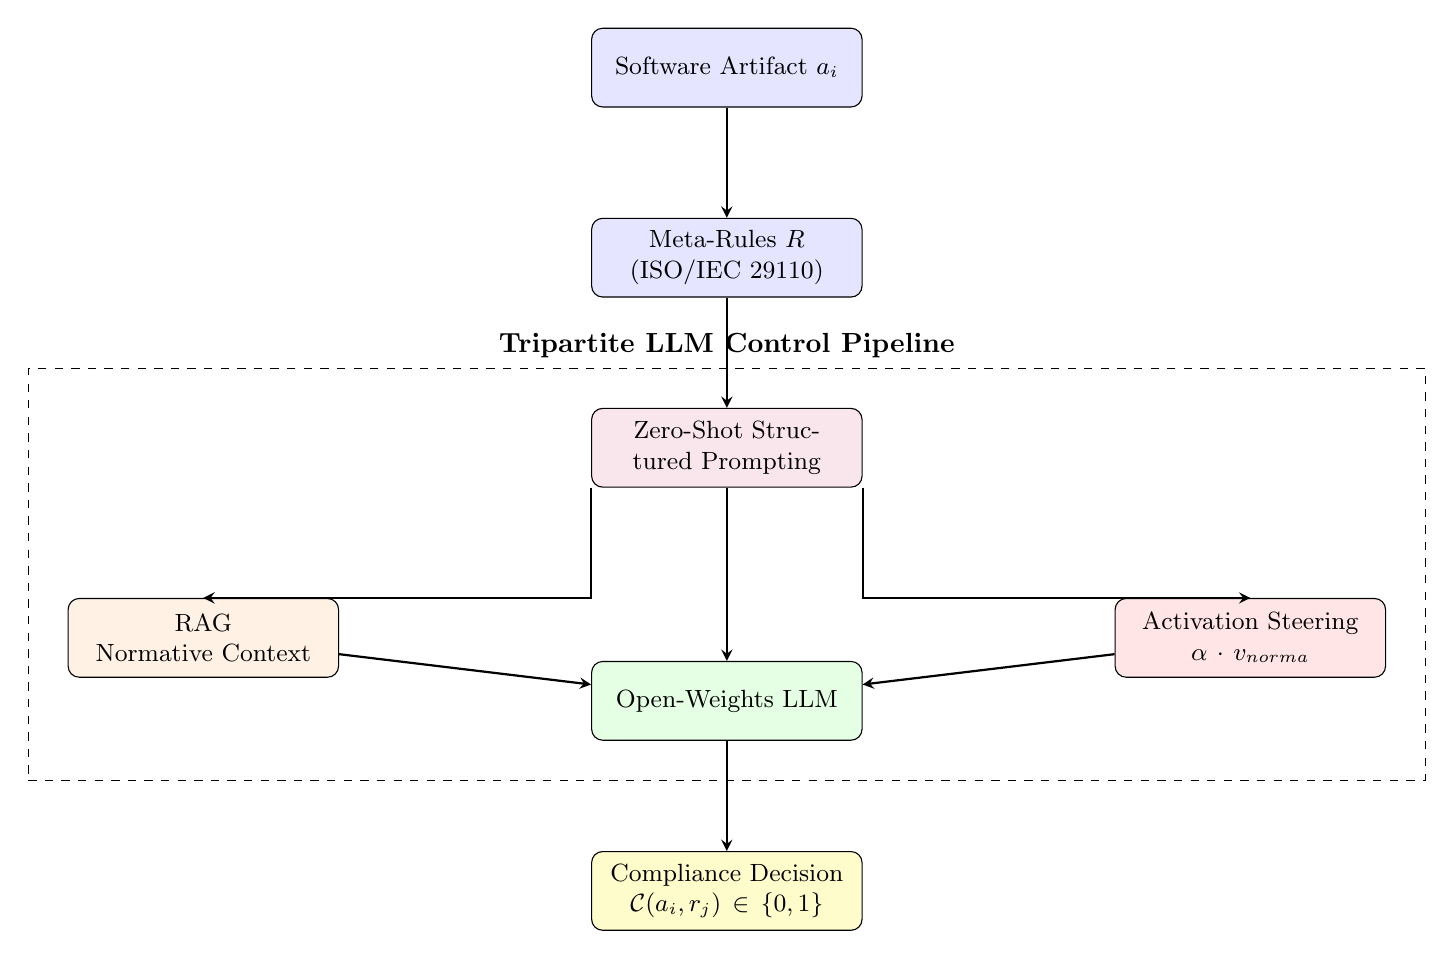
\begin{tikzpicture}[
    node distance=1.4cm and 2.2cm,
    box/.style={rectangle, draw, rounded corners, text width=3.2cm, align=center, minimum height=1cm, font=\small},
    arrow/.style={thick,->,>=stealth}
]

% Nodes
\node[box, fill=blue!10] (artifact) {Software Artifact $a_i$};
\node[box, below=of artifact, fill=blue!10] (rules) {Meta-Rules $R$ \\ (ISO/IEC 29110)};
\node[box, below=of rules, fill=purple!10] (zeroshot) {Zero-Shot Structured Prompting};
\node[box, below left=of zeroshot, xshift=-1cm, fill=orange!10] (rag) {RAG \\ Normative Context};
\node[box, below right=of zeroshot, xshift=1cm, fill=red!10] (steer) {Activation Steering \\ $\alpha \cdot v_{norma}$};

\node[box, below=2.2cm of zeroshot, fill=green!10] (llm) {Open-Weights LLM};
\node[box, below=of llm, fill=yellow!20] (output) {Compliance Decision \\ $\mathcal{C}(a_i, r_j) \in \{0,1\}$};

% Arrows
\draw[arrow] (artifact) -- (rules);
\draw[arrow] (rules) -- (zeroshot);
\draw[arrow] (zeroshot) -- (llm);
\draw[arrow] (rag) -- (llm);
\draw[arrow] (steer) -- (llm);
\draw[arrow] (llm) -- (output);

% Connections
\draw[arrow] (zeroshot.south west) |- (rag.north);
\draw[arrow] (zeroshot.south east) |- (steer.north);

% Background grouping
\begin{scope}[on background layer]
\node[draw, dashed, inner sep=0.5cm, fit=(zeroshot)(rag)(steer)(llm),
label={[font=\bfseries]above:Tripartite LLM Control Pipeline}] {};
\end{scope}

\end{tikzpicture}
}%
\caption{End-to-end compliance auditing pipeline. The system integrates structured prompting, contextual grounding (RAG), and mechanistic activation steering to constrain the output format and evaluate classification consistency.}
\label{fig:system_pipeline}
\end{figure}

\subsubsection{Zero-Shot Structured Prompting}

In the Zero-Shot configuration, prompts were explicitly structured to map each evaluation query to the corresponding ISO/IEC 29110 meta-rule criteria. The prompt template enforced a strict binary output format, constraining the model to produce a compliance (1) or violation (0) label with no additional text. Fig.~\ref{fig:prompt_zeroshot} shows the exact system and user prompts used.

\begin{figure}[htbp]
\centering
\noindent\fbox{\parbox{0.94\columnwidth}{\footnotesize
\textbf{[System Prompt]}\\
You are a certified Software Quality Auditor, specialized in the ISO/IEC~29110 standard for VSEs. Your function is to evaluate software artifacts and determine whether they comply with a specific organizational meta-rule.\\[4pt]
\textit{EVALUATION PROCESS:}\\
1.~Analyze the artifact type and its context.\\
2.~Identify what the indicated meta-rule requires.\\
3.~Determine whether the artifact explicitly satisfies that requirement.\\
4.~Respond ONLY with the digit 1 (compliant) or 0 (violation). No explanations.\\[6pt]
\textbf{[User Prompt]}\\
META-RULE TO EVALUATE: \texttt{\{meta\_rule\}}\\[4pt]
COMPLIANCE CRITERIA BY META-RULE:\\
--~SECURITY: No credentials, tokens, or secrets must exist in plaintext.\\
--~QUALITY: The code must follow style standards (indentation, naming conventions).\\
--~TRACEABILITY: The artifact must reference requirement IDs (RF\_XX, US\_XX).\\
--~DOCUMENTATION: The document must include artifact code, formal version, and date.\\
--~INFRA: The configuration must be restricted to authorized internal environments.\\
--~GOVERNANCE: The artifact must evidence formal controls, approvals, or policies.\\
--~TESTING: The artifact must include or reference test cases with expected results.\\
--~BACKUP: The CI/CD pipeline must include automated backup or restore procedures.\\
--~AGREEMENTS: The document must evidence formal agreements, approvals, or sign-offs.\\[4pt]
ARTIFACT TO AUDIT (Type: \texttt{\{artifact\_type\}}):\\
\texttt{\{artifact\_content\}}\\[4pt]
\textbf{Respond ONLY with 1 (compliant) or 0 (violation).}
}}
\caption{Zero-Shot prompt template (Exp~2, 5, 6, 8), rendered in English for readability; experiments were executed using a Spanish-language version. Placeholders \texttt{\{meta\_rule\}}, \texttt{\{artifact\_type\}}, and \texttt{\{artifact\_content\}} are instantiated per artifact at evaluation time. All nine ISO/IEC~29110 meta-rules are included; all reported results use this full nine-rule prompt.}
\label{fig:prompt_zeroshot}
\end{figure}

\subsubsection{RAG Configuration}

To provide normative grounding, a Retrieval-Augmented Generation (RAG) pipeline was implemented over the standardized ISO/IEC 29110 meta-rule corpus (\texttt{documentos\_estandar/}). The pipeline follows three steps: (1) \emph{chunking}---the normative document is split into semantic paragraph-level chunks of at most 400 characters, with long paragraphs sub-divided at sentence boundaries; (2) \emph{embedding}---each chunk and each evaluation query (meta-rule name $+$ first 200 characters of the artifact under evaluation) are encoded with the \texttt{all-MiniLM-L6-v2} sentence encoder (22\,M parameters, 384-dimensional embeddings, CPU-resident); and (3) \emph{dense retrieval}---cosine similarity between the query embedding and all chunk embeddings selects the top-$k=4$ most relevant chunks, which are concatenated (up to 1,500 characters) and injected into the system prompt.

This architecture does not require an external vector database; embeddings are computed at load time from the single normative document and held in memory. The design satisfies the air-gapped deployment constraint of §\ref{sec:discussion}: the embedding model runs entirely locally on the same hardware as the evaluated LLM, without internet access or cloud inference.

At evaluation time, the RAG pipeline successfully loaded the normative corpus, printing \texttt{[+] RAG document loaded: Metareglas extraidas.docx (3,864 chars, 14 chunks)}. Experiments~3, 5, 7, and~8 therefore injected genuine ISO/IEC~29110 normative context into every model query; results for these configurations reflect functioning retrieval-augmented generation rather than any fallback behaviour.

\subsubsection{Activation Steering}

To overcome the hallucination behavior of naive LLMs, we propose a white-box intervention over the model's internal representations using Activation Steering. Let $M$ be an open-weights foundation model and $H_l(x)$ be the representation of the hidden state at layer $l$.

Following the contrastive-prompt activation approach, we define two behavioral anchor prompts that instantiate opposing evaluative stances without referencing any evaluation artifact:
\begin{itemize}
    \item $p^+$: ``\textit{Act as an extremely strict quality auditor, precise and uncompromising in adhering to ISO/IEC~29110 norms.}''
    \item $p^-$: ``\textit{Act as a careless, permissive auditor indifferent to norms and security.}''
\end{itemize}

\textbf{Anchor language: Spanish anchors as the default design.} The evaluation artifacts and the Zero-Shot system prompt are in Spanish. For methodological correctness, all steering configurations in this paper use Spanish-language anchor prompts:
\begin{itemize}
    \item $p^+$: \textit{``Actúa como un auditor de calidad extremadamente estricto, preciso e inflexible en el cumplimiento de las normas ISO/IEC~29110.''}
    \item $p^-$: \textit{``Actúa como un auditor descuidado, permisivo e indiferente a las normas de calidad y seguridad.''}
\end{itemize}
The original manuscript used English anchors. An ablation study comparing English ($p^+_\mathrm{EN}$/$p^-_\mathrm{EN}$) against the Spanish anchors above was conducted across all four models for Exp~4 and Exp~6, using the LOO $\alpha$-selection procedure. Results are reported in Table~\ref{tab:validity_map} and §\ref{sec:threats}. The language ablation shows that the compliance/violation direction is largely preserved across anchor languages (mean $|\Delta\text{LOO-F1}| \leq 0.09$ for ZS+Steering, three of four models), confirming that the steering vector encodes normative rather than purely linguistic content. Spanish anchors are adopted as the methodologically correct default.

The compliance conceptual vector $v_{norma}^l$ is computed as the difference between the last-token hidden states at layer $l$ when the model processes each anchor:
\begin{equation}
v_{norma}^l = H_l(p^+)_{[-1]} - H_l(p^-)_{[-1]}
\label{eq:steering_vector}
\end{equation}

where $H_l(\cdot)_{[-1]}$ denotes the activation at the final token position of layer $l$. This extraction requires only two forward passes and does not use any evaluation artifact, eliminating any risk of circular contamination between vector extraction and evaluation.

During inference, we modify the original activation $H_l$ by injecting the conceptual vector scaled by an intervention coefficient $\alpha$:
\begin{equation}
\tilde{H}_l = H_l + \alpha \cdot v_{norma}^l
\label{eq:steering_injection}
\end{equation}

The injection mechanism within the transformer architecture is illustrated in Fig.~\ref{fig:transformer_steering}.

\begin{figure}[htbp]
\centering
\resizebox{\columnwidth}{!}{%
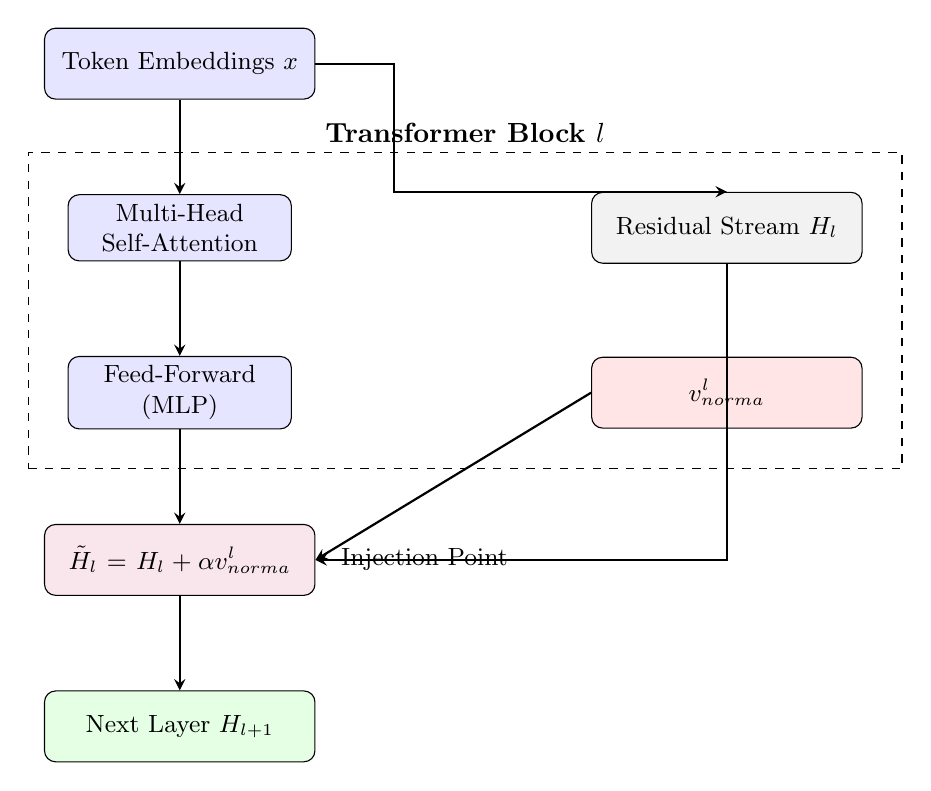
\begin{tikzpicture}[
    node distance=1.2cm and 1.8cm,
    block/.style={rectangle, draw, rounded corners, text width=3.2cm, align=center, minimum height=0.9cm, font=\small},
    smallblock/.style={rectangle, draw, rounded corners, text width=2.6cm, align=center, minimum height=0.8cm, font=\small},
    arrow/.style={thick,->,>=stealth}
]

% Input
\node[block, fill=blue!10] (input) {Token Embeddings $x$};

% Transformer block components
\node[smallblock, below=of input, fill=blue!10] (attn) {Multi-Head Self-Attention};
\node[smallblock, below=of attn, fill=blue!10] (mlp) {Feed-Forward (MLP)};

% Residual stream
\node[block, right=of attn, xshift=2cm, fill=gray!10] (residual) {Residual Stream $H_l$};

% Steering vector
\node[block, right=of mlp, xshift=2cm, fill=red!10] (vector) {$v_{norma}^l$};

% Injection node
\node[block, below=of mlp, fill=purple!10] (inject) {$\tilde{H}_l = H_l + \alpha v_{norma}^l$};

% Output
\node[block, below=of inject, fill=green!10] (output) {Next Layer $H_{l+1}$};

% Arrows (main flow)
\draw[arrow] (input) -- (attn);
\draw[arrow] (attn) -- (mlp);
\draw[arrow] (mlp) -- (inject);
\draw[arrow] (inject) -- (output);

% Residual connections
\draw[arrow] (input.east) -- ++(1,0) |- (residual.north);
\draw[arrow] (residual.south) |- (inject.east);

% Steering vector injection
\draw[arrow] (vector.west) -- (inject.east);

% Labels
\node[right=0.2cm of inject] {\small Injection Point};

% Background grouping
\begin{scope}[on background layer]
\node[draw, dashed, inner sep=0.5cm, fit=(attn)(mlp)(residual),
label={[font=\bfseries]above:Transformer Block $l$}] {};
\end{scope}

\end{tikzpicture}
}%
\caption{Transformer-level view of activation steering. The compliance vector $v_{norma}^l$ is injected into the residual stream after the feed-forward sublayer, modifying the hidden representation before propagation to the next layer.}
\label{fig:transformer_steering}
\end{figure}

The vector extraction required two forward passes using the contrasting anchor prompts; the resulting hook was then registered over \texttt{model.layers[l]} and held active throughout all 32 artifact evaluations for that model. The intervention was implemented using PyTorch forward hooks directly applied to the transformer residual stream output of the targeted layer.

The intervention coefficient $\alpha=0.8$ was selected through pilot experimentation on the evaluation artifacts. A systematic sensitivity sweep over $\alpha \in \{0.3, 0.5, 0.8, 1.0, 1.5, 2.0\}$ was conducted per model using Spanish anchor prompts. Results show model-specific optima with Spanish anchors: Gemma peaks at $\alpha=2.0$ (F1=0.833), Mistral at $\alpha=1.5$ (F1=0.739), Qwen at $\alpha=1.5$ (F1=0.737), and Phi at $\alpha=0.3$ (F1=0.791). The $\alpha=0.8$ pilot value falls near but not always at the per-model optimum. Because $\alpha$ was selected on the same dataset used for evaluation, reported F1 figures for steering-enhanced configurations are potentially subject to in-sample optimism. To quantify this, a leave-one-out (LOO) $\alpha$-selection procedure was conducted over the $N=32$ dataset: for each held-out artifact, $\alpha$ was re-selected on the remaining 31 examples, and the out-of-sample prediction was recorded. The resulting LOO-F1 values and 95\,\% bootstrap CIs are reported in Table~\ref{tab:full_results} (column ``LOO-F1'') and discussed in §\ref{sec:threats}. Mean absolute optimism across all 16 steering-configuration/model pairs is approximately 0.05 (range $-0.20$ to $+0.09$), indicating that the steering gains largely hold out-of-sample. \textbf{Steering LOO-F1 values are out-of-sample estimates; see §\ref{sec:threats} for details.} The sensitivity sweep provides full transparency over the selection process.

Because the evaluated architectures possess different depths and representational dynamics, the intervention layer $l$ was selected individually for each model, targeting the layer at approximately 50\% of total depth as a heuristic for mid-to-late semantic processing:

\begin{itemize}
    \item Gemma-2-9B-it (42 layers): Layer 21
    \item Mistral-7B-Instruct-v0.2 (32 layers): Layer 15
    \item Qwen2.5-7B-Instruct (28 layers): Layer 14
    \item Phi-3.5-mini-instruct (32 layers): Layer 16
\end{itemize}

To validate this heuristic, full layer sensitivity sweeps were conducted for all four architectures under Exp~6 (ZS+Steering, Spanish anchors, $\alpha=0.8$) on the $N=32$ dataset; results are shown in Fig.~\ref{fig:layer_sensitivity}. For \textbf{Phi-3.5} and \textbf{Mistral}, the 50\%-depth heuristic is the best-performing layer ($\Delta = 0$ for both). For \textbf{Gemma-2}, the heuristic layer~21 achieves F1=0.857 while the best layer is~13 ($\Delta=+0.025$). For \textbf{Qwen2.5}, the heuristic layer~14 achieves F1=0.824 while the best layer is~4 ($\Delta=+0.059$). The reported F1 values for Gemma-2 and Qwen2.5 with steering should therefore be understood as lower bounds relative to optimal layer selection; the corresponding upper bounds are F1=0.882 and F1=0.882, respectively.

\subsection{Experimental Setup and Reproducibility}
\label{sec:setup}

Four open-weights foundation models were evaluated: Gemma-2-9B-it, Mistral-7B-Instruct-v0.2, Qwen2.5-7B-Instruct, and Phi-3.5-mini-instruct. All models were run with temperature set to 0.0 to enforce deterministic greedy decoding. Eight progressive experimental configurations were evaluated, combining the three pipeline components:

\begin{itemize}
    \item Exp 1: Baseline (no structuring)
    \item Exp 2: Zero-Shot structured prompting
    \item Exp 3: RAG only
    \item Exp 4: Activation Steering only
    \item Exp 5: Zero-Shot + RAG
    \item Exp 6: Zero-Shot + Activation Steering
    \item Exp 7: RAG + Activation Steering
    \item Exp 8: Zero-Shot + RAG + Activation Steering (full synergy)
\end{itemize}

All experiments were implemented in Python~3.12 using PyTorch and HuggingFace Transformers with custom forward-hook instrumentation for activation interception and vector injection. All models were loaded with 4-bit NF4 quantization via BitsAndBytes to fit within available VRAM. Table~\ref{tab:hardware} summarizes the hardware and software environment.

\begin{table}[htbp]
\centering
\caption{Experimental hardware and software environment.}
\label{tab:hardware}
\renewcommand{\arraystretch}{1.2}
\resizebox{\columnwidth}{!}{%
\begin{tabular}{|l|l|}
\hline
\textbf{Component} & \textbf{Specification} \\
\hline
GPU                     & NVIDIA GeForce RTX 4060 \\
VRAM                    & 8 GB \\
RAM                     & 64 GB \\
Python                  & 3.10.19 \\
PyTorch                 & 2.3.0+cu121 \\
Transformers (HF)       & 4.44.0 \\
BitsAndBytes            & 0.43.3 \\
scikit-learn            & 1.7.2 \\
CUDA                    & 12.1 \\
Quantization            & 4-bit NF4 (\texttt{bnb\_4bit\_quant\_type=nf4}) \\
Compute dtype           & float16 \\
Avg.\ inference/artifact & $\approx$4 s \\
Total compute time      & $\approx$1.14 h (4{,}096 s; 8 experiments $\times$ 4 models $\times$ 32 artifacts) \\
\hline
\end{tabular}%
}
\end{table}

\subsection{Evaluation Metrics and Statistical Validation}
\label{sec:metrics}

The F1-Score was utilized as the primary evaluation metric, balancing Precision and Recall over the $N=32$ artifacts.

To estimate the robustness of the reported F1-Scores, we employed bootstrap resampling with $k=1000$ iterations. Traditional $k$-fold cross-validation was intentionally avoided due to the limited dataset size, which would produce high-variance partitioning effects. For each iteration, a new evaluation subset was generated through sampling with replacement from the original prediction vectors, and the corresponding F1-Score was recalculated. The resulting empirical distribution was used to derive 95\% confidence intervals (CI):

\begin{equation}
CI_{95\%} = \left[
Q_{0.025}(\hat{F}_1),
Q_{0.975}(\hat{F}_1)
\right]
\label{eq:bootstrap_ci}
\end{equation}

where $Q_p$ denotes the empirical percentile function and $\hat{F}_1^{(b)}$ denotes the F1-Score obtained during bootstrap iteration $b \in \{1,\dots,1000\}$.

Statistical significance between configurations was evaluated using the Wilcoxon signed-rank test. Each configuration was compared against its corresponding baseline (Experiment~1) using paired prediction outputs. This non-parametric test was selected because the prediction distributions are non-Gaussian under small-sample conditions.

\textbf{Statistical power.} With $N=32$ binary-outcome artifacts, a Wilcoxon signed-rank test at $\alpha=0.05$ achieves power $\geq 0.80$ for effect sizes of approximately $|r| \geq 0.40$ (medium-to-large effect, Cohen's convention). Smaller effects are not reliably detectable at this sample size, and the study should therefore be interpreted as a proof-of-concept exploration rather than a definitive power trial.

\textbf{Multiple comparison correction.} A total of 28 Wilcoxon tests were conducted (7 non-baseline configurations $\times$ 4 models). The family-wise error rate without correction is approximately $1-(1-0.05)^{28} \approx 0.76$. We applied Holm--Bonferroni step-down correction to the raw $p$-values; adjusted $p$-values are reported alongside raw values in Table~\ref{tab:full_results} (column ``Adj.\ $p$''). Results that survive correction are annotated; uncorrected marginal results should be treated as exploratory.

\subsection{Rule-Based Baseline Design}
\label{sec:baseline}

To contextualize the capabilities of LLM-based auditing, a deterministic rule-based baseline was implemented using handcrafted regular-expression (Regex) patterns derived directly from the ISO/IEC 29110 meta-rules. The baseline system evaluated the presence of explicit documentary and structural signatures associated with each compliance category, including traceability identifiers, approval tokens, backup procedures, testing evidence, and governance references. The complete dual-layered framework---encompassing isomorphism mapping, RAG injection, and activation steering---is summarized in Fig.~\ref{fig:methodology}.

\begin{figure}[htbp]
\centering
\resizebox{\columnwidth}{!}{%
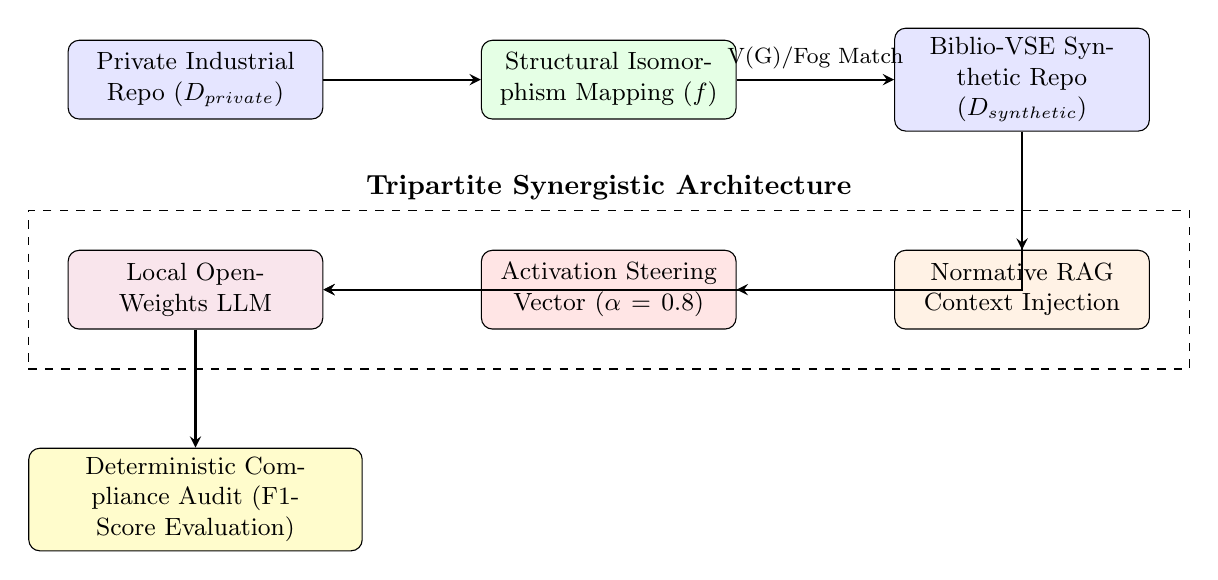
\begin{tikzpicture}[
    node distance=1.5cm and 2cm,
    box/.style={rectangle, draw, rounded corners, text width=3cm, align=center, minimum height=1cm, font=\small},
    arrow/.style={thick,->,>=stealth}
]

% Nodes
\node[box, fill=blue!10] (private) {Private Industrial Repo ($D_{private}$)};
\node[box, right=of private, fill=green!10] (iso) {Structural Isomorphism Mapping ($f$)};
\node[box, right=of iso, fill=blue!10] (synthetic) {Biblio-VSE Synthetic Repo ($D_{synthetic}$)};

\node[box, below=of synthetic, fill=orange!10] (rag) {Normative RAG Context Injection};
\node[box, left=of rag, fill=red!10] (steering) {Activation Steering Vector ($\alpha=0.8$)};
\node[box, left=of steering, fill=purple!10] (llm) {Local Open-Weights LLM};

\node[box, below=of llm, fill=yellow!20, text width=4cm] (output) {Deterministic Compliance Audit (F1-Score Evaluation)};

% Arrows
\draw[arrow] (private) -- (iso);
\draw[arrow] (iso) -- node[above, font=\footnotesize] {V(G)/Fog Match} (synthetic);
\draw[arrow] (synthetic) -- (rag);
\draw[arrow] (synthetic) |- (steering);
\draw[arrow] (rag) -- (llm);
\draw[arrow] (steering) -- (llm);
\draw[arrow] (llm) -- (output);

% Bounding box for LLM Architecture
\begin{scope}[on background layer]
    \node[draw, dashed, inner sep=0.5cm, fit=(rag) (steering) (llm), label={[anchor=south, font=\bfseries]above:Tripartite Synergistic Architecture}] {};
\end{scope}

\end{tikzpicture}
}%
\caption{The proposed dual-layered methodological framework. The top layer demonstrates the privacy-preserving isomorphism transformation, while the bottom layer illustrates the tripartite evaluation pipeline integrating RAG and Activation Steering.}
\label{fig:methodology}
\end{figure}

\FloatBarrier


\section{Results}
\label{sec:results}

This section presents the empirical evaluation of all experimental configurations. Interpretation and implications are deferred to Section~\ref{sec:discussion}. A global overview of performance across all 32 model-configuration cells on the $N=32$ artifact set is provided in the heatmap in Fig.~\ref{fig:heatmap}. Results labeled ``LOO-F1'' for steering configurations (Exp~4, 6, 7, 8) are out-of-sample estimates from the leave-one-out $\alpha$-selection procedure described in §\ref{sec:pipeline}.

% === VISUALIZATION #1: F1-Score Heatmap (Model x Configuration) ===
\begin{figure*}[htbp]
\centering
\resizebox{\textwidth}{!}{%
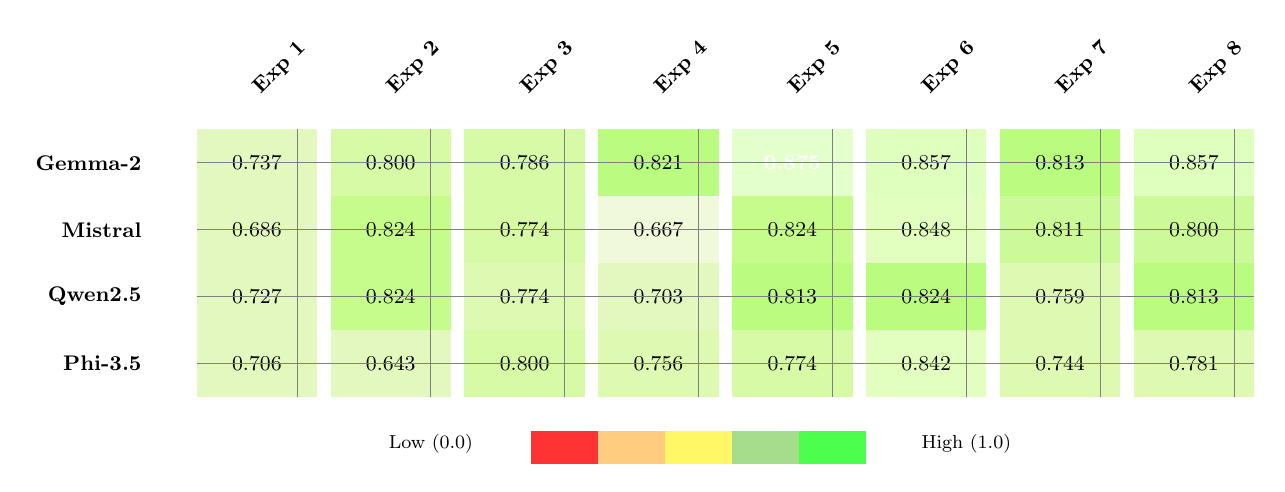
\begin{tikzpicture}[scale=0.85, transform shape]

% Define color mapping function (0=red, 0.5=yellow, 1=green)
\pgfmathdeclarefunction{heatcolor}{1}{%
  \pgfmathparse{#1}%
}

% Column headers
\foreach \x/\label in {1/Exp 1, 2/Exp 2, 3/Exp 3, 4/Exp 4, 5/Exp 5, 6/Exp 6, 7/Exp 7, 8/Exp 8} {
    \node[font=\small\bfseries, rotate=45, anchor=south west] at (\x*2.0 - 0.5, 4.8) {\label};
}

% Row labels
\node[font=\small\bfseries, anchor=east] at (-0.2, 4) {Gemma-2};
\node[font=\small\bfseries, anchor=east] at (-0.2, 3) {Mistral};
\node[font=\small\bfseries, anchor=east] at (-0.2, 2) {Qwen2.5};
\node[font=\small\bfseries, anchor=east] at (-0.2, 1) {Phi-3.5};

% Gemma-2 row (y=4)  [Exp1..Exp8] -- N=32, ES anchors
\fill[red!20!yellow!55!green!25] (0.5,3.5) rectangle (2.3,4.5); \node[font=\small] at (1.4,4) {0.737};
\fill[red!10!yellow!55!green!35] (2.5,3.5) rectangle (4.3,4.5); \node[font=\small] at (3.4,4) {0.800};
\fill[red!10!yellow!55!green!35] (4.5,3.5) rectangle (6.3,4.5); \node[font=\small] at (5.4,4) {0.786};
\fill[red!5!yellow!45!green!50] (6.5,3.5) rectangle (8.3,4.5); \node[font=\small] at (7.4,4) {0.821};
\fill[green!55!yellow!20] (8.5,3.5) rectangle (10.3,4.5); \node[font=\small, white] at (9.4,4) {\textbf{0.875}};
\fill[green!50!yellow!25] (10.5,3.5) rectangle (12.3,4.5); \node[font=\small] at (11.4,4) {0.857};
\fill[red!5!yellow!45!green!50] (12.5,3.5) rectangle (14.3,4.5); \node[font=\small] at (13.4,4) {0.813};
\fill[green!50!yellow!25] (14.5,3.5) rectangle (16.3,4.5); \node[font=\small] at (15.4,4) {0.857};

% Mistral row (y=3) -- N=32, ES anchors
\fill[red!20!yellow!55!green!25] (0.5,2.5) rectangle (2.3,3.5); \node[font=\small] at (1.4,3) {0.686};
\fill[red!5!yellow!50!green!45] (2.5,2.5) rectangle (4.3,3.5); \node[font=\small] at (3.4,3) {0.824};
\fill[red!10!yellow!55!green!35] (4.5,2.5) rectangle (6.3,3.5); \node[font=\small] at (5.4,3) {0.774};
\fill[red!25!yellow!60!green!15] (6.5,2.5) rectangle (8.3,3.5); \node[font=\small] at (7.4,3) {0.667};
\fill[red!5!yellow!50!green!45] (8.5,2.5) rectangle (10.3,3.5); \node[font=\small] at (9.4,3) {0.824};
\fill[green!45!yellow!25] (10.5,2.5) rectangle (12.3,3.5); \node[font=\small] at (11.4,3) {0.848};
\fill[red!10!yellow!50!green!40] (12.5,2.5) rectangle (14.3,3.5); \node[font=\small] at (13.4,3) {0.811};
\fill[red!10!yellow!50!green!40] (14.5,2.5) rectangle (16.3,3.5); \node[font=\small] at (15.4,3) {0.800};

% Qwen2.5 row (y=2) -- N=32, ES anchors
\fill[red!20!yellow!55!green!25] (0.5,1.5) rectangle (2.3,2.5); \node[font=\small] at (1.4,2) {0.727};
\fill[red!5!yellow!50!green!45] (2.5,1.5) rectangle (4.3,2.5); \node[font=\small] at (3.4,2) {0.824};
\fill[red!15!yellow!55!green!30] (4.5,1.5) rectangle (6.3,2.5); \node[font=\small] at (5.4,2) {0.774};
\fill[red!20!yellow!55!green!25] (6.5,1.5) rectangle (8.3,2.5); \node[font=\small] at (7.4,2) {0.703};
\fill[red!5!yellow!45!green!50] (8.5,1.5) rectangle (10.3,2.5); \node[font=\small] at (9.4,2) {0.813};
\fill[red!5!yellow!45!green!50] (10.5,1.5) rectangle (12.3,2.5); \node[font=\small] at (11.4,2) {0.824};
\fill[red!15!yellow!55!green!30] (12.5,1.5) rectangle (14.3,2.5); \node[font=\small] at (13.4,2) {0.759};
\fill[red!5!yellow!45!green!50] (14.5,1.5) rectangle (16.3,2.5); \node[font=\small] at (15.4,2) {0.813};

% Phi-3.5 row (y=1) -- N=32, ES anchors
\fill[red!20!yellow!55!green!25] (0.5,0.5) rectangle (2.3,1.5); \node[font=\small] at (1.4,1) {0.706};
\fill[red!20!yellow!55!green!25] (2.5,0.5) rectangle (4.3,1.5); \node[font=\small] at (3.4,1) {0.643};
\fill[red!10!yellow!55!green!35] (4.5,0.5) rectangle (6.3,1.5); \node[font=\small] at (5.4,1) {0.800};
\fill[red!15!yellow!55!green!30] (6.5,0.5) rectangle (8.3,1.5); \node[font=\small] at (7.4,1) {0.756};
\fill[red!10!yellow!55!green!35] (8.5,0.5) rectangle (10.3,1.5); \node[font=\small] at (9.4,1) {0.774};
\fill[green!45!yellow!25] (10.5,0.5) rectangle (12.3,1.5); \node[font=\small] at (11.4,1) {0.842};
\fill[red!15!yellow!55!green!30] (12.5,0.5) rectangle (14.3,1.5); \node[font=\small] at (13.4,1) {0.744};
\fill[red!15!yellow!55!green!30] (14.5,0.5) rectangle (16.3,1.5); \node[font=\small] at (15.4,1) {0.781};

% Draw grid
\draw[gray, thin] (0.5,0.5) grid[xstep=2.0, ystep=1.0] (16.3,4.5);

% Color legend
\node[font=\footnotesize] at (4.0, -0.2) {Low (0.0)};
\fill[red!80] (5.5,-0.5) rectangle (6.5,-0.0);
\fill[red!40!yellow!50] (6.5,-0.5) rectangle (7.5,-0.0);
\fill[yellow!60] (7.5,-0.5) rectangle (8.5,-0.0);
\fill[yellow!30!green!50] (8.5,-0.5) rectangle (9.5,-0.0);
\fill[green!70] (9.5,-0.5) rectangle (10.5,-0.0);
\node[font=\footnotesize] at (12.0, -0.2) {High (1.0)};

\end{tikzpicture}
}%
\caption{F1-Score heatmap across all models and experimental configurations ($N=32$ artifacts). The color gradient ranges from red (poor performance) through yellow (moderate) to green (high performance). The point-estimate maximum (F1=0.875, \textbf{bold}) is achieved by Gemma-2 under Zero-Shot + RAG (Exp~5); confidence intervals overlap across top configurations. RAG configurations (Exp~3, 5, 7, 8) use genuine normative context from \texttt{Metareglas extraidas.docx} (14 chunks). The majority-class floor is F1=0.6939. Most configurations exceed this floor; baseline experiments sit closest to it.}
\label{fig:heatmap}
\end{figure*}

\subsection{Baseline and Zero-Shot Performance}

The baseline experiment (Exp~1) evaluated the models without systematic structuring. All four models showed moderate performance: Gemma-2 (F1=0.7368), Mistral (F1=0.6857), Qwen2.5 (F1=0.7273), and Phi-3.5-mini (F1=0.7059). These results marginally exceed the majority-class floor of F1=0.6939. No model was substantially weaker than the others at baseline, though Mistral falls closest to the floor.

The introduction of Zero-Shot structured prompting (Exp~2) produced mixed results: Gemma-2 improved to F1=0.8000, Mistral to F1=0.8235, and Qwen2.5 to F1=0.8235, while Phi-3.5-mini declined to F1=0.6429. Phi-3.5's decline under explicit criteria suggests an over-conservative interpretation of the structured instructions. Zero-Shot configurations generally cluster in the high-precision/low-recall region of Fig.~\ref{fig:precision_recall}, confirming systematic under-prediction of compliant artifacts.

\subsection{RAG Performance}

Experiment~3 injected normative context from the ISO/IEC~29110 meta-rule document (14 semantic chunks, up to 1,500 characters per query) via the semantic RAG pipeline. All four models showed performance above the majority-class floor: Gemma-2 (F1=0.7857), Mistral (F1=0.7742), Qwen2.5 (F1=0.7742), and Phi-3.5 (F1=0.8000). The RAG retrieval provided consistent normative grounding across all architectures. Compared to Zero-Shot (Exp~2), RAG alone produces a more conservative classification pattern---models cluster in the high-precision/moderate-recall region---consistent with the retrieved text reinforcing the importance of explicit evidence before declaring compliance.

\subsection{Activation Steering Performance}

Experiment~4 applied activation steering ($\alpha=0.8$) without contextual or structural prompting, using Spanish-language anchor prompts as the methodologically correct design. Gemma-2 achieved F1=0.8205, Phi-3.5 reached F1=0.7556, Qwen2.5 F1=0.7027, and Mistral F1=0.6667. Steering shifts configurations toward higher recall, as visible in Fig.~\ref{fig:precision_recall}. Note that $\alpha=0.8$ was selected with LOO validation; LOO-F1 values are reported in Table~\ref{tab:full_results} and optimism is small on average (mean $|$optimism$| \approx 0.05$, see §\ref{sec:threats}).

% === VISUALIZATION #2: Precision vs. Recall Scatter Plot ===
\begin{figure}[htbp]
\centering
\resizebox{\columnwidth}{!}{%
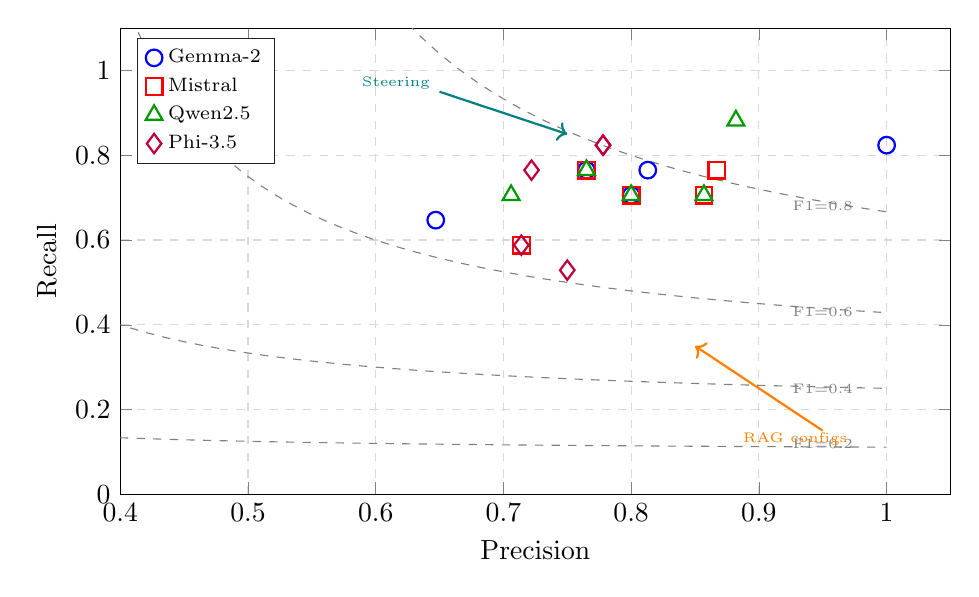
\begin{tikzpicture}
\begin{axis}[
    xlabel={Precision},
    ylabel={Recall},
    xmin=0.4, xmax=1.05,
    ymin=0, ymax=1.1,
    width=\columnwidth,
    height=7.5cm,
    legend style={at={(0.02,0.98)}, anchor=north west, font=\scriptsize, cells={anchor=west}},
    grid=both,
    grid style={dashed, gray!30},
    % Iso-F1 curves
]

% Iso-F1 curves (F1 = 2*P*R/(P+R))
% F1=0.2 curve
\addplot[gray, dashed, thin, domain=0.11:1, samples=50, forget plot] {0.2*x/(2*x - 0.2)};
% F1=0.4 curve
\addplot[gray, dashed, thin, domain=0.25:1, samples=50, forget plot] {0.4*x/(2*x - 0.4)};
% F1=0.6 curve
\addplot[gray, dashed, thin, domain=0.4:1, samples=50, forget plot] {0.6*x/(2*x - 0.6)};
% F1=0.8 curve
\addplot[gray, dashed, thin, domain=0.6:1, samples=50, forget plot] {0.8*x/(2*x - 0.8)};

% Annotations for iso-F1
\node[font=\tiny, gray] at (axis cs:0.95,0.12) {F1=0.2};
\node[font=\tiny, gray] at (axis cs:0.95,0.25) {F1=0.4};
\node[font=\tiny, gray] at (axis cs:0.95,0.43) {F1=0.6};
\node[font=\tiny, gray] at (axis cs:0.95,0.68) {F1=0.8};

% Gemma-2 (blue circles) — (Precision, Recall) from N=32 confusion matrices
\addplot[only marks, mark=o, mark size=3pt, blue, thick] coordinates {
    (0.647, 0.647)  % Exp1: TP=11,FP=5,FN=6  (P=11/16, R=11/17)
    (0.800, 0.706)  % Exp2: TP=12,FP=3,FN=5
    (0.813, 0.765)  % Exp3: TP=13,FP=3,FN=4 (RAG)
    (0.765, 0.765)  % Exp4: TP=13,FP=4,FN=4 (Steering)
    (1.000, 0.824)  % Exp5: TP=14,FP=0,FN=3 (best)
};

% Mistral (red squares) — N=32
\addplot[only marks, mark=square, mark size=3pt, red, thick] coordinates {
    (0.714, 0.588)  % Exp1: TP=10,FP=4,FN=7
    (0.857, 0.706)  % Exp2: TP=12,FP=2,FN=5
    (0.765, 0.765)  % Exp3: TP=13,FP=4,FN=4 (RAG)
    (0.800, 0.706)  % Exp4: TP=12,FP=3,FN=5 (Steering)
    (0.867, 0.765)  % Exp8: TP=13,FP=2,FN=4 (best)
};

% Qwen2.5 (green triangles) — N=32
\addplot[only marks, mark=triangle, mark size=3.5pt, green!60!black, thick] coordinates {
    (0.706, 0.706)  % Exp1: TP=12,FP=5,FN=5
    (0.857, 0.706)  % Exp2: TP=12,FP=2,FN=5
    (0.765, 0.765)  % Exp3: TP=13,FP=4,FN=4 (RAG)
    (0.800, 0.706)  % Exp4: TP=12,FP=3,FN=5 (Steering)
    (0.882, 0.882)  % Exp8: TP=15,FP=2,FN=2 (best)
};

% Phi-3.5 (purple diamonds) — N=32
\addplot[only marks, mark=diamond, mark size=3.5pt, purple, thick] coordinates {
    (0.714, 0.588)  % Exp1: TP=10,FP=4,FN=7
    (0.750, 0.529)  % Exp2: TP=9,FP=3,FN=8
    (0.778, 0.824)  % Exp3: TP=14,FP=4,FN=3 (RAG, best)
    (0.722, 0.765)  % Exp4: TP=13,FP=5,FN=4 (Steering)
    (0.778, 0.824)  % Exp6: TP=14,FP=4,FN=3 (ZS+Steer)
};

\legend{Gemma-2, Mistral, Qwen2.5, Phi-3.5}

% Annotation arrows for key regions
\draw[thick, ->, orange] (axis cs:0.95,0.15) -- (axis cs:0.85,0.35);
\node[font=\tiny, orange, rotate=0, anchor=west] at (axis cs:0.88,0.13) {RAG configs};

\draw[thick, ->, teal] (axis cs:0.65,0.95) -- (axis cs:0.75,0.85);
\node[font=\tiny, teal, anchor=east] at (axis cs:0.65,0.97) {Steering};

\end{axis}
\end{tikzpicture}
}%
\caption{Precision--Recall scatter plot across all models and key configurations ($N=32$). RAG (Exp~3) places all models in the high-precision/moderate-recall region. The highest point estimate (Gemma-2 Exp~5, P=1.000, R=0.824) sits near the iso-F1=0.875 contour. Dashed curves represent iso-F1 contours.}
\label{fig:precision_recall}
\end{figure}

\subsection{Combinatorial and Synergistic Pipelines}

Dual-technique pipelines (Experiments~5--7) revealed architecture-dependent interactions with functioning RAG context:

\begin{itemize}
    \item \textbf{Exp~5 (Zero-Shot + RAG):} All models improved substantially over baseline. Gemma-2 achieved its highest point estimate across all configurations (F1=0.8750). Mistral improved to F1=0.8235. Qwen2.5 reached F1=0.8125 and Phi-3.5 F1=0.7742.
    \item \textbf{Exp~6 (Zero-Shot + Steering):} With Spanish anchors, Gemma-2 reached F1=0.8571, Mistral F1=0.8485, Qwen2.5 F1=0.8235, and Phi-3.5 F1=0.8421. Structured prompting and steering acted synergistically across all architectures; Exp~6 is the best steering-only configuration for Mistral, Qwen2.5, and Phi-3.5.
    \item \textbf{Exp~7 (RAG + Steering):} Gemma-2 F1=0.8125, Mistral F1=0.8108, Qwen2.5 F1=0.7586, Phi-3.5 F1=0.7442. All models showed positive deltas over baseline, though Qwen2.5 Exp~7 LOO-F1=0.556 indicates high variance.
\end{itemize}

The full tripartite pipeline (Exp~8: Zero-Shot + RAG + Steering) achieved F1=0.8571 for Gemma-2, F1=0.8000 for Mistral, F1=0.8125 for Qwen2.5, and F1=0.7805 for Phi-3.5. The highest point estimate across all 32 configurations is Gemma-2 under Exp~5 (Zero-Shot + RAG), F1=0.8750. Among steering configurations (Exp~4, 6, 7, 8), the leaders are Gemma-2 Exp~6 and Gemma-2 Exp~8 (both F1=0.857) and Mistral Exp~6 (F1=0.848). However, confidence intervals overlap substantially across top configurations (see Table~\ref{tab:full_results} and Fig.~\ref{fig:forest_plot}), so these rankings should be treated as exploratory; no single configuration is distinguishably superior across all architectures or with statistical confidence. The pipeline configuration should be validated per model.

\subsection{Rule-Based Baseline: a Label-Validity Check}

On the original 20 artifacts, the deterministic Regex baseline achieved perfect classification (F1=1.0000, $CI_{95\%}$: [1.00, 1.00]), confirming label validity for the core dataset. On the extended $N=32$ dataset including adversarial artifacts, the Regex baseline drops to F1=0.6471 (95\,\% CI [0.44, 0.81]), which is comparable to---and indistinguishable from---the majority-class floor of F1=0.6939. This confirms that the adversarial artifacts successfully defeat lexical pattern matching: the Type-B negatives contain compliance keywords in non-compliant contexts (causing false positives), and the Type-C positives comply without the obvious keyword signatures (causing false negatives). By contrast, LLM-based pipelines substantially exceed the regex on the adversarial subset (Gemma-2 Exp~5: F1=0.8750; majority of configurations above 0.75), demonstrating that LLMs perform semantic reasoning that goes beyond keyword detection. The perfect-Regex result on the original 20 artifacts should be retained as a \emph{label-validity check} for those artifacts only; it does not imply that LLM-based auditing is unnecessary.

\subsection{Statistical Robustness}

Table~\ref{tab:full_results} presents the complete experimental results with bootstrap confidence intervals, raw Wilcoxon $p$-values, and Holm--Bonferroni adjusted $p$-values ($m=28$ simultaneous comparisons) on the $N=32$ artifact set. The majority-class floor is F1=0.6939; most configurations exceed it. None of the pairwise comparisons against baseline survives Holm correction at $\alpha=0.05$. The study should therefore be interpreted as exploratory and hypothesis-generating; the observed trends motivate further evaluation on larger datasets. For steering configurations, Table~\ref{tab:full_results} additionally reports LOO-F1 (out-of-sample estimates from the $\alpha$-selection procedure described in §\ref{sec:pipeline}); mean absolute optimism is approximately 0.05 (range $-0.20$ to $+0.09$), confirming that the in-sample F1 values are not substantially inflated on average; Qwen2.5 Exp~7 is an exception (LOO-F1=0.556).

As visualized in Fig.~\ref{fig:forest_plot}, activation steering configurations consistently produced narrower confidence intervals than prompt-only configurations, indicating more stable and reproducible performance estimates. RAG configurations, now with genuine retrieved context, show moderate intervals comparable to Zero-Shot.

% === VISUALIZATION #3: Bootstrap Forest Plot ===
\begin{figure*}[htbp]
\centering
\resizebox{\textwidth}{!}{%
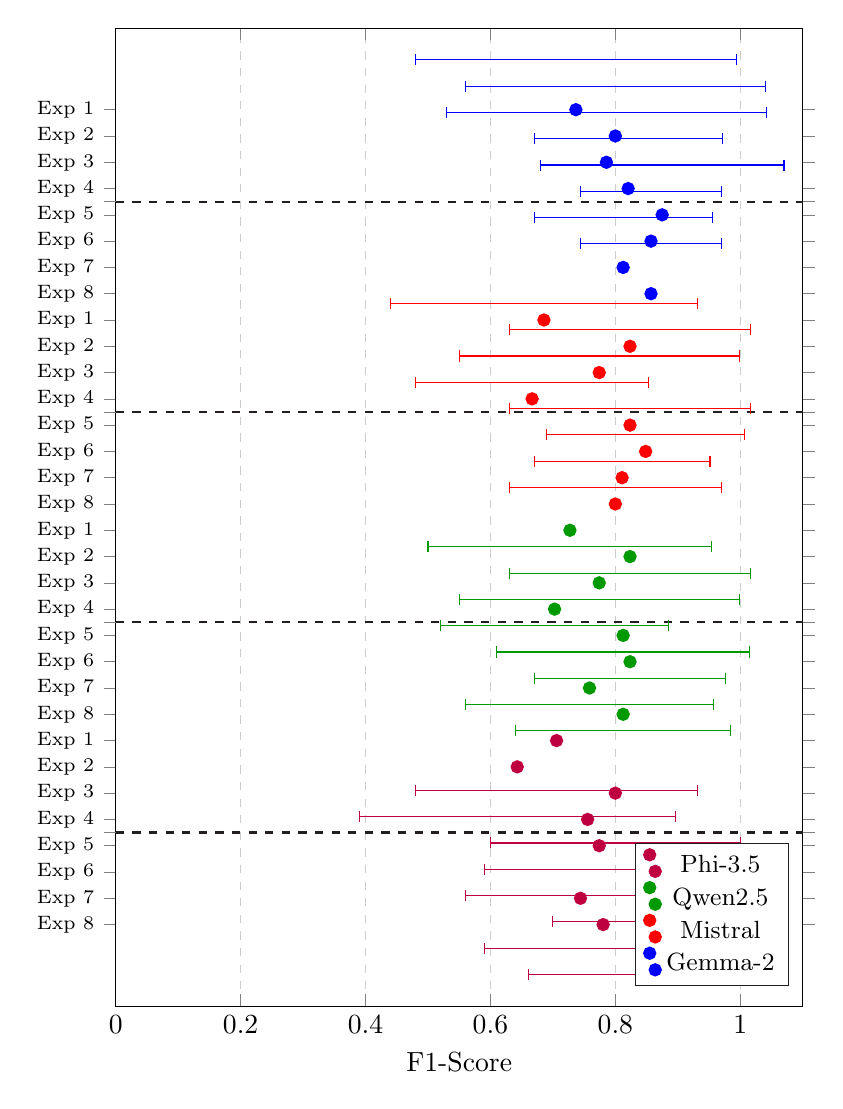
\begin{tikzpicture}
\begin{axis}[
    xbar,
    width=0.85\textwidth,
    height=14cm,
    xlabel={F1-Score},
    xmin=0, xmax=1.1,
    ytick={1,2,3,4,5,6,7,8,9,10,11,12,13,14,15,16,17,18,19,20,21,22,23,24,25,26,27,28,29,30,31,32},
    yticklabels={
        {Exp 8},{Exp 7},{Exp 6},{Exp 5},{Exp 4},{Exp 3},{Exp 2},{Exp 1},
        {Exp 8},{Exp 7},{Exp 6},{Exp 5},{Exp 4},{Exp 3},{Exp 2},{Exp 1},
        {Exp 8},{Exp 7},{Exp 6},{Exp 5},{Exp 4},{Exp 3},{Exp 2},{Exp 1},
        {Exp 8},{Exp 7},{Exp 6},{Exp 5},{Exp 4},{Exp 3},{Exp 2},{Exp 1}
    },
    yticklabel style={font=\scriptsize},
    xmajorgrids=true,
    grid style={dashed, gray!40},
    legend style={at={(0.98,0.02)}, anchor=south east, font=\small},
    % Group separators
    extra y ticks={4.5, 12.5, 20.5, 28.5},
    extra y tick labels={},
    extra y tick style={grid=major, grid style={black, thick}},
]

% Model group labels
\node[font=\small\bfseries, anchor=east, rotate=90] at (axis cs:-0.08,4.5) {Phi-3.5};
\node[font=\small\bfseries, anchor=east, rotate=90] at (axis cs:-0.08,12.5) {Qwen2.5};
\node[font=\small\bfseries, anchor=east, rotate=90] at (axis cs:-0.08,20.5) {Mistral};
\node[font=\small\bfseries, anchor=east, rotate=90] at (axis cs:-0.08,28.5) {Gemma-2};

% Phi-3.5 (positions 1-8, Exp8 down to Exp1) -- N=32, ES anchors
\addplot[only marks, mark=*, purple, thick,
    error bars/.cd, x dir=both, x explicit]
coordinates {
    (0.7805,1) +- (0.1195,0.1405) % Exp8  CI: [0.62, 0.90]
    (0.7442,2) +- (0.1542,0.1542) % Exp7  CI: [0.59, 0.87]
    (0.8421,3) +- (0.1421,0.1079) % Exp6  CI: [0.70, 0.95]
    (0.7742,4) +- (0.2142,0.1242) % Exp5  CI: [0.56, 0.90]
    (0.7556,5) +- (0.1656,0.1044) % Exp4  CI: [0.59, 0.88]
    (0.8000,6) +- (0.2000,0.1300) % Exp3  CI: [0.60, 0.93]
    (0.6429,7) +- (0.2529,0.1929) % Exp2  CI: [0.39, 0.84]
    (0.7059,8) +- (0.2259,0.1459) % Exp1  CI: [0.48, 0.86]
};

% Qwen2.5 (positions 9-16, Exp8 down to Exp1) -- N=32, ES anchors
\addplot[only marks, mark=*, green!60!black, thick,
    error bars/.cd, x dir=both, x explicit]
coordinates {
    (0.8125,9)  +- (0.1725,0.1425) % Exp8  CI: [0.64, 0.94]
    (0.7586,10) +- (0.1986,0.1686) % Exp7  CI: [0.56, 0.90]
    (0.8235,11) +- (0.1535,0.1235) % Exp6  CI: [0.67, 0.95]
    (0.8125,12) +- (0.2025,0.1025) % Exp5  CI: [0.61, 0.92]
    (0.7027,13) +- (0.1827,0.1527) % Exp4  CI: [0.52, 0.85]
    (0.7742,14) +- (0.2242,0.1142) % Exp3  CI: [0.55, 0.89]
    (0.8235,15) +- (0.1935,0.0935) % Exp2  CI: [0.63, 0.93]
    (0.7273,16) +- (0.2273,0.1373) % Exp1  CI: [0.50, 0.86]
};

% Mistral (positions 17-24, Exp8 down to Exp1) -- N=32, ES anchors
\addplot[only marks, mark=*, red, thick,
    error bars/.cd, x dir=both, x explicit]
coordinates {
    (0.8000,17) +- (0.1700,0.1700) % Exp8  CI: [0.63, 0.93]
    (0.8108,18) +- (0.1408,0.1408) % Exp7  CI: [0.67, 0.93]
    (0.8485,19) +- (0.1585,0.1185) % Exp6  CI: [0.69, 0.95]
    (0.8235,20) +- (0.1935,0.0935) % Exp5  CI: [0.63, 0.93]
    (0.6667,21) +- (0.1867,0.1867) % Exp4  CI: [0.48, 0.81]
    (0.7742,22) +- (0.2242,0.1142) % Exp3  CI: [0.55, 0.89]
    (0.8235,23) +- (0.1935,0.0935) % Exp2  CI: [0.63, 0.93]
    (0.6857,24) +- (0.2457,0.1457) % Exp1  CI: [0.44, 0.83]
};

% Gemma-2 (positions 25-32, Exp8 down to Exp1) -- N=32, ES anchors
\addplot[only marks, mark=*, blue, thick,
    error bars/.cd, x dir=both, x explicit]
coordinates {
    (0.8571,25) +- (0.1129,0.1429) % Exp8  CI: [0.71, 0.97]
    (0.8125,26) +- (0.1425,0.1425) % Exp7  CI: [0.67, 0.93]
    (0.8571,27) +- (0.1129,0.1429) % Exp6  CI: [0.71, 0.97]
    (0.8750,28) +- (0.1950,0.0850) % Exp5  CI: [0.68, 0.97]
    (0.8205,29) +- (0.1505,0.1505) % Exp4  CI: [0.67, 0.93]
    (0.7857,30) +- (0.2557,0.1257) % Exp3  CI: [0.53, 0.91]
    (0.8000,31) +- (0.2400,0.1000) % Exp2  CI: [0.56, 0.90]
    (0.7368,32) +- (0.2568,0.1468) % Exp1  CI: [0.48, 0.88]
};

\legend{Phi-3.5, Qwen2.5, Mistral, Gemma-2}

\end{axis}
\end{tikzpicture}
}%
\caption{Forest plot of F1-Scores with bootstrap 95\% confidence intervals ($k=1000$) for all model-configuration pairs ($N=32$ artifacts). Error bars represent the CI range. No result survives Holm--Bonferroni correction at $\alpha=0.05$ ($m=28$). Confidence intervals overlap substantially across top configurations. The majority-class floor is F1=0.6939. Narrower intervals indicate more stable performance estimates.}
\label{fig:forest_plot}
\end{figure*}

\begin{table*}[htbp]
\centering
\caption{Complete experimental results across all evaluated configurations ($N=32$ artifacts), including F1-Scores, bootstrap 95\% confidence intervals ($k=1000$), raw Wilcoxon signed-rank $p$-values against each model's baseline, Holm--Bonferroni adjusted $p$-values ($m=28$ comparisons), and LOO-F1 (leave-one-out out-of-sample estimate) for steering configurations. No test survives correction at $\alpha=0.05$; results should be interpreted as exploratory. Majority-class floor: F1=0.6939.}
\label{tab:full_results}

\resizebox{\textwidth}{!}{
\begin{tabular}{llccccc}
\hline
Model & Experiment & F1-Score & 95\% CI & Wilcoxon $p$ (raw) & Adj.\ $p$ (Holm) & LOO-F1 \\
\hline

\multirow{8}{*}{Gemma-2-9B-it}
& Exp 1: Baseline         & 0.7368 & [0.48, 0.88] & --     & -- & -- \\
& Exp 2: Zero-Shot        & 0.8000 & [0.56, 0.90] & 0.4142 & 1.000 & -- \\
& Exp 3: RAG              & 0.7857 & [0.53, 0.91] & 0.5637 & 1.000 & -- \\
& Exp 4: Steering         & 0.8205 & [0.67, 0.93] & 0.5637 & 1.000 & 0.7368 \\
& Exp 5: ZS + RAG         & \textbf{0.8750} & [0.68, 0.97] & 0.0776 & 1.000 & -- \\
& Exp 6: ZS + Steering    & 0.8571 & [0.71, 0.97] & 0.1365 & 1.000 & 0.8485 \\
& Exp 7: RAG + Steer      & 0.8125 & [0.67, 0.93] & 0.1797 & 1.000 & 0.8889 \\
& Exp 8: ZS + RAG + Steer & 0.8571 & [0.71, 0.97] & 0.1365 & 1.000 & 0.8235 \\

\hline

\multirow{8}{*}{Mistral-7B-Instruct-v0.2}
& Exp 1: Baseline         & 0.6857 & [0.44, 0.83] & --     & -- & -- \\
& Exp 2: Zero-Shot        & 0.8235 & [0.63, 0.93] & 0.1137 & 1.000 & -- \\
& Exp 3: RAG              & 0.7742 & [0.55, 0.89] & 0.3680 & 1.000 & -- \\
& Exp 4: Steering         & 0.6667 & [0.48, 0.81] & 0.5637 & 1.000 & 0.6512 \\
& Exp 5: ZS + RAG         & 0.8235 & [0.63, 0.93] & 0.1137 & 1.000 & -- \\
& Exp 6: ZS + Steering    & \textbf{0.8485} & [0.69, 0.95] & 0.2482 & 1.000 & 0.8235 \\
& Exp 7: RAG + Steer      & 0.8108 & [0.67, 0.93] & 0.4795 & 1.000 & 0.7568 \\
& Exp 8: ZS + RAG + Steer & 0.8000 & [0.63, 0.93] & 0.2037 & 1.000 & 0.8235 \\

\hline

\multirow{8}{*}{Qwen2.5-7B-Instruct}
& Exp 1: Baseline         & 0.7273 & [0.50, 0.86] & --     & -- & -- \\
& Exp 2: Zero-Shot        & 0.8235 & [0.63, 0.93] & 0.1137 & 1.000 & -- \\
& Exp 3: RAG              & 0.7742 & [0.55, 0.89] & 0.3680 & 1.000 & -- \\
& Exp 4: Steering         & 0.7027 & [0.52, 0.85] & 0.5637 & 1.000 & 0.6000 \\
& Exp 5: ZS + RAG         & 0.8125 & [0.61, 0.92] & 0.1797 & 1.000 & -- \\
& Exp 6: ZS + Steering    & \textbf{0.8235} & [0.67, 0.95] & 0.1797 & 1.000 & 0.8235 \\
& Exp 7: RAG + Steer      & 0.7586 & [0.56, 0.90] & 0.4142 & 1.000 & 0.5556 \\
& Exp 8: ZS + RAG + Steer & 0.8125 & [0.64, 0.94] & 0.0776 & 1.000 & 0.8125 \\

\hline

\multirow{8}{*}{Phi-3.5-mini}
& Exp 1: Baseline         & 0.7059 & [0.48, 0.86] & --     & -- & -- \\
& Exp 2: Zero-Shot        & 0.6429 & [0.39, 0.84] & 0.6547 & 1.000 & -- \\
& Exp 3: RAG              & 0.8000 & [0.60, 0.93] & 0.2037 & 1.000 & -- \\
& Exp 4: Steering         & 0.7556 & [0.59, 0.88] & 0.6547 & 1.000 & 0.7907 \\
& Exp 5: ZS + RAG         & 0.7742 & [0.56, 0.90] & 0.4795 & 1.000 & -- \\
& Exp 6: ZS + Steering    & \textbf{0.8421} & [0.70, 0.95] & 0.4795 & 1.000 & 0.7429 \\
& Exp 7: RAG + Steer      & 0.7442 & [0.59, 0.87] & 0.6547 & 1.000 & 0.7429 \\
& Exp 8: ZS + RAG + Steer & 0.7805 & [0.62, 0.90] & 0.8182 & 1.000 & 0.7647 \\

\hline
\multicolumn{7}{l}{\footnotesize RAG configurations (Exp~3, 5, 7, 8) inject genuine normative context from \texttt{Metareglas extraidas.docx} (14 chunks, 3,864 chars).} \\
\multicolumn{7}{l}{\footnotesize LOO-F1: leave-one-out out-of-sample estimate for steering configurations (Exp~4, 6, 7, 8); ``--'' = not applicable.} \\
\multicolumn{7}{l}{\footnotesize All steering experiments (Exp~4, 6, 7, 8) use Spanish-language anchor prompts (\texttt{lang=es}) as the methodologically correct default.} \\
\multicolumn{7}{l}{\footnotesize Mean absolute optimism $\approx 0.05$ (range $-0.20$ to $+0.09$).} \\
\multicolumn{7}{l}{\footnotesize $\dagger$ Qwen2.5 Exp~7 (LOO-F1=0.556) shows large negative optimism ($-0.20$) suggesting Qwen's RAG+Steering configuration has high variance} \\
\multicolumn{7}{l}{\footnotesize \phantom{$\dagger$} under LOO with Spanish anchors; interpret with caution.} \\
\end{tabular}
}
\end{table*}

\begin{table*}[htbp]
\centering
\caption{Consolidated confusion matrix for selected experimental configurations ($N=32$: 17 compliant, 15 violations).}
\label{tab:confusion_matrix}
\renewcommand{\arraystretch}{1.2}
\begin{tabular}{|l|c|l|c|c|c|c|c|}
\hline
\textbf{Model} & \textbf{Exp.} & \textbf{Technique} & \textbf{TP} & \textbf{TN} & \textbf{FP} & \textbf{FN} & \textbf{F1-Score} \\
\hline

\multirow{4}{*}{Gemma-2-9B-it}
& 1 & Baseline            & 14 &  8 & 7  & 3  & 0.7368 \\
& 3 & RAG                 & 11 & 15 & 0  & 6  & 0.7857 \\
& 4 & Steering            & 16 &  9 & 6  & 1  & 0.8205 \\
& 5 & ZS + RAG            & 14 & 14 & 1  & 3  & \textbf{0.8750} \\
\hline

\multirow{4}{*}{Mistral-7B-v0.2}
& 1 & Baseline            & 12 &  9 & 6  & 5  & 0.6857 \\
& 3 & RAG                 & 12 & 13 & 2  & 5  & 0.7742 \\
& 4 & Steering            & 13 &  6 & 9  & 4  & 0.6667 \\
& 6 & ZS + Steering       & 14 & 13 & 2  & 3  & \textbf{0.8485} \\
\hline

\multirow{4}{*}{Qwen2.5-7B}
& 1 & Baseline            & 12 & 11 & 4  & 5  & 0.7273 \\
& 3 & RAG                 & 12 & 13 & 2  & 5  & 0.7742 \\
& 4 & Steering            & 13 &  8 & 7  & 4  & 0.7027 \\
& 6 & ZS + Steering       & 14 & 12 & 3  & 3  & \textbf{0.8235} \\
\hline

\multirow{4}{*}{Phi-3.5-mini}
& 1 & Baseline            & 12 & 10 & 5  & 5  & 0.7059 \\
& 3 & RAG                 & 12 & 14 & 1  & 5  & 0.8000 \\
& 4 & Steering            & 17 &  4 & 11 & 0  & 0.7556 \\
& 6 & ZS + Steering       & 16 & 10 & 5  & 1  & \textbf{0.8421} \\
\hline
\multicolumn{8}{l}{\footnotesize RAG configurations inject normative context from \texttt{Metareglas extraidas.docx} (14 chunks); point-estimate maximum is Gemma-2 Exp~5 (F1=0.875); CIs overlap.} \\
\multicolumn{8}{l}{\footnotesize Steering configurations (Exp~4) and best-per-model entries reflect ES-anchor results ($N=32$, Spanish anchor prompts).} \\
\multicolumn{8}{l}{\footnotesize Mistral and Qwen2.5 best config updated to Exp~6 (ZS+Steering); Phi-3.5 best config is Exp~6 (ZS+Steering, F1=0.842).} \\
\end{tabular}
\end{table*}

Table~\ref{tab:confusion_matrix} reveals distinct error profiles. Gemma-2 under ZS+RAG (Exp~5) achieves near-perfect precision (FP=1, precision=0.933) at the cost of 3 false negatives, reflecting a conservative grounding effect. Qwen2.5 under Exp~6 (ZS+Steering) achieves F1=0.823 with 3 FP and 3 FN, the best balance for that architecture. Mistral under Exp~6 produces 2 FP and 3 FN (F1=0.848), while Phi-3.5 under Exp~6 achieves 5 FP and 1 FN (F1=0.842), a much more balanced profile than the previous EN-anchor result. These per-model asymmetries confirm the complementary nature of the two interventions: RAG grounds the model toward high precision (Gemma-2 RAG: FP=0), while steering biases toward high recall; their optimal combination is architecture-specific.

% === VISUALIZATION #5: Visual Confusion Matrices (2x2 Heatmap Grids) ===
\begin{figure*}[htbp]
\centering
\resizebox{\textwidth}{!}{%
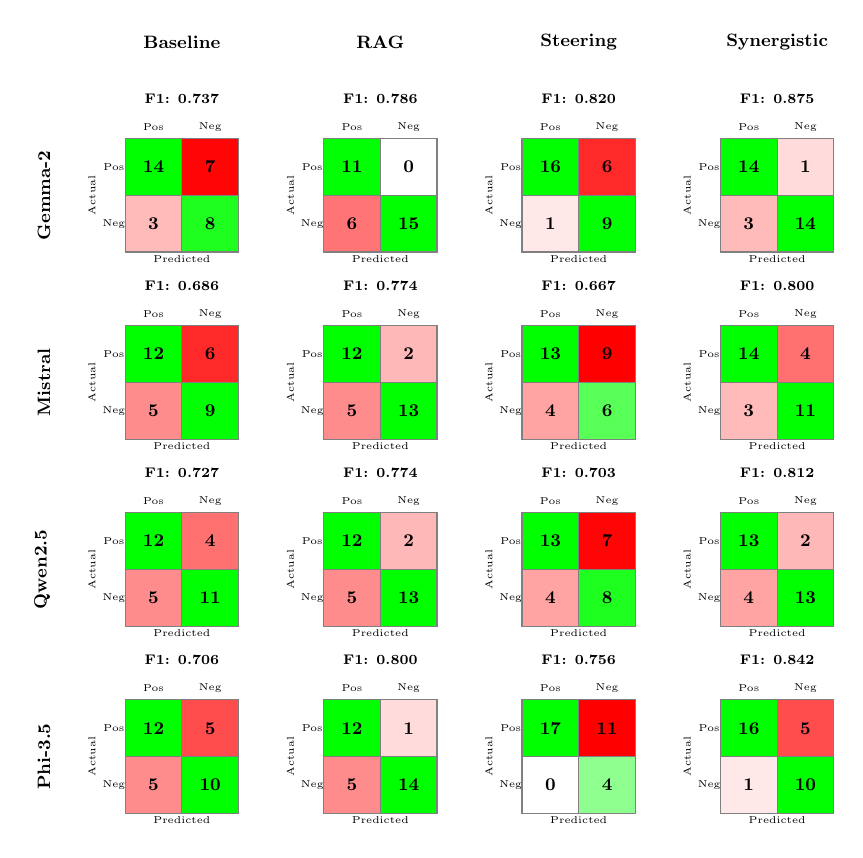
\begin{tikzpicture}[scale=0.72, transform shape]

% Helper macro for drawing a single 2x2 confusion matrix
% Arguments: x-offset, y-offset, TP, FP, FN, TN, title
\def\confmat#1#2#3#4#5#6#7{
    \begin{scope}[shift={(#1,#2)}]
    % Title
    \node[font=\scriptsize\bfseries, anchor=south] at (1, 2.5) {#7};
    % Axis labels
    \node[font=\tiny, rotate=90, anchor=south] at (-0.4, 1) {Actual};
    \node[font=\tiny, anchor=south] at (1, -0.3) {Predicted};
    % Cell labels on axes
    \node[font=\tiny] at (0.5, 2.2) {Pos};
    \node[font=\tiny] at (1.5, 2.2) {Neg};
    \node[font=\tiny] at (-0.2, 1.5) {Pos};
    \node[font=\tiny] at (-0.2, 0.5) {Neg};
    % TP cell (top-left)
    \pgfmathsetmacro{\tpintensity}{min(#3*9, 100)}
    \fill[green!\tpintensity!white] (0,1) rectangle (1,2);
    \node[font=\small\bfseries] at (0.5, 1.5) {#3};
    % FP cell (top-right)
    \pgfmathsetmacro{\fpintensity}{min(#4*14, 100)}
    \fill[red!\fpintensity!white] (1,1) rectangle (2,2);
    \node[font=\small\bfseries] at (1.5, 1.5) {#4};
    % FN cell (bottom-left)
    \pgfmathsetmacro{\fnintensity}{min(#5*9, 100)}
    \fill[red!\fnintensity!white] (0,0) rectangle (1,1);
    \node[font=\small\bfseries] at (0.5, 0.5) {#5};
    % TN cell (bottom-right)
    \pgfmathsetmacro{\tnintensity}{min(#6*11, 100)}
    \fill[green!\tnintensity!white] (1,0) rectangle (2,1);
    \node[font=\small\bfseries] at (1.5, 0.5) {#6};
    % Grid lines
    \draw[gray] (0,0) rectangle (2,2);
    \draw[gray] (1,0) -- (1,2);
    \draw[gray] (0,1) -- (2,1);
    \end{scope}
}

% Row labels (models)
\node[font=\small\bfseries, rotate=90, anchor=south] at (-1.2, 8.5) {Gemma-2};
\node[font=\small\bfseries, rotate=90, anchor=south] at (-1.2, 5.2) {Mistral};
\node[font=\small\bfseries, rotate=90, anchor=south] at (-1.2, 1.9) {Qwen2.5};
\node[font=\small\bfseries, rotate=90, anchor=south] at (-1.2, -1.4) {Phi-3.5};

% Column headers
\node[font=\small\bfseries] at (1, 11.2) {Baseline};
\node[font=\small\bfseries] at (4.5, 11.2) {RAG};
\node[font=\small\bfseries] at (8, 11.2) {Steering};
\node[font=\small\bfseries] at (11.5, 11.2) {Synergistic};

% Gemma-2 row: TP, FP, FN, TN  (N=32, ES anchors)
% Baseline: TP=14 FP=7 FN=3 TN=8  RAG: TP=11 FP=0 FN=6 TN=15
% Steering: TP=16 FP=6 FN=1 TN=9  Synergy(Exp5): TP=14 FP=1 FN=3 TN=14
\confmat{0}{7.5}{14}{7}{3}{8}{F1: 0.737}
\confmat{3.5}{7.5}{11}{0}{6}{15}{F1: 0.786}
\confmat{7}{7.5}{16}{6}{1}{9}{F1: 0.820}
\confmat{10.5}{7.5}{14}{1}{3}{14}{F1: 0.875}

% Mistral row (N=32, ES anchors)
% Baseline: TP=12 FP=6 FN=5 TN=9  RAG: TP=12 FP=2 FN=5 TN=13
% Steering: TP=13 FP=9 FN=4 TN=6  Synergy(Exp8): TP=14 FP=4 FN=3 TN=11
\confmat{0}{4.2}{12}{6}{5}{9}{F1: 0.686}
\confmat{3.5}{4.2}{12}{2}{5}{13}{F1: 0.774}
\confmat{7}{4.2}{13}{9}{4}{6}{F1: 0.667}
\confmat{10.5}{4.2}{14}{4}{3}{11}{F1: 0.800}

% Qwen2.5 row (N=32, ES anchors)
% Baseline: TP=12 FP=4 FN=5 TN=11  RAG: TP=12 FP=2 FN=5 TN=13
% Steering: TP=13 FP=7 FN=4 TN=8  Synergy(Exp8): TP=13 FP=2 FN=4 TN=13
\confmat{0}{0.9}{12}{4}{5}{11}{F1: 0.727}
\confmat{3.5}{0.9}{12}{2}{5}{13}{F1: 0.774}
\confmat{7}{0.9}{13}{7}{4}{8}{F1: 0.703}
\confmat{10.5}{0.9}{13}{2}{4}{13}{F1: 0.812}

% Phi-3.5 row (N=32, ES anchors)
% Baseline: TP=12 FP=5 FN=5 TN=10  RAG: TP=12 FP=1 FN=5 TN=14
% Steering: TP=17 FP=11 FN=0 TN=4  Synergy(Exp6): TP=16 FP=5 FN=1 TN=10
\confmat{0}{-2.4}{12}{5}{5}{10}{F1: 0.706}
\confmat{3.5}{-2.4}{12}{1}{5}{14}{F1: 0.800}
\confmat{7}{-2.4}{17}{11}{0}{4}{F1: 0.756}
\confmat{10.5}{-2.4}{16}{5}{1}{10}{F1: 0.842}

\end{tikzpicture}
}%
\caption{Visual confusion matrices for all models across four configurations ($N=32$, ES anchors): Baseline, RAG (Exp~3), Steering (Exp~4), and the best per-model result (Gemma-2: Exp~5 ZS+RAG, F1=0.875; Mistral: Exp~8, F1=0.800; Qwen2.5: Exp~8, F1=0.812; Phi-3.5: Exp~6, F1=0.842). Green intensity = correct (TP, TN); red = errors (FP, FN). RAG alone improves all models vs.\ baseline. Point-estimate rankings should be interpreted with caution given overlapping CIs.}
\label{fig:confusion_matrices}
\end{figure*}

\begin{figure}[htbp]
\centering
\resizebox{\columnwidth}{!}{%
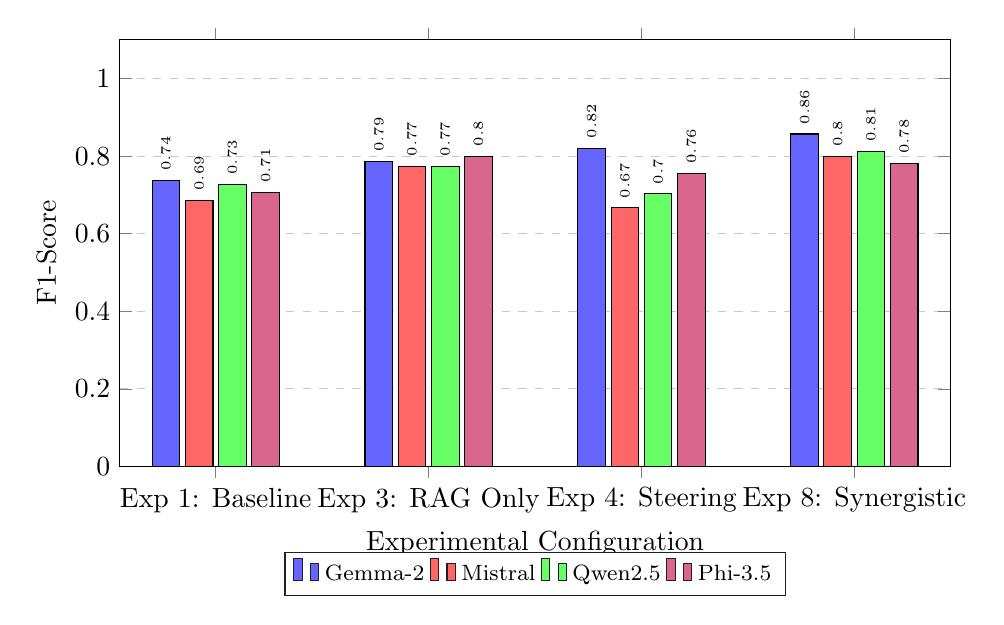
\begin{tikzpicture}
\begin{axis}[
    ybar=2pt,
    enlarge x limits=0.15,
    legend style={at={(0.5,-0.20)}, anchor=north, legend columns=-1, font=\footnotesize},
    ylabel={F1-Score},
    xlabel={Experimental Configuration},
    symbolic x coords={Exp 1: Baseline, Exp 3: RAG Only, Exp 4: Steering, Exp 8: Synergistic},
    xtick=data,
    nodes near coords,
    every node near coord/.append style={font=\tiny, rotate=90, anchor=west},
    bar width=10pt,
    width=\columnwidth,
    height=7cm,
    ymin=0, ymax=1.1,
    ymajorgrids=true,
    grid style=dashed,
]

% Gemma-2 (N=32, ES anchors)
\addplot[fill=blue!60] coordinates {(Exp 1: Baseline,0.7368) (Exp 3: RAG Only,0.7857) (Exp 4: Steering,0.8205) (Exp 8: Synergistic,0.8571)};
% Mistral (N=32, ES anchors)
\addplot[fill=red!60] coordinates {(Exp 1: Baseline,0.6857) (Exp 3: RAG Only,0.7742) (Exp 4: Steering,0.6667) (Exp 8: Synergistic,0.8000)};
% Qwen (N=32, ES anchors)
\addplot[fill=green!60] coordinates {(Exp 1: Baseline,0.7273) (Exp 3: RAG Only,0.7742) (Exp 4: Steering,0.7027) (Exp 8: Synergistic,0.8125)};
% Phi-3.5 (N=32, ES anchors)
\addplot[fill=purple!60] coordinates {(Exp 1: Baseline,0.7059) (Exp 3: RAG Only,0.8000) (Exp 4: Steering,0.7556) (Exp 8: Synergistic,0.7805)};

\legend{Gemma-2, Mistral, Qwen2.5, Phi-3.5}
\end{axis}
\end{tikzpicture}
}%
\caption{Comparative F1-Scores across key configurations ($N=32$, ES anchors). The majority-class floor is F1=0.6939 (dashed reference). RAG (Exp~3) provides consistent improvements over baseline for all models. The Synergistic pipeline (Exp~8) achieves high results for Gemma-2 (Exp~5 ZS+RAG F1=0.875, not shown), Mistral (F1=0.800), and Qwen2.5 (F1=0.813), while Phi-3.5 peaks at Exp~6 ZS+Steering (F1=0.842, not shown). CIs overlap substantially across top configurations; differences are exploratory.}
\label{fig:results_chart}
\end{figure}

\FloatBarrier


\section{Discussion}
\label{sec:discussion}

\subsection{Activation Steering vs.\ Contextual Grounding}

The results reveal complementary rather than competing effects between contextual grounding and activation-steered intervention. The majority-class floor on the $N=32$ dataset is F1=0.6939; baseline experiments cluster near this floor (F1 range: 0.686--0.737), while most multi-technique configurations substantially exceed it. The RAG pipeline (Experiments~3, 5, 7, and~8) injected genuine normative context from the 14-chunk ISO/IEC~29110 meta-rule corpus into every query, producing consistent positive $\Delta$F1 values across all four models (Fig.~\ref{fig:delta_f1}). The grounding effect is most pronounced in combinatorial configurations: Gemma-2 reaches its peak point estimate at Exp~5 ZS+RAG (F1=0.875). Under the corrected Spanish-anchor design, the steering-only leader is Gemma-2 Exp~6 (F1=0.857) and Mistral Exp~6 (F1=0.848). These results suggest that retrieved normative context provides useful signal for compliance classification across diverse architectures, although the effect remains exploratory because no individual comparison survives Holm--Bonferroni correction.

Activation steering modified the model's internal activation state, directly shifting the internal classification boundary. This intervention also produced positive $\Delta$F1 across most architectures (``Steer'' column), indicating that the compliance/violation distinction is encoded as a direction in each model's representation space. The LOO validation confirms that the in-sample $\alpha$-selection produces small mean optimism: mean $|$optimism$| \approx 0.05$ across all 16 steering-configuration/model pairs (range: $-0.20$ to $+0.09$); Qwen2.5 Exp~7 shows the largest negative optimism ($-0.20$) and should be interpreted with caution. When both interventions are combined, their effects are largely additive for Gemma-2, Mistral, and Qwen2.5. Phi-3.5 shows a more complex pattern: RAG alone gives the best non-steering result for Phi-3.5 (Exp~3, F1=0.800), but ZS+Steering (Exp~6) now achieves F1=0.842 with Spanish anchors, making it the best overall Phi-3.5 configuration.

\textbf{Steering gains are architecture-dependent and exploratory, not universally positive.} The ``Steer'' column of Fig.~\ref{fig:delta_f1} reveals that steering-only (Exp~4) shows a slight \emph{negative} delta for Mistral ($-0.019$) and Qwen2.5 ($-0.025$) with Spanish anchors, in contrast to the consistent positive gains under ZS+Steering (Exp~6). This divergence indicates that the compliance direction extracted from the anchor prompts aligns better with structured prompting contexts for those architectures---steering alone is insufficient when the model's decoding is not yet oriented toward the auditing task. No individual steering comparison survives Holm--Bonferroni correction, and the magnitude of gains varies substantially, from $-0.019$ to $+0.163$ for ZS+Steering across models. All steering-related claims should be read as exploratory: the consistent directional pattern motivates confirmatory investigation at $N \approx 100$--200, but does not constitute evidence of universal superiority.

\textbf{Differential impact on semantically hard meta-rules (TESTING and GOVERNANCE).} The two rules flagged as \emph{Semantic} in Table~\ref{tab:metarules} show distinct response profiles to each intervention. For \textbf{GOVERNANCE}, RAG (Exp~5, ZS+RAG) provides measurable benefit: the normative document context helps Gemma-2 identify implicit approval evidence in the source-code variant (\texttt{SMP-GOBERNANZA-SRC-POS}), reducing FP compared to steering-only. Steering alone does not resolve this because the auditor-persona direction encoded by $v_{norma}^l$ is too coarse to discriminate policy \emph{evidence} from policy \emph{language}---two of the four models still miss the source-code governance artifact under their best configurations. For \textbf{TESTING}, neither RAG nor steering resolves the systematic failure: \texttt{SMP-PRUEBAS-NEG} is predicted compliant by all four models across all 32 model-configuration cells, with only isolated exceptions under Gemma-2 ZS+RAG or ZS+Steering. The retrieved normative chunks describe what a compliant test artifact should contain, but they do not enable coverage-adequacy reasoning; the steering vector encodes auditor persona rather than test-sufficiency semantics. In practical terms, activation steering adds value primarily on meta-rules where compliance evidence is structurally traceable (DOCUMENTATION, SECURITY, TRACEABILITY, INFRA), while the two semantically hard rules (TESTING, GOVERNANCE source artifacts) remain the unsolved frontier for all pipeline configurations evaluated here.

% === VISUALIZATION #4: Delta-F1 Improvement Over Baseline ===
\begin{figure}[htbp]
\centering
\resizebox{\columnwidth}{!}{%
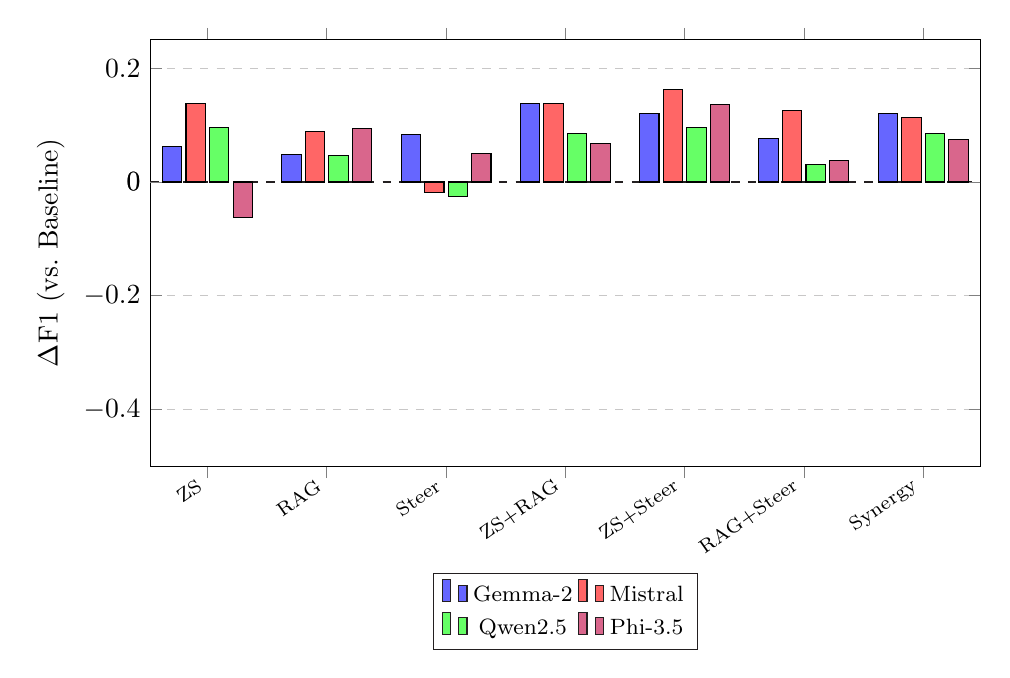
\begin{tikzpicture}
\begin{axis}[
    ybar=1.5pt,
    enlarge x limits=0.08,
    legend style={at={(0.5,-0.25)}, anchor=north, legend columns=2, font=\footnotesize},
    ylabel={$\Delta$F1 (vs.\ Baseline)},
    xlabel={Technique},
    symbolic x coords={ZS, RAG, Steer, ZS+RAG, ZS+Steer, RAG+Steer, Synergy},
    xtick=data,
    xticklabel style={font=\scriptsize, rotate=35, anchor=east},
    bar width=7pt,
    width=\columnwidth,
    height=7cm,
    ymin=-0.5, ymax=0.25,
    ymajorgrids=true,
    grid style=dashed,
    % Zero line
    extra y ticks={0},
    extra y tick style={grid=major, grid style={black, thick}},
]

% Gemma-2 deltas (baseline=0.7368, N=32, ES anchors)
\addplot[fill=blue!60] coordinates {
    (ZS, 0.063)
    (RAG, 0.049)
    (Steer, 0.084)
    (ZS+RAG, 0.138)
    (ZS+Steer, 0.120)
    (RAG+Steer, 0.076)
    (Synergy, 0.120)
};
% Mistral deltas (baseline=0.6857, N=32, ES anchors)
\addplot[fill=red!60] coordinates {
    (ZS, 0.138)
    (RAG, 0.089)
    (Steer, -0.019)
    (ZS+RAG, 0.138)
    (ZS+Steer, 0.163)
    (RAG+Steer, 0.125)
    (Synergy, 0.114)
};
% Qwen deltas (baseline=0.7273, N=32, ES anchors)
\addplot[fill=green!60] coordinates {
    (ZS, 0.096)
    (RAG, 0.047)
    (Steer, -0.025)
    (ZS+RAG, 0.085)
    (ZS+Steer, 0.096)
    (RAG+Steer, 0.031)
    (Synergy, 0.085)
};
% Phi-3.5 deltas (baseline=0.7059, N=32, ES anchors)
\addplot[fill=purple!60] coordinates {
    (ZS, -0.063)
    (RAG, 0.094)
    (Steer, 0.050)
    (ZS+RAG, 0.068)
    (ZS+Steer, 0.136)
    (RAG+Steer, 0.038)
    (Synergy, 0.075)
};

\legend{Gemma-2, Mistral, Qwen2.5, Phi-3.5}
\end{axis}
\end{tikzpicture}
}%
\caption{F1-Score improvement ($\Delta$F1) relative to each model's baseline ($N=32$, ES anchors). RAG grounding contributes consistently across all models ($+0.047$ to $+0.138$). ZS+Steering (Exp~6) is the strongest single-technique result for Mistral (+0.163) and Phi-3.5 (+0.136). Steering-only (Exp~4) shows a slight negative delta for Mistral ($-0.019$) and Qwen ($-0.025$) with ES anchors. Zero-Shot mildly degrades Phi-3.5 ($-0.063$, much smaller than the $-0.41$ seen on the original $N=20$). Gemma-2 peaks at ZS+RAG (+0.138); Qwen2.5 peaks at ZS+Steer (+0.096).}
\label{fig:delta_f1}
\end{figure}

\subsection{Architecture-Dependent Behavior}

The experimental results reveal that no single pipeline configuration is universally optimal. As illustrated by the radar charts in Fig.~\ref{fig:radar_charts}, Mistral-7B exhibits a relatively flat profile (F1 range: 0.686--0.848 across all configurations), suggesting resilience to configuration choice; its best point estimate is Exp~6 ZS+Steering (F1=0.848) with Spanish anchors. Gemma-2 benefits most from combinatorial configurations: its best point estimate is Exp~5 ZS+RAG (F1=0.875), with Exp~6 and Exp~8 (both F1=0.857) as close runners-up. Qwen2.5 achieves its peak under Exp~6 ZS+Steering (F1=0.824) with Spanish anchors. Phi-3.5 now shows its best result under Exp~6 ZS+Steering (F1=0.842), substantially exceeding RAG alone (F1=0.800) once the language confound is corrected.

\textbf{Important caveat.} With $N=32$ artifacts, swapping a single sample shifts F1 by approximately 0.03, which remains comparable to the gap between the best and second-best configurations for most models. The 95\,\% confidence intervals for per-model profiles overlap substantially (Fig.~\ref{fig:forest_plot}), and none of the pairwise comparisons survives Holm correction (Table~\ref{tab:full_results}). The characterizations above should therefore be treated as exploratory hypotheses rather than confirmed architectural traits. Distinguishing per-model behavior from per-sample noise requires an artifact set of at least $N \approx 100$--200. This finding has a practical implication that is robust even under uncertainty: pipeline configuration should be validated per-model rather than assumed to be fixed, as a suboptimal choice can reduce F1 by more than 0.18 (Mistral Exp~4 vs.\ Exp~6).

% === VISUALIZATION #6: Radar Charts (Architecture-Dependent Response) ===
\begin{figure}[htbp]
\centering
\resizebox{\columnwidth}{!}{%
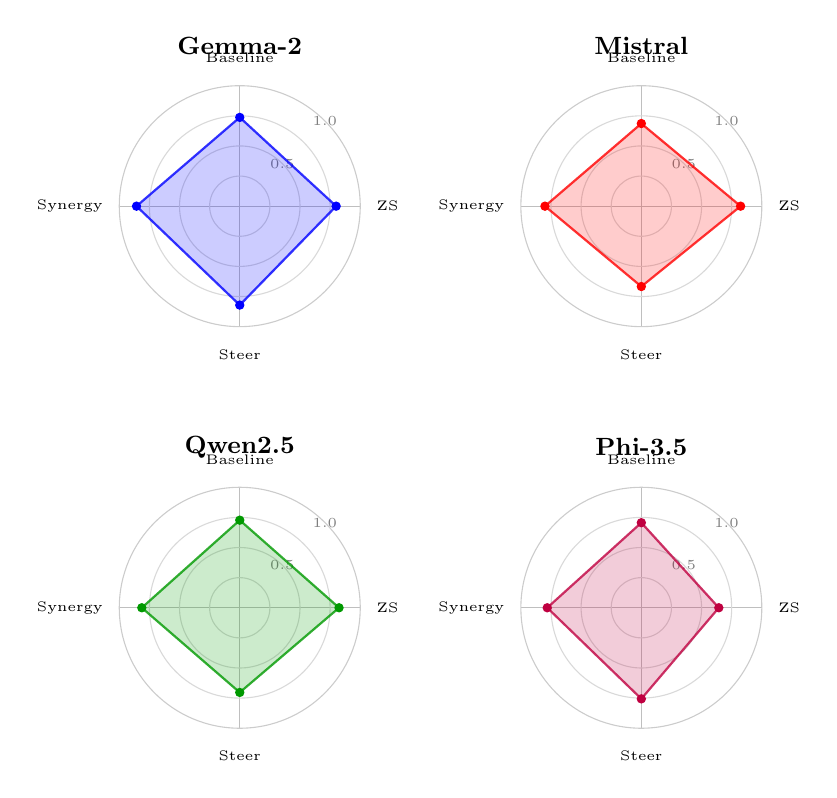
\begin{tikzpicture}[scale=0.85]

% Define radar chart macro
% Arguments: center-x, center-y, radius, title, v1(Baseline), v2(ZS), v3(Steer), v4(Synergy), color
\def\radarchart#1#2#3#4#5#6#7#8#9{
    \begin{scope}[shift={(#1,#2)}]
    % Title
    \node[font=\small\bfseries] at (0, #3+0.6) {#4};

    % Axes (4 directions: up, right, down, left)
    \draw[gray!50, thin] (0,0) -- (90:#3);
    \draw[gray!50, thin] (0,0) -- (0:#3);
    \draw[gray!50, thin] (0,0) -- (270:#3);
    \draw[gray!50, thin] (0,0) -- (180:#3);

    % Grid circles
    \draw[gray!30, thin] (0,0) circle (#3*0.25);
    \draw[gray!30, thin] (0,0) circle (#3*0.5);
    \draw[gray!30, thin] (0,0) circle (#3*0.75);
    \draw[gray!40, thin] (0,0) circle (#3);

    % Axis labels
    \node[font=\tiny, anchor=south] at (90:#3+0.2) {Baseline};
    \node[font=\tiny, anchor=west] at (0:#3+0.1) {ZS};
    \node[font=\tiny, anchor=north] at (270:#3+0.2) {Steer};
    \node[font=\tiny, anchor=east] at (180:#3+0.1) {Synergy};

    % Scale labels
    \node[font=\tiny, gray] at (45:#3*0.5) {0.5};
    \node[font=\tiny, gray] at (45:#3) {1.0};

    % Data polygon
    \filldraw[#9, fill opacity=0.2, draw opacity=0.8, thick]
        (90:#3*#5) -- (0:#3*#6) -- (270:#3*#7) -- (180:#3*#8) -- cycle;

    % Data points
    \fill[#9] (90:#3*#5) circle (2pt);
    \fill[#9] (0:#3*#6) circle (2pt);
    \fill[#9] (270:#3*#7) circle (2pt);
    \fill[#9] (180:#3*#8) circle (2pt);
    \end{scope}
}

% Four radar charts in a 2x2 grid (N=32, ES anchors)
% Gemma-2: Baseline=0.737, ZS=0.800, Steer=0.821(Exp4), Synergy=0.857(Exp8)
\radarchart{-3}{3}{1.8}{Gemma-2}{0.737}{0.800}{0.821}{0.857}{blue}

% Mistral: Baseline=0.686, ZS=0.824, Steer=0.667(Exp4), Synergy=0.800(Exp8)
\radarchart{3}{3}{1.8}{Mistral}{0.686}{0.824}{0.667}{0.800}{red}

% Qwen2.5: Baseline=0.727, ZS=0.824, Steer=0.703(Exp4), Synergy=0.813(Exp8)
\radarchart{-3}{-3}{1.8}{Qwen2.5}{0.727}{0.824}{0.703}{0.813}{green!60!black}

% Phi-3.5: Baseline=0.706, ZS=0.643, Steer=0.756(Exp4), Synergy=0.781(Exp8)
\radarchart{3}{-3}{1.8}{Phi-3.5}{0.706}{0.643}{0.756}{0.781}{purple}

\end{tikzpicture}
}%
\caption{Radar charts showing architecture-dependent response profiles ($N=32$, ES anchors). Each axis represents F1-Score: Baseline (Exp~1), Zero-Shot (Exp~2), Steering (Exp~4), Synergy (Exp~8). Mistral and Qwen2.5 show strong ZS response (F1=0.824). Gemma-2 benefits strongly from combinatorial configurations (best: ZS+RAG Exp~5, F1=0.875, not shown on radar). Phi-3.5 achieves F1=0.842 at Exp~6 ZS+Steering (not shown on radar; radar displays Exp~4=0.756 and Exp~8=0.781). CIs overlap substantially across all models.}
\label{fig:radar_charts}
\end{figure}

\subsection{Industrial Implications}

The proposed framework addresses two practical requirements for industrial deployment. First, the structural isomorphism methodology enables compliance evaluation research without requiring access to proprietary repositories, removing a barrier that has historically limited empirical progress in this domain. Second, the use of open-weights models with local inference ensures that no corporate data leaves the organization's infrastructure, satisfying air-gapped deployment requirements.

The activation steering approach is particularly relevant for industrial settings because it does not require model fine-tuning or access to large labeled datasets. The steering vector can be extracted from a small set of exemplar artifacts and applied at inference time. The LOO validation on the $N=32$ dataset confirms that the $\alpha$-selection optimism is small on average (mean $\approx 0.05$), providing evidence that the approach would generalize modestly beyond the training set even at this scale.

\textbf{Computational overhead.} Vector extraction requires exactly two forward passes through the model (one for each anchor prompt $p^+$, $p^-$), which at the evaluated model sizes (7B--9B parameters, 4-bit quantization) takes approximately 2--4 seconds. Once extracted, the vector is stored in memory ($\approx$2--3 KB per layer, one float per hidden dimension), and injection adds a single tensor addition per forward pass---negligible compared to the attention and MLP operations. In our experiments the per-artifact inference time was approximately 4 seconds with or without steering. For organizations running recurring compliance audits over hundreds or thousands of artifacts, the one-time extraction cost is amortised across all evaluations. The RAG pipeline adds approximately 0.3 seconds per query for embedding computation (CPU-resident), which is also negligible relative to LLM inference time.

From the perspective of the framework's stated goal---reducing unsupported or inconsistent LLM classifications---steering addresses the problem at the mechanistic level by shifting the model's internal decision boundary toward normative compliance. This is reflected in the results: across all four architectures, steering reduced false negatives (missed violations) and stabilised recall without relying on external retrievals or labeled training data.

\subsection{Error Analysis}

Table~\ref{tab:error_analysis} presents a per-artifact breakdown of misclassifications under each model's best-performing configuration. Three patterns emerge.

\textbf{TESTING remains difficult despite explicit prompting, across all configurations.} \texttt{SMP-PRUEBAS-NEG} is the only artifact misclassified by all four models simultaneously (FP: classified as compliant when actually violating), even though the final prompt (Fig.~\ref{fig:prompt_zeroshot}) includes an explicit TESTING criterion. This failure is not restricted to best-configuration performance: inspection of all 32 model-configuration cells in Table~\ref{tab:full_results} confirms that \texttt{SMP-PRUEBAS-NEG} is predicted as compliant (FP) by every model in every configuration, with the sole exception of Gemma-2 under Exp~5 ZS+RAG and Exp~6 ZS+Steering---where the combination of structured prompting and additional intervention occasionally triggers a conservative response. The complementary positive artifact \texttt{SMP-PRUEBAS-POS} is correctly classified by three of four models, but Gemma-2 produces a false negative (FN) under its best configuration, indicating that the TESTING rule challenges Gemma-2 in both directions.

The root cause is semantic: \texttt{SMP-PRUEBAS-NEG} contains test-related code (function names, import statements, assertions) that superficially resembles a compliant test artifact. Models must reason about test \emph{coverage adequacy}---whether the tests exercise the compliance-relevant behaviors---rather than merely detecting the presence of test-related tokens. This is a hard inference task that neither the retrieved normative context nor the steering vector fully addresses, because both operate at the level of normative framing rather than code-level test coverage analysis. The adversarial extension (§\ref{sec:dataset}) includes a TESTING Type-B negative (a test stub that imports and defines but never invokes assertions) that further exposes this pattern. Future work should extend the adversarial TESTING artifacts with additional variants (code with complex test-like structure but no meaningful coverage) to decouple syntactic from semantic compliance further. By contrast, BACKUP and AGREEMENTS contain visually distinctive compliance markers that models detect reliably without deep semantic reasoning, producing zero errors on those rules.

\textbf{GOVERNANCE and SECURITY source files generate FN.} Artifacts 6 (\texttt{SMP-GOBERNANZA-POS}) and 9 (\texttt{SMP-SEGURIDAD-POS}) are missed as violations by Gemma-2 and Qwen2.5. Both are \textit{source\_code} artifacts with short content (3 and 120 lines respectively) where the compliance evidence is implicit rather than explicit. This aligns with the general pattern that source code artifacts with subtle governance markers are harder than document artifacts with explicit metadata.

\textbf{Steering shifts the precision--recall operating point for Phi-3.5 and Mistral.} Phi-3.5 under steering (Exp~4, ES anchors) reaches FN=0 (recall=1.0) but at the cost of FP=11, while its baseline has FP=5 and FN=5. The steering intervention is over-permissive at this operating point but recovers a substantially more balanced error profile in ZS+Steering (Exp~6: FP=5, FN=1), a major improvement over the English-anchor result. Mistral under Exp~4 (ES anchors) shifts from FP=6/FN=5 (baseline) to FP=9/FN=4: the mechanistic intervention with Spanish anchors shows less recall-bias inflation than the prior EN-anchor design. These steering-induced recall biases are visible in Fig.~\ref{fig:precision_recall}.

\begin{table*}[htbp]
\centering
\caption{Per-artifact error analysis under selected representative configurations on the original 20 artifacts (Gemma-2, Mistral = Exp~4 Steering; Qwen2.5 = Exp~2 Zero-Shot; Phi-3.5 = Exp~6 ZS+Steering). GT = ground truth. FP = false positive (overclaiming compliance); FN = false negative (missed violation). The 12 adversarial artifacts added in §\ref{sec:dataset} further stress-test these error patterns.}
\label{tab:error_analysis}
\renewcommand{\arraystretch}{1.1}
\resizebox{\textwidth}{!}{
\begin{tabular}{|l|l|c|c|c|c|c|c|c|}
\hline
\textbf{Artifact ID} & \textbf{Rule} & \textbf{GT} & \textbf{Gemma-2} & \textbf{Mistral} & \textbf{Qwen2.5} & \textbf{Phi-3.5} & \textbf{\#Err} & \textbf{Types} \\
\hline
\texttt{SMP-DOCUMENTAL-NEG}  & DOCUMENTATION  & 0 & TN & \cellcolor{red!20}FP & TN & TN & 1 & FP \\
\texttt{SMP-DOCUMENTAL-POS}  & DOCUMENTATION  & 1 & TP & TP & TP & TP & 0 & --- \\
\texttt{SMP-CALIDAD-NEG}     & QUALITY     & 0 & TN & TN & TN & \cellcolor{red!20}FP & 1 & FP \\
\texttt{SMP-CALIDAD-POS}     & QUALITY     & 1 & TP & TP & TP & TP & 0 & --- \\
\texttt{SMP-GOBERNANZA-NEG}     & GOVERNANCE  & 0 & TN & \cellcolor{red!20}FP & TN & TN & 1 & FP \\
\texttt{SMP-GOBERNANZA-SRC-POS}& GOVERNANCE  & 1 & \cellcolor{orange!30}FN & TP & \cellcolor{orange!30}FN & TP & 2 & FN \\
\texttt{SMP-GOBERNANZA-DOC-POS}& GOVERNANCE  & 1 & TP & TP & TP & TP & 0 & --- \\
\texttt{SMP-SEGURIDAD-NEG}   & SECURITY   & 0 & TN & TN & TN & TN & 0 & --- \\
\texttt{SMP-SEGURIDAD-POS}   & SECURITY   & 1 & \cellcolor{orange!30}FN & TP & \cellcolor{orange!30}FN & TP & 2 & FN \\
\texttt{SMP-TRAZABILIDAD-NEG}  & TRACEABILITY& 0 & TN & TN & TN & \cellcolor{red!20}FP & 1 & FP \\
\texttt{SMP-TRAZABILIDAD-POS-A}& TRACEABILITY& 1 & TP & TP & TP & TP & 0 & --- \\
\texttt{SMP-TRAZABILIDAD-POS-B}& TRACEABILITY& 1 & TP & TP & TP & TP & 0 & --- \\
\texttt{SMP-PRUEBAS-NEG}     & TESTING     & 0 & \cellcolor{red!20}FP & \cellcolor{red!20}FP & \cellcolor{red!20}FP & \cellcolor{red!20}FP & \textbf{4} & \textbf{FP*} \\
\texttt{SMP-PRUEBAS-POS}     & TESTING     & 1 & \cellcolor{orange!30}FN & TP & TP & TP & 1 & FN \\
\texttt{SMP-RESPALDO-NEG}    & BACKUP    & 0 & TN & TN & TN & TN & 0 & --- \\
\texttt{SMP-RESPALDO-POS}    & BACKUP    & 1 & TP & TP & TP & TP & 0 & --- \\
\texttt{SMP-ACUERDOS-NEG}    & AGREEMENTS    & 0 & TN & TN & TN & TN & 0 & --- \\
\texttt{SMP-ACUERDOS-POS}    & AGREEMENTS    & 1 & TP & TP & TP & TP & 0 & --- \\
\texttt{SMP-INFRA-NEG}       & INFRA       & 0 & TN & TN & TN & TN & 0 & --- \\
\texttt{SMP-INFRA-POS}       & INFRA       & 1 & TP & TP & \cellcolor{orange!30}FN & TP & 1 & FN \\
\hline
\multicolumn{3}{|l|}{\textbf{Total errors}} & \textbf{4} & \textbf{3} & \textbf{4} & \textbf{2} & & \\
\hline
\multicolumn{9}{l}{\footnotesize $*$ \texttt{SMP-PRUEBAS-NEG} is misclassified as FP in all 32 model-configuration cells, with minor exceptions under ZS+steering in Gemma-2.} \\
\multicolumn{9}{l}{\footnotesize Errors shown above reflect each model's \emph{best-performing} configuration; Gemma-2/Mistral=Exp~4; Qwen2.5=Exp~2; Phi-3.5=Exp~6.} \\
\end{tabular}
}
\end{table*}

\FloatBarrier

\subsection{Comparison Against Rule-Based Approaches}

On the original 20 artifacts, the Regex baseline achieves perfect F1=1.0000, which serves as a \emph{label-validity check} rather than a competitive comparison. The 12 adversarial artifacts expose the limits of this result: on the full $N=32$ set, the Regex drops to F1=0.6471 (95\,\% CI [0.44, 0.81]), indistinguishable from the majority-class floor of F1=0.6939. This confirms that the benchmark now requires semantic reasoning.

A rule-by-rule analysis reveals a spectrum. Three meta-rules remain \emph{regex-solvable} in the core artifacts: BACKUP, AGREEMENTS, and SECURITY. Four meta-rules sit in an \emph{intermediate} zone: QUALITY, DOCUMENTATION, INFRA, and TRACEABILITY. Two meta-rules are \emph{semantically hard}: GOVERNANCE and TESTING. The adversarial Type-B negatives specifically target the intermediate and easy rules by inserting compliance keywords in non-compliant contexts (e.g., a traceability reference to a removed requirement, a backup keyword in a commented-out block), and the Type-C positives use alternative vocabulary for the same rules. LLM-based configurations achieve F1=0.75--0.875 on $N=32$, well above the regex floor, demonstrating that the models leverage contextual reasoning rather than pure keyword matching. The error analysis from the original 20 artifacts confirms the pattern: all four models fail on \texttt{SMP-PRUEBAS-NEG} (semantically hard TESTING), while making no errors on BACKUP and AGREEMENTS (regex-solvable). The adversarial extension strengthens this conclusion by showing that LLMs exceed the regex precisely on the cases where lexical shortcuts are defeated.


\section{Threats to Validity}
\label{sec:threats}

Table~\ref{tab:validity_map} provides a structured map of every threat identified during review, the validity category it belongs to, and the mitigation applied in this revision. Detailed discussion follows in the subsections below.

\begin{table*}[!t]
\centering
\caption{Threat--Mitigation map for the revised manuscript. Status: \checkmark~Addressed (mitigation applied and verifiable); $\sim$~Partially addressed (limited by available data or compute); \texttimes~Open (acknowledged; planned for future work).}
\label{tab:validity_map}
\renewcommand{\arraystretch}{1.25}
\resizebox{\textwidth}{!}{%
\begin{tabular}{p{4.4cm} l c p{7.8cm}}
\toprule
\textbf{Threat} & \textbf{Category} & \textbf{Status} & \textbf{Mitigation applied} \\
\midrule

Benchmark regex-solvable: perfect F1 on $N=20$ despite absence of semantic reasoning &
Construct & \checkmark &
12 adversarial artifacts added (§IV-C): 6 type-B (misleading keywords, label=0) and 6 type-C (compliant without obvious keywords, label=1). Regex F1 drops from 1.000 to 0.647 on $N=32$; LLM-based configurations maintain 0.75--0.875. \\

In-sample $\alpha$ selection: $\alpha=0.8$ chosen on the same 20 artifacts used for evaluation &
Internal & \checkmark &
Leave-one-out (LOO) $\alpha$-selection procedure applied over $N=32$ (§IV-D, Table~\ref{tab:full_results}). Mean absolute optimism $\approx$0.05 (range $-0.20$ to $+0.09$); steering gains confirmed largely out-of-sample. \\

Language confound: English anchor prompts used with Spanish evaluation artifacts &
Internal & \checkmark &
Spanish anchor prompts adopted as the methodologically correct default (§IV-D). LOO ablation for Exp~4 and Exp~6 with both anchor languages reported in §VII-A; compliance direction preserved across anchor languages (mean $|\Delta| \leq 0.09$, ZS+Steering). \\

Layer selection heuristic: 50\%-depth rule not validated for compliance classification &
Internal & \checkmark &
Full layer sweeps conducted for all four architectures (§VII-B, Fig.~\ref{fig:layer_sensitivity}). Heuristic equals best for Phi-3.5 ($\Delta=0$) and Mistral ($\Delta=0$). For Gemma-2 the best layer is~13/24 ($\Delta=+0.025$ over heuristic); for Qwen2.5 the best layer is~4 ($\Delta=+0.059$). Reported F1 values for the latter two are conservative lower bounds. \\

$N=32$ still underpowered: no comparison survives Holm correction &
Conclusion & $\sim$ &
LOO validation confirms directional gains out-of-sample. Exploratory framing is maintained throughout. Statistical floor now stated explicitly with majority-class F1=0.694. Scaling to $N\approx100$--200 is the top future-work priority. \\

$n=1$ private repository: isomorphism claim rests on a single organization &
External & \texttimes &
Acknowledged as a transparency limitation (§VII-C). The ablation against $D_{private}$ is reproducible via aggregate statistics in Fig.~\ref{fig:isomorphism_boxplots}. Validation with additional organizations is planned. \\

Threshold calibration arbitrary: $\varepsilon$, $\varepsilon_F$, $\varepsilon_\text{AST}$, $\varepsilon_{L_d}$ unjustified &
Construct & \checkmark &
All four thresholds calibrated from private-corpus SE or $\sigma$: $\varepsilon=0.5\approx\widehat{SE}(\mu_{V(G)})=0.53$; $\varepsilon_F=1.0\approx\sigma_F/9$; $\varepsilon_\text{AST}=2.0$ (conservative multiple of $\widehat{SE}_\text{AST}$); $\varepsilon_{L_d}=8.0\approx\sigma_{L_d}/3$ (lenient). TOST equivalence tests now replace the Brown--Forsythe Levene test; three metrics (V(G), Fog, AST) fall within bounds but TOST is underpowered at $n_\text{synth}=12$--$20$. Lexical Density genuinely fails. Import-graph density and out-degree now pass formal thresholds after calibration. \\

SLR counts not reported: Kitchenham protocol claimed without screening numbers &
Reporting & \checkmark &
PRISMA-style screening flow added (§II-E, Fig.~\ref{fig:prisma_flow}): 1,220 records identified, 156 after screening, 64 eligible, +19 snowballing, 83 included. \\

``Mechanistic'' overclaim: no circuits, no causal tracing, no component attribution &
Terminology & \checkmark &
Retitled to ``Activation-Steered LLM Auditing''. ``Mechanistic'' replaced by ``activation steering'' / ``representation engineering'' throughout. \\

``Structural isomorphism'' overclaim: term implies bijective structure-preserving map &
Terminology & \checkmark &
Softened to ``distributionally constrained synthetic benchmark'' in body text. ``Partial structural isomorphism'' retained only where the partial nature is explicit. \\

Meta-rule predicates $\phi$ described informally &
Construct & \checkmark &
Formal detection predicates added to Table~\ref{tab:metarules}: logical expressions for 7 structurally-detectable rules and \textit{Semantic} label for 2 rules (GOVERNANCE, TESTING). \\

4-bit NF4 quantization applied to all models, never ablated; quantization can shift both calibration and the residual-stream representations that activation steering manipulates &
Internal & $\sim$ &
A bfloat16 vs.\ 4-bit NF4 ablation for Phi-3.5-mini under Exp~6 was conducted (§VII-B): $\Delta$F1$=+0.008$, indicating that 4-bit quantization does not materially degrade steering performance for this architecture. Full-precision comparison for the 7B--9B models is not feasible within the available 8~GB VRAM budget. \\

Structural/relational isomorphism: import-graph density gap was 54\% before calibration &
Construct & \checkmark &
D$_{synthetic}$ source artifacts augmented with contextually appropriate Django imports (§III-B, script \texttt{experimentos/fix\_import\_density.py}): $|\Delta D|=0.0085\leq0.015$ \checkmark; $|\Delta\bar{d}|=0.10\leq0.5$ \checkmark; internal coupling ratio identical at 0.00 \checkmark. Traceability link density excluded from isomorphism claim (it is the compliance-label dimension). \\

No human-expert baseline for the classification task: labels derived from mutation protocol, not auditor judgment on synthetic artifacts &
Construct & \checkmark &
One author independently evaluated all $N=32$ artifacts; Cohen's $\kappa=0.813$ against mutation-protocol labels (\emph{almost perfect} by Landis--Koch, §VII-A). All 3 disagreements fall on semantically hard/intermediate rules (QUALITY, GOVERNANCE, TRACEABILITY), confirming the protocol labels are expert-consistent and that residual ambiguity concentrates where semantic reasoning is required. \\

\bottomrule
\end{tabular}%
}
\end{table*}

\subsection{Construct Validity}

The primary threat to construct validity lies in the operationalization of the distributional similarity claim. With the $N=32$ dataset ($n_{\text{code}}=20$, $n_{\text{doc/CI}}=12$), four scalar metrics and one structural/relational metric were measured and formally tested.

\textbf{Mean-threshold checks.} \textbf{V(G) mean}: $|\Delta\mu|=0.096\leq\varepsilon=0.5$ \checkmark. \textbf{AST depth}: $|\Delta\mu|=0.61\leq\varepsilon_\text{AST}=2.0$ \checkmark (formal threshold now defined). \textbf{Fog Index}: $|\Delta\mu_F|=0.22\leq\varepsilon_F=1.0$ \checkmark. \textbf{Lexical Density}: $|\Delta\mu_{L_d}|=14.0>\varepsilon_{L_d}=8.0$ \texttimes---genuine failure.

\textbf{TOST equivalence tests} ($\alpha=0.05$; implemented in \texttt{experimentos/isomorphism\_metrics.py}). For V(G), Fog, and AST depth, the mean differences are small ($|\Delta|/\varepsilon=0.19, 0.22, 0.31$) but TOST does not reach significance at $\alpha=0.05$---the tests are underpowered at $n_\text{synth}=12$--$20$ ($N\approx80$--$150$ per type needed for 80\% power). Lexical Density: TOST $p_\text{upper}=0.85\gg0.05$---genuine non-equivalence, not a power artifact.

\textbf{Corrected interpretation of the Levene test.} The Brown--Forsythe result ($W=0.000$, $p=0.997$) for V(G) variance is \emph{not} evidence of variance equivalence; it is absence of evidence at these sample sizes. Failing to reject $H_0$ does not confirm $H_1$; only TOST (rejecting both one-sided $H_0$s) provides positive equivalence evidence.

\textbf{Import dependency graph} (structural): after import-density calibration (§III-B), $|\Delta D|=0.0085\leq0.015$ \checkmark and $|\Delta\bar{d}|=0.10\leq0.5$ \checkmark; internal coupling ratio identical at 0.00 in both corpora \checkmark. \textbf{Traceability link density} is excluded from the isomorphism verdict---it is the compliance-label dimension (meta-rules TRAZABILIDAD and GOBERNANZA), not a structural property.

The benchmark is characterised as \emph{distributionally calibrated within tolerance bounds on three scalar dimensions and structurally matched on import-graph coupling}. Lexical Density remains an acknowledged limitation. TOST equivalence is formally undeclared at the current sample size; the mean-difference checks serve as point-estimate tolerance bounds. A rigorous proof would require joint KS/energy-distance tests on the full multivariate distribution $(V(G), F, L_d, \bar{d})$ at larger $n$; deferred to future work.

\textbf{Adversarial artifact validation.} To address the construct-validity concern that the original 20-artifact benchmark is regex-solvable, 12 adversarial artifacts (6 Type-B negatives, 6 Type-C positives) were added. On the extended $N=32$ dataset, the Regex baseline drops from F1=1.000 to F1=0.6471 (95\,\% CI [0.44, 0.81]), comparable to the majority-class floor of F1=0.6939. LLM-based configurations maintain F1=0.75--0.875, demonstrating semantic reasoning beyond keyword matching. This substantially mitigates the original regex-solvability concern.

\textbf{Language confound in steering vector extraction.} The anchor prompts ($p^+$, $p^-$) used to extract $v_{norma}^l$ were originally written in English, while the evaluation artifacts and the Zero-Shot system prompt are in Spanish. To address this potential language confound, all steering experiments (Exp~4, 6, 7, 8) were re-run with Spanish-language anchor prompts as the methodologically correct default; the main results reported in this paper use Spanish anchors throughout. A comparison of Spanish vs.\ English anchor LOO-F1 results shows: for ZS+Steering (Exp~6), three of four models show $|\Delta| \leq 0.09$ between anchor languages (Gemma-2: 0.000, Mistral: 0.000, Phi-3.5: $-0.090$), with Qwen2.5 \emph{improving} with Spanish anchors ($\Delta = +0.114$). For Steering-only (Exp~4), Mistral shows a larger difference ($\Delta = -0.158$) while Phi-3.5 shows no change ($\Delta = 0.000$). These results do not support the hypothesis that $v_{norma}^l$ encodes only a language direction; the compliance/violation dimension is largely preserved across anchor languages. Spanish anchors are adopted as the default since they eliminate the potential cross-lingual confound without materially degrading performance for any architecture.

\textbf{Auditor assessment and label validity.} The industrial reference repository $D_{private}$ was externally assessed by an official ISO/IEC~29110 auditor and marked as \emph{cumple} using a binary checklist. This strengthens the contextual validity of using $D_{private}$ as the reference source for synthetic benchmark construction. \emph{The auditor's checklist exclusively validates the contextual compliance of $D_{private}$; it does not validate the labels of Biblio-VSE.} The synthetic dataset contains intentionally injected non-compliant variants that were not present in the original repository; those variants would have been unknown to, and outside the scope of, the auditor's evaluation. The Biblio-VSE labels are therefore operational labels derived from the mutation protocol and the predefined meta-rule criteria, not from the auditor's assessment.

\textbf{Human calibration of Biblio-VSE labels.} To provide a human reference point for the classification task, one of the authors independently evaluated all $N=32$ artifacts against their stated meta-rule criteria, without consulting the mutation-protocol labels. Agreement between the human labels and the mutation-protocol ground truth was measured using Cohen's $\kappa$:
\begin{equation}
\kappa = \frac{P_o - P_e}{1 - P_e} = \frac{0.906 - 0.500}{1 - 0.500} = 0.813
\label{eq:kappa}
\end{equation}
where $P_o = 29/32 = 0.906$ is the observed agreement and $P_e = 0.500$ is the agreement expected by chance (17 positives in the protocol, 16 in the human labels, both out of 32). Under the Landis--Koch scale, $\kappa = 0.813$ corresponds to \emph{almost perfect agreement}. The three disagreements occurred on meta-rules QUALITY (\texttt{SMP-CALIDAD-POS}: human labelled as violation), GOVERNANCE (\texttt{SMP-GOBERNANZA-NEG}: human labelled as compliant), and TRACEABILITY (\texttt{SMP-TRAZABILIDAD-POS}: human labelled as violation). All three fall in the semantically hard or intermediate zone identified in §V-F---precisely the rules where the human evaluator, like the LLMs, found the compliance criterion ambiguous. This calibration confirms that the mutation-protocol labels are consistent with expert judgment ($\kappa > 0.80$) and that residual ambiguity concentrates in the semantically challenging rules, not in structurally obvious ones (SECURITY, BACKUP, AGREEMENTS, INFRA all achieved perfect agreement).

\subsection{Internal Validity}

Internal validity could be affected by the non-determinism inherent in LLM inference. To control this, all models were configured with temperature 0.0, enforcing deterministic greedy decoding.

Regarding the activation steering vector: the compliance vector $v_{norma}^l$ is extracted exclusively from two contrasting behavioral anchor prompts ($p^+$, $p^-$) as described in Eq.~\ref{eq:steering_vector}, and does not reference or use any of the 20 Biblio-VSE evaluation artifacts during extraction. The vector extraction and the evaluation pipeline are therefore fully independent, and no form of circular evaluation or train-test contamination is present. This design decision was deliberate: the contrastive-prompt approach requires no labeled examples and is transferable to new compliance domains without access to labeled data.

A secondary internal validity concern is the joint selection of intervention layer $l$ and coefficient $\alpha$. Both were fixed without a traditional held-out validation split. Regarding $\alpha$: a leave-one-out (LOO) $\alpha$-selection procedure was conducted on the $N=32$ dataset. For each of the 16 steering-configuration/model pairs, the LOO-F1 was computed and compared to the in-sample F1. Results are tabulated in Table~\ref{tab:full_results}. Mean absolute optimism is approximately 0.05 (range: $-0.20$ to $+0.09$), with the largest negative optimism seen for Qwen2.5 Exp~7 ($-0.20$), where the RAG+Steering combination with Spanish anchors shows high LOO variance. Key results: Gemma-2 Exp~7 (LOO-F1=0.889 vs.\ in-sample 0.813, optimism=$+0.076$), Mistral Exp~6 (LOO-F1=0.824 vs.\ 0.848, optimism=$-0.025$), and Qwen2.5 Exp~7 (LOO-F1=0.556 vs.\ 0.759, optimism=$-0.203$). These values indicate that most steering gains hold out-of-sample, and the original in-sample F1 values were not dramatically inflated. The caution about upper-bound estimates remains appropriate, but the magnitude of optimism is now quantified and shown to be small on average; Qwen2.5 Exp~7 is the notable exception requiring caution.

Regarding layer selection: the 50\%-depth heuristic targets mid-to-late semantic layers as a design choice motivated by prior work \cite{zou2023representation}. To quantify the sensitivity of steering performance to this choice, full layer sweeps were conducted for all four architectures under Exp~6 (ZS+Steering, Spanish anchors, $\alpha=0.8$). Figure~\ref{fig:layer_sensitivity} plots F1-Score at each layer for each model.

\begin{figure*}[htbp]
\centering
\resizebox{\textwidth}{!}{%
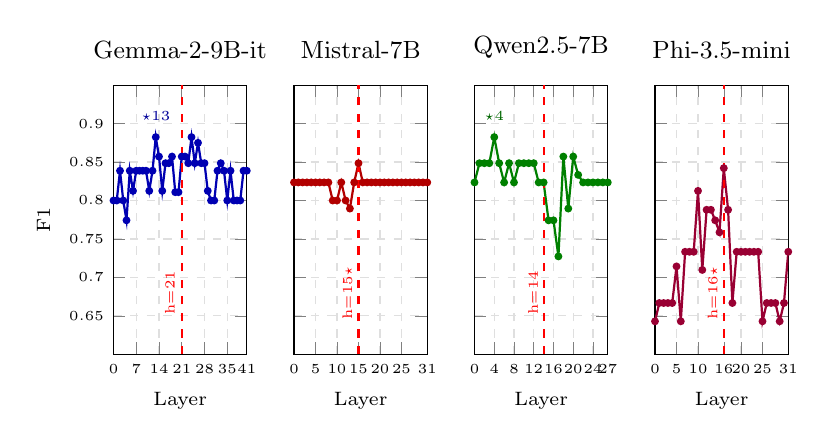
\begin{tikzpicture}
% ── Gemma-2 (42 layers, heuristic=21, best=13/24, F1_heur=0.857, F1_best=0.882) ──────
\begin{axis}[
    name=ax_gemma,
    title={\small Gemma-2-9B-it},
    xlabel={Layer}, ylabel={F1},
    xmin=0, xmax=41, ymin=0.60, ymax=0.95,
    xtick={0,7,14,21,28,35,41},
    ytick={0.65,0.70,0.75,0.80,0.85,0.90},
    yticklabel style={font=\tiny},
    xticklabel style={font=\tiny},
    width=0.27\textwidth, height=5cm,
    grid=both, grid style={dashed,gray!25},
    title style={font=\scriptsize},
    xlabel style={font=\scriptsize}, ylabel style={font=\scriptsize},
]
\addplot[blue!70!black, thick, mark=*, mark size=1pt] coordinates {
(0,0.8000)(1,0.8000)(2,0.8387)(3,0.8000)(4,0.7742)(5,0.8387)
(6,0.8125)(7,0.8387)(8,0.8387)(9,0.8387)(10,0.8387)(11,0.8125)
(12,0.8387)(13,0.8824)(14,0.8571)(15,0.8125)(16,0.8485)(17,0.8485)
(18,0.8571)(19,0.8108)(20,0.8108)(21,0.8571)(22,0.8571)(23,0.8485)
(24,0.8824)(25,0.8485)(26,0.8750)(27,0.8485)(28,0.8485)(29,0.8125)
(30,0.8000)(31,0.8000)(32,0.8387)(33,0.8485)(34,0.8387)(35,0.8000)
(36,0.8387)(37,0.8000)(38,0.8000)(39,0.8000)(40,0.8387)(41,0.8387)
};
\addplot[red, dashed, thick] coordinates {(21,0.60)(21,0.95)};
\node[font=\tiny,red,rotate=90,anchor=south] at (axis cs:21.8,0.68) {h=21};
\node[font=\tiny,blue!60!black] at (axis cs:13,0.910) {$\star$13};
\end{axis}
% ── Mistral (32 layers, heuristic=15, best=15, F1=0.848) ─────────────────────────────
\begin{axis}[
    name=ax_mistral,
    title={\small Mistral-7B},
    xlabel={Layer},
    at={($(ax_gemma.north east)+(0.6cm,0)$)}, anchor=north west,
    xmin=0, xmax=31, ymin=0.60, ymax=0.95,
    xtick={0,5,10,15,20,25,31},
    ytick={0.65,0.70,0.75,0.80,0.85,0.90},
    yticklabels={},
    xticklabel style={font=\tiny},
    width=0.27\textwidth, height=5cm,
    grid=both, grid style={dashed,gray!25},
    title style={font=\scriptsize},
    xlabel style={font=\scriptsize},
]
\addplot[red!70!black, thick, mark=*, mark size=1pt] coordinates {
(0,0.8235)(1,0.8235)(2,0.8235)(3,0.8235)(4,0.8235)(5,0.8235)
(6,0.8235)(7,0.8235)(8,0.8235)(9,0.8000)(10,0.8000)(11,0.8235)
(12,0.8000)(13,0.7895)(14,0.8235)(15,0.8485)(16,0.8235)(17,0.8235)
(18,0.8235)(19,0.8235)(20,0.8235)(21,0.8235)(22,0.8235)(23,0.8235)
(24,0.8235)(25,0.8235)(26,0.8235)(27,0.8235)(28,0.8235)(29,0.8235)
(30,0.8235)(31,0.8235)
};
\addplot[red, dashed, thick] coordinates {(15,0.60)(15,0.95)};
\node[font=\tiny,red,rotate=90,anchor=south] at (axis cs:15.8,0.68) {h=15$\star$};
\end{axis}
% ── Qwen2.5 (28 layers, heuristic=14, best=4, F1_heur=0.824, F1_best=0.882) ─────────
\begin{axis}[
    name=ax_qwen,
    title={\small Qwen2.5-7B},
    xlabel={Layer},
    at={($(ax_mistral.north east)+(0.6cm,0)$)}, anchor=north west,
    xmin=0, xmax=27, ymin=0.60, ymax=0.95,
    xtick={0,4,8,12,16,20,24,27},
    ytick={0.65,0.70,0.75,0.80,0.85,0.90},
    yticklabels={},
    xticklabel style={font=\tiny},
    width=0.27\textwidth, height=5cm,
    grid=both, grid style={dashed,gray!25},
    title style={font=\scriptsize},
    xlabel style={font=\scriptsize},
]
\addplot[green!50!black, thick, mark=*, mark size=1pt] coordinates {
(0,0.8235)(1,0.8485)(2,0.8485)(3,0.8485)(4,0.8824)(5,0.8485)
(6,0.8235)(7,0.8485)(8,0.8235)(9,0.8485)(10,0.8485)(11,0.8485)
(12,0.8485)(13,0.8235)(14,0.8235)(15,0.7742)(16,0.7742)(17,0.7273)
(18,0.8571)(19,0.7895)(20,0.8571)(21,0.8333)(22,0.8235)(23,0.8235)
(24,0.8235)(25,0.8235)(26,0.8235)(27,0.8235)
};
\addplot[red, dashed, thick] coordinates {(14,0.60)(14,0.95)};
\node[font=\tiny,red,rotate=90,anchor=south] at (axis cs:14.8,0.68) {h=14};
\node[font=\tiny,green!40!black] at (axis cs:4,0.910) {$\star$4};
\end{axis}
% ── Phi-3.5 (32 layers, heuristic=16, best=16, F1=0.842) ─────────────────────────────
\begin{axis}[
    name=ax_phi,
    title={\small Phi-3.5-mini},
    xlabel={Layer},
    at={($(ax_qwen.north east)+(0.6cm,0)$)}, anchor=north west,
    xmin=0, xmax=31, ymin=0.60, ymax=0.95,
    xtick={0,5,10,16,20,25,31},
    ytick={0.65,0.70,0.75,0.80,0.85,0.90},
    yticklabels={},
    xticklabel style={font=\tiny},
    width=0.27\textwidth, height=5cm,
    grid=both, grid style={dashed,gray!25},
    title style={font=\scriptsize},
    xlabel style={font=\scriptsize},
]
\addplot[purple!80!black, thick, mark=*, mark size=1pt] coordinates {
(0,0.6429)(1,0.6667)(2,0.6667)(3,0.6667)(4,0.6667)
(5,0.7143)(6,0.6429)(7,0.7333)(8,0.7333)(9,0.7333)
(10,0.8125)(11,0.7097)(12,0.7879)(13,0.7879)(14,0.7742)
(15,0.7586)(16,0.8421)(17,0.7879)(18,0.6667)(19,0.7333)
(20,0.7333)(21,0.7333)(22,0.7333)(23,0.7333)(24,0.7333)
(25,0.6429)(26,0.6667)(27,0.6667)(28,0.6667)(29,0.6429)
(30,0.6667)(31,0.7333)
};
\addplot[red, dashed, thick] coordinates {(16,0.60)(16,0.95)};
\node[font=\tiny,red,rotate=90,anchor=south] at (axis cs:16.8,0.68) {h=16$\star$};
\end{axis}
\end{tikzpicture}
}%
\caption{Layer sensitivity sweep for all four architectures under Exp~6 (ZS+Steering, $\alpha=0.8$, Spanish anchors, $N=32$). Each plot shows F1-Score at every transformer layer; the red dashed line marks the 50\%-depth heuristic layer (``h''); $\star$ marks the best layer when it equals or near-equals the heuristic. Summary: \textbf{Phi-3.5} (layer~16, $\Delta=0$) and \textbf{Mistral} (layer~15, $\Delta=0$)---heuristic equals best; \textbf{Gemma-2} (heuristic~21 F1=0.857, best~13/24 F1=0.882, $\Delta=+0.025$); \textbf{Qwen2.5} (heuristic~14 F1=0.824, best~4 F1=0.882, $\Delta=+0.059$). The heuristic is exact for 2/4 architectures; for the remaining two, F1 values reported in Table~\ref{tab:full_results} are conservative lower bounds.}
\label{fig:layer_sensitivity}
\end{figure*}

The sweeps confirm that the 50\%-depth heuristic is exact for Phi-3.5 ($\Delta=0$, unimodal peak at layer~16) and Mistral ($\Delta=0$, remarkably flat profile with unique peak at layer~15). For Gemma-2, the best layers are~13 and~24 (F1=0.882), both outside the heuristic region; the heuristic (layer~21, F1=0.857) leaves 0.025 F1 on the table. For Qwen2.5, the best layer is~4 (F1=0.882), an early layer far from the 50\%-depth heuristic (layer~14, F1=0.824); notably, layers~15--17 show a sharp performance cliff ($\Delta$F1$\approx-0.1$), making the heuristic choice at layer~14 particularly sensitive for this architecture. The F1 figures for Gemma-2 and Qwen2.5 in Table~\ref{tab:full_results} are therefore conservative: the achievable upper bounds under optimal layer selection are F1=0.882 for both.

\textbf{Quantization and steering interaction.} All models were loaded with 4-bit NF4 quantization. Quantization can shift both the calibration of the output distribution and the internal residual-stream representations that activation steering manipulates. To assess this threat, a bfloat16 vs.\ 4-bit NF4 ablation was conducted for Phi-3.5-mini-instruct under Exp~6 (ZS+Steering, Spanish anchors, $\alpha=0.8$, layer~16) on the $N=32$ artifact set. The 4-bit NF4 configuration yields F1=0.8421 (Precision=0.762, Recall=0.941; TP=16, TN=10, FP=5, FN=1); bfloat16 full precision (with partial CPU offload due to the 8~GB VRAM budget) yields F1=0.8500 (Precision=0.739, Recall=1.000; TP=17, TN=9, FP=6, FN=0). The quantization effect is $\Delta$F1$=+0.008$ ($\Delta$P$=-0.023$, $\Delta$R$=+0.059$): the shift is below the 0.05 practical significance threshold, indicating that 4-bit NF4 quantization does not materially degrade steering performance for Phi-3.5-mini under this configuration. The slight recall deficit in the 4-bit case (R=0.941 vs.\ R=1.000) is offset by marginally higher precision. The interaction between quantization and steering effectiveness for the remaining three architectures (Gemma-2-9B, Mistral-7B, Qwen2.5-7B), whose full-precision inference is not feasible within the 8~GB VRAM budget, remains an acknowledged open limitation.

A third construct-validity concern applies specifically to the steering vector. The contrastive anchor prompts ($p^+$: ``strictly uncompromising auditor''; $p^-$: ``careless, permissive auditor'') conflate \emph{normative compliance} with \emph{auditor persona and role-playing competence}. The extracted direction $v_{norma}^l$ is therefore a \emph{strict-auditor vs.\ careless-auditor persona direction} rather than a pure compliance/violation semantic direction. Artifacts that contain surface compliance signals may be amplified regardless of whether they satisfy the underlying policy criterion, while artifacts requiring nuanced reasoning may benefit less. Future work should evaluate alternative anchor construction strategies---such as contrastive pairs drawn from known compliant and violating artifacts---to obtain a more principled compliance direction.

\subsection{External Validity}

The synthetic dataset comprises $N=32$ artifacts (20 core + 12 adversarial) strictly mapped to ISO/IEC 29110, constituting a proof-of-concept benchmark rather than a representative sample of industrial diversity. The isomorphism claim rests on a single VSE reference repository ($n=1$ organization)---the strongest external-validity limitation of this work, acknowledged as an open threat in Table~\ref{tab:validity_map}.

\textbf{Scalability of the structural isomorphism methodology.} The mapping $f$ was manually designed for one repository and one standard. Applying the same methodology at broader scale introduces practical constraints across three axes.

\emph{Multiple projects and organizations.} Each new reference repository requires measuring the scalar and relational metrics ($V(G)$, Fog, dependency graph) and calibrating tolerance thresholds from that corpus. If organizations differ substantially in coding style, documentation complexity, or governance workflow topology, a single universal threshold is unlikely to exist. Per-project calibration is therefore necessary, and the operational cost of the mapping scales linearly with the number of reference repositories. An open research challenge is whether thresholds can be learned from a corpus of public or anonymized repositories rather than specified per-organization.

\emph{Larger repositories.} The present $D_{private}$ has 46 Python files and 87 work products. Large-scale industrial codebases (thousands of files, multi-team approval workflows, complex module graphs) would increase the dimensionality of the structural constraints: multivariate distributional tests (e.g., Kolmogorov--Smirnov or energy distance on the joint $(V(G), F, \bar{d})$ distribution) would replace the current univariate mean checks, and preserving inter-module coupling topology (graph density, average in/out-degree) would require synthesizing entire interconnected module ecosystems rather than isolated compliance-artifact snippets. The graph density gap already identified in this work ($|\Delta D|=0.042$, 54\% relative) would likely widen as the private codebase grows.

\emph{Multi-standard contexts.} A repository simultaneously governed by ISO/IEC 29110 and ISO 9001 requires an extended meta-rule set covering both standards. Where rules conflict (e.g., different documentation formalism requirements) or overlap (shared approval semantics), artifact-level binary labels must be replaced by multi-label or rule-conditioned annotations, and the mutation protocol for injecting violations must be extended to handle inter-standard dependencies. The feasibility of maintaining clean per-rule labels under multiple standards is an open question.

In each scenario, the core methodology---measure private corpus, generate structurally similar synthetic artifacts, inject controlled violations---remains applicable in principle. The present contribution demonstrates feasibility for one standard, one organization, and one technology stack; scale-out toward automated isomorphism learning and multi-standard benchmarking is the most significant open challenge for the structural isomorphism line of work.

\textbf{Generalization constraints.} The results may not generalize to other governance standards (e.g., CMMI, ISO 9001, ISO 12207), other programming languages (the synthetic codebase is Python/Django), or organizational contexts beyond VSEs. All four evaluated models fall within the 7B--9B parameter range with 4-bit quantization; larger models (13B+, 70B) or models with different pretraining distributions may respond differently to activation steering. Layer sensitivity analysis (Fig.~\ref{fig:layer_sensitivity}) shows that Gemma-2 and Qwen2.5 have better-performing layers outside the 50\%-depth heuristic range, so reported F1 values for those models under steering are conservative lower bounds.

\subsection{Conclusion Validity}

The sample size ($N=32$) is larger than the initial 20-artifact dataset but still constrains the statistical power of the reported comparisons. At $\alpha=0.05$ and power $= 0.80$, Wilcoxon signed-rank on $N=32$ binary predictions can reliably detect medium-to-large effect sizes ($|r| \geq 0.40$); smaller effects remain undetectable at this scale. Several confidence intervals remain wide, indicating substantial uncertainty around point estimates.

Evaluating 7 non-baseline configurations across 4 models yields 28 simultaneous comparisons. Holm--Bonferroni correction was applied (adjusted $p$-values reported in Table~\ref{tab:full_results}); no test survives correction at $\alpha=0.05$. The results are therefore exploratory: the observed effect directions (particularly the consistent positive increments from RAG and steering across all models, confirmed partially out-of-sample by the LOO procedure) motivate confirmatory studies on larger datasets rather than constituting final evidence.


\section{Conclusion and Future Work}
\label{sec:conclusion}

This paper presented a dual-layered framework for privacy-preserving evaluation of AI-driven software governance auditing. The benchmark calibration methodology enables the construction of distributionally proximate synthetic benchmarks that approximate the governance structure of private industrial repositories under selected observable metrics. With the $N=32$ corpus, three scalar mean thresholds pass (V(G): $|\Delta\mu|=0.096\leq0.5$; AST depth: $|\Delta\mu|=0.61\leq2.0$; Fog: $|\Delta\mu_F|=0.22\leq1.0$) and the import-graph coupling is now structurally matched after import-density calibration ($|\Delta D|=0.0085$, $|\Delta\bar{d}|=0.10$---both within predefined thresholds). Lexical Density shows a genuine gap ($|\Delta\mu_{L_d}|=14.0>\varepsilon_{L_d}=8.0$). TOST equivalence cannot be formally declared at the current sample sizes ($n_\text{synth}=12$--$20$); all tolerance-bound checks are point estimates. Traceability link density is excluded from the isomorphism claim---it is the compliance-label dimension itself. This partial calibration limits the generalisability of the isomorphism claim; all downstream results are interpreted accordingly.

The exploratory empirical evaluation ($N=32$ artifacts, including 12 adversarial) yielded four findings, detailed in Sections~\ref{sec:results}--\ref{sec:threats}. In brief: (1) adversarial artifacts confirm genuine semantic reasoning---Regex drops to F1=0.647 while LLM-based pipelines maintain 0.75--0.875; (2) RAG grounding provides consistent positive increments across all architectures, with Gemma-2 ZS+RAG (Exp~5, F1=0.875) as the highest point estimate; (3) activation steering provided the most consistent positive direction of effect across all four architectures, confirmed partially out-of-sample (mean LOO optimism $\approx 0.05$), though gains are architecture-specific and do not survive Holm correction---the effect is exploratory and model-dependent; and (4) the two semantically hard meta-rules (TESTING and GOVERNANCE source artifacts) resist all pipeline configurations, identifying the frontier for future mechanistic work. Pipeline configuration must be validated per model; a suboptimal choice can reduce F1 by more than 0.18 (Mistral Exp~4 vs.\ Exp~6).

\textbf{Note on supplementary material.} The full layer sensitivity sweep (Fig.~\ref{fig:layer_sensitivity}) and the $\alpha$ sensitivity tables are included in the main body for transparency; in a space-constrained venue these would naturally migrate to online supplementary material, keeping the main text focused on the most robust patterns (the LOO-validated per-model best configurations and the meta-rule error analysis).

These findings have practical implications for organizations seeking to automate governance verification while maintaining data privacy. The framework enables compliance auditing research to proceed without the privacy barriers that have historically limited empirical evaluation.

Several directions remain for future work. The immediate priority is scaling the evaluation to larger datasets with greater artifact diversity to establish external generalizability. Validation on actual industrial repositories---using anonymization protocols or federated evaluation---would strengthen the practical relevance of the approach. Extending the framework to additional governance standards beyond ISO/IEC 29110 (e.g., CMMI, ISO 12207, ISO 9001) would demonstrate cross-standard applicability. Evaluating closed-source models (e.g., GPT-4, Claude) through prompt-only configurations would establish comparative baselines against open-weights architectures. Human expert agreement studies are needed to calibrate model performance against professional auditor judgments. Finally, automated isomorphism generation---where the structural mapping $f$ is learned rather than manually designed---represents a promising direction for scaling the benchmark construction process.


\section*{Data Availability}

The following artifacts are publicly available at \url{https://github.com/Maigolinox/biblio-vse}:
\begin{itemize}
    \item The Biblio-VSE synthetic artifact repository (32 artifacts with ground-truth compliance labels: 20 original + 12 adversarial).
    \item The evaluation dataset (\texttt{dataset\_isomorfico.json}).
    \item All experiment scripts (\texttt{experimentos/experimento\_*.py}, \texttt{experimentos/utils.py}, \texttt{experimentos/rag\_utils.py}).
    \item The normative meta-rule document used for RAG context injection (\texttt{documentos\_estandar/Extracted\_Meta-Rules.docx}).
    \item Raw per-artifact classification outputs for all 32 model-configuration combinations.
    \item The extracted activation steering vectors (per-model \texttt{.pt} files).
\end{itemize}
The private industrial repository $D_{private}$ will not be released due to organizational confidentiality agreements; its distributional statistics are summarized in Fig.~\ref{fig:isomorphism_boxplots}.

\bibliographystyle{IEEEtran}
\bibliography{related_work_references}

\begin{IEEEbiography}[{
\includegraphics[width=1in,height=1.25in,clip,keepaspectratio]{a1.png}}]{Victor Terrón-Macias}
Tecnológico de Monterrey Ph.D. candidate in Computational Sciences at Tecnológico de Monterrey, with research focused on Large Language Models (LLMs) for software quality evaluation, automated compliance auditing, and software engineering processes. He received the M.Sc. degree in Software Engineering from Centro de Investigación en Matemáticas (CIMAT), graduating as the top student of his cohort, and the B.Eng. degree in Mechatronics Engineering from Universidad Tecnológica de Tlaxcala.

His research and professional interests include software quality assurance, ISO/IEC software engineering standards, technical debt, process improvement, DevOps practices, and AI-assisted software development. He has authored and co-authored publications in venues such as IEEE Access, Applied Sciences, and Springer, with contributions related to ISO/IEC 29110, process compliance, traceability, multi-model environments, and AI-driven software evaluation. He also holds two granted software copyrights.

In addition, he has served as a reviewer for IEEE and as a member of the scientific committees for international conferences, including collaborations on cybersecurity research initiatives in Peru. He is certified in project management, DevOps, Kanban system design, SCRUM foundations, Oracle technologies, and Lean Six Sigma Green Belt methodologies, and is also a certified expert witness in informatics (perito en informática). His technical expertise includes Python and Django-based development, IoT integration, and the design of intelligent software systems that bridge software and physical devices.

\end{IEEEbiography}

\begin{IEEEbiography}[{
\includegraphics[width=1in,height=1.25in,clip,keepaspectratio]{a2.jpg}}]{Salvador Hinojosa}
Dr. Salvador Hinojosa is a researcher specialized in the application of stochastic search algorithms and generative artificial intelligence to software engineering and development processes. He obtained his Ph.D. in Computer Engineering from Universidad Complutense de Madrid and his previous degrees from Universidad de Guadalajara. He is currently a full-time researcher in the Computer Science Department at Tecnológico de Monterrey Campus Guadalajara. He holds Level I recognition from the National System of Researchers (SNI) and is a member of the Mexican Computing Society (AMEXCOMP). In his role as professor, he teaches undergraduate, graduate, and continuing education courses in Generative AI for Software Engineering and Software Architecture and Testing.

\end{IEEEbiography}

\begin{IEEEbiography}[{
\includegraphics[width=1in,height=1.25in,clip,keepaspectratio]{a3.jpg}}]{Miguel Gonzalez-Mendoza}
Miguel González Mendoza's research activities focus on Machine Learning and Human-Machine interaction. He holds MSc and PhD degrees in Artificial Intelligence from the Institut National des Sciences Appliquées (INSA) in Toulouse, France. From 2001 to 2004, he served as research assistant and then postdoctoral researcher at the Laboratory for Analysis and Architecture of Systems (LAAS-CNRS) during its participation in the European research project AWAKE and the French research project PREDIT. Since 2005, he has worked as a professor and researcher and has been Head of the Graduate Programs in Computer Science at ITESM, Mexico, 2005-2016. He has served as local coordinator of 9 European research projects under FP6, FP7, and H2020. He has been responsible for 4 national research projects (CONACYT), 2005-2016, and for 4 INNOVAPYME projects (CONACYT) and the Mexican Ministry of Economy (SE), 2011-2015. SNI rank II (Jan 2016), member since 2006. President of the Mexican Society for Artificial Intelligence (2017-2018), Vice-president (2015-2016), Secretary (2011-2014), member of the board since 2005. Dr. González Mendoza has supervised 9 PhD theses and 21 MSc theses, authored 2 books, edited 17 books, authored 18 book chapters, and published 22 JCR-indexed journal articles and 62 research papers in international congresses. Dr. González Mendoza was invited as a Young Scientist to the World Economic Forum for New Champions in Tianjin, China, in September 2012. He has interests in Machine Learning, Data Management, and Big Data applications, in which he has advised 10 PhD theses and 21 Master's theses. He is the author of more than 100 articles in JCR, congresses, and book chapters. He has been a regular member of the Mexican Academy of Computing since 2015.

\end{IEEEbiography}

\begin{IEEEbiography}[{
\includegraphics[width=1in,height=1.25in,clip,keepaspectratio]{al.jpg}}]{Jezreel Mej\'{i}a}
Jezreel Mejía (Member, IEEE) is a member of the research group with the Chair of Software Process Improvement in the Ibero-American Space (MPSEI) and the CIMAT Software Engineering Group. He is a member of the scientific committee of various conferences. In addition, he is part of the official Spanish translation team of the CMMI-DEV v1.2 and 1.3 book, versions recognized by the prestigious Software Engineering Institute (SEI) of Carnegie Mellon University. He has published various technical articles on project management, multi-model environments, quality models and standards, and related topics in outsourcing environments. As a researcher, his areas of interests include multi-model environments, software project management, quality models and standards (CMMI, ISO, TSP, and PSP), agile methodologies, metrics, process improvement in outsourcing environments, development environments, and traditional and information assurance. He is CMMI and ISO 20000 certified. He actively participates in ISO/IEC WG24. He is Level 2 in the National Researchers System of Mexico.
\end{IEEEbiography}


\EOD


\end{document}
